%!TEX root = ../../../adrien_gomar_phd.tex
\chapter{Isolated low-speed CROR configuration}
\label{cha:dream_ls_isolated}

\chabstract{The studies performed in the previous chapters 
are finally used together to simulate the aeroelasticity
of a low-speed CROR configuration. First,
the steady results are analyzed to provide insight into the flow
physics and give confidence in the results. The prediction tool
defined in Chap.~\ref{cha:limitations_convergence}
is then used to estimate the number of harmonics required to
simulate the unsteady rigid-motion response 
of the CROR using the harmonic balance approach.
Aeroelastic simulations are then carried-out using the 
\replaced{decoupled}{weak-coupling}
approach that has been validated in the previous chapter. The OPT
algorithm develop in Chap.~\ref{cha:limitations_condition_number}
is used to ensure the stability of the computations.
Local excitation contours and the integrated damping are finally
analyzed.}


\newpage

\section{Presentation of the case}
\label{sec:dream_presentation}
%!TEX root = ../../../adrien_gomar_phd.tex


\begin{figure}[htp]
  \centering
  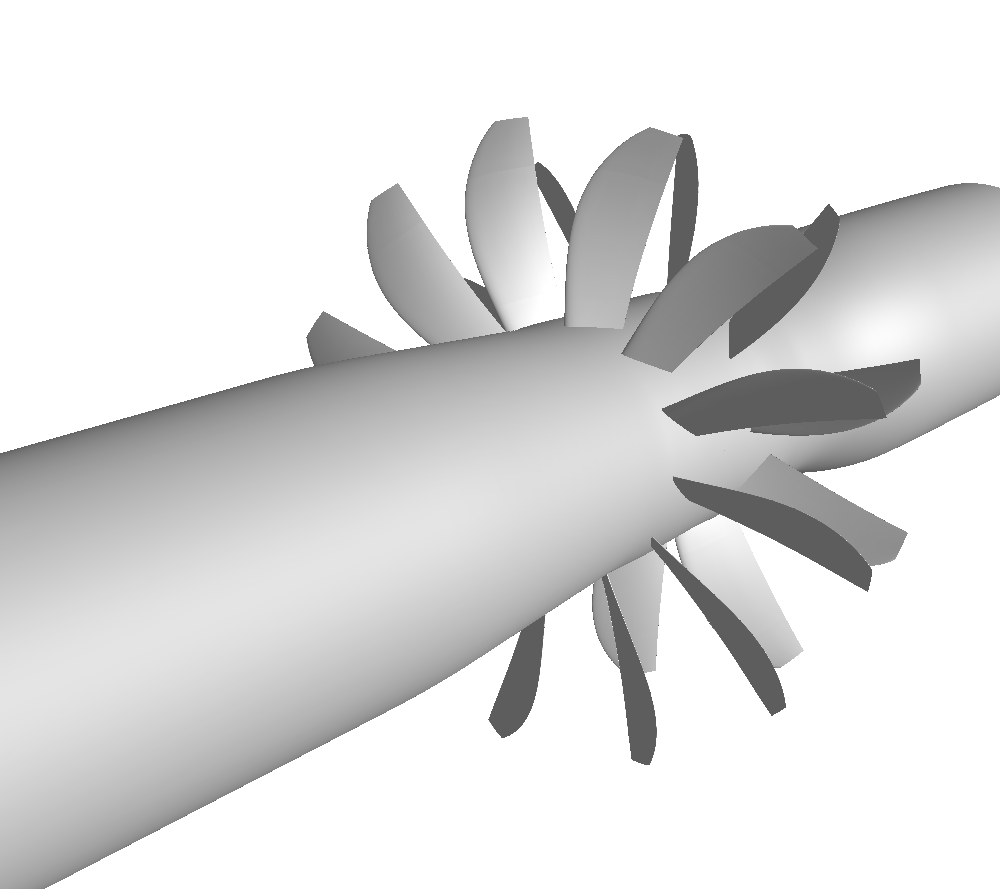
\includegraphics[width=.3\textwidth]{DREAM_LS_wall.png}
  \caption{Low-speed isolated contra-rotating open rotor geometry.}
  \label{fig:dream_ls_wall}
\end{figure}

The studied configuration is a pusher contra-rotating open rotor
that comes from the know-how of SAFRAN-Snecma. 
It is shown in Figure~\ref{fig:dream_ls_wall} for the
Low-speed (LS) flight condition, representative of the take-off
and landing.
The simulated configuration does not include the spinner as the
experimental setup does not take into account this part of the geometry.
The experimental results were not available for comparison
at the time this study was written.

\begin{table}[htp]
  \ra{1.3} \centering
  \begin{tabular}{ccc}
    \toprule
    $M_0$ & $J$ & $M_{tip}$ \\
    \midrule
    $0.2$ & 1.06 & 0.63 \\
    \bottomrule
  \end{tabular}
  \caption{Low-speed isolated contra-rotating open rotor flight condition parameters.}
  \label{tab:dream_ls_flight_condition}
\end{table} 
Table~\ref{tab:dream_ls_flight_condition} recalls the main
parameters of the case: the inflow Mach number $M_0$,
the advance ratio $J$ (see Chap.~\ref{cha:cror})
and the Mach number at the tip of
the front rotor blades based on the inflow 
velocity and the advance ratio
\begin{equation}
  \begin{split}
    M_{tip} &= 
        \sqrt{\frac{V_0^2 + (\Omega R)^2}{\gamma R t_0}} =
        \frac{V_0}{\sqrt{\gamma R t_0}} 
          \sqrt{1 + \left(\frac{\Omega R}{V_0}\right)^2} =
        \frac{V_0}{\sqrt{\gamma R t_0}} 
          \sqrt{1 + \left(\frac{\pi n D}{
          V_0}\right)^2} \\
    &= M_0 \sqrt{1 + \left(\frac{\pi}{J} \right)^2}
  \end{split}
  \label{eq:m_tip}
\end{equation}

At this flight condition, the inflow Mach 
number $M_0$ is within the incompressible range
($M_0 < 0.3$). As the CFD flow solver used here is 
\textit{elsA}~\cite{Cambier2013} CFD code which is a compressible code, 
a preconditionner might be needed for the computations to converge. 
Hopefully, the fluid is accelerated by the two rotors
and the tip Mach number is high enough not to use any preconditionning.
However, let us bare in mind that this range of Mach number might
be tedious for a compressible flow solver.
The advance ratio $J$ is around~1 which is a classical value for
low-speed propellers~\cite{Bousquet2012}. 

Two structural modes are considered for the aeroelastic study of this 
configuration: the second bending/flection mode and the first torsion mode
of the front rotor. These were inputs of the current work.
The shape of the modes is shown in Figure~\ref{fig:dream_ls_ael_modes}
with an arbitrary amplitude, large enough to ease the visualization.
Two inflection lines are seen for the 2F mode, while only
one is seen for the 1T, hence their designation.
\begin{figure}[htp]
  \centering
  \subfigure[2F]{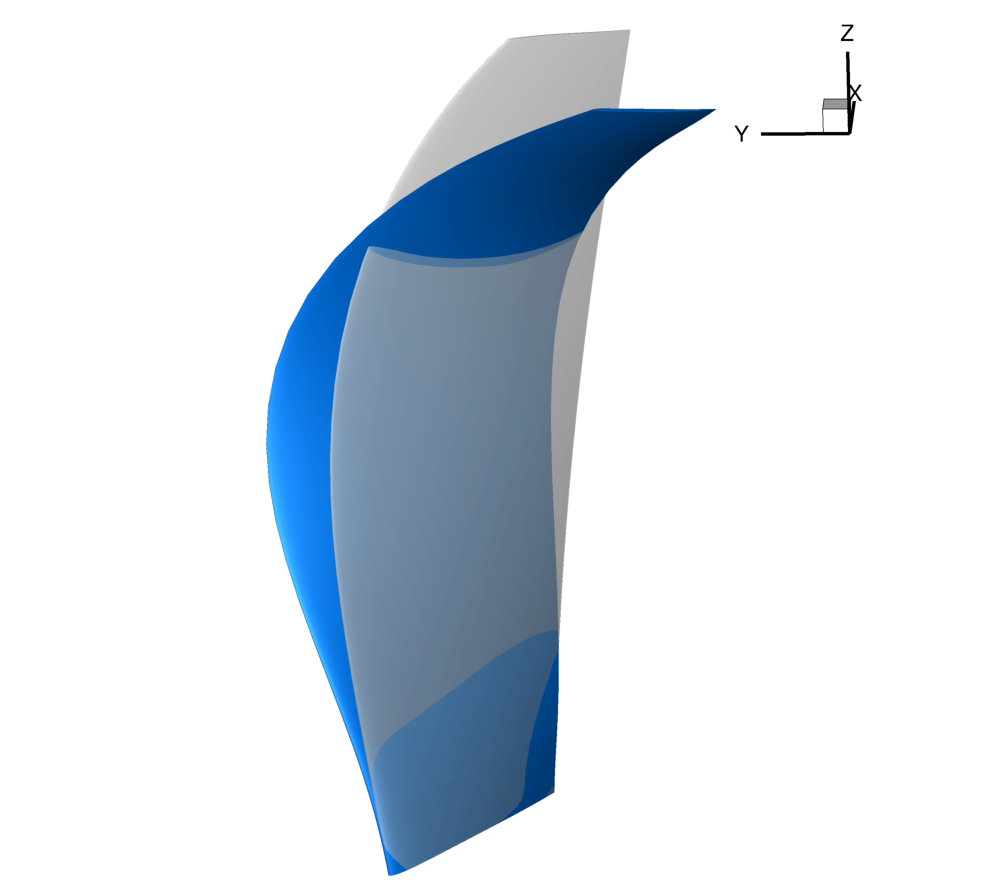
\includegraphics[height=.35\textwidth]{mode_2F.png}}
  \subfigure[1T]{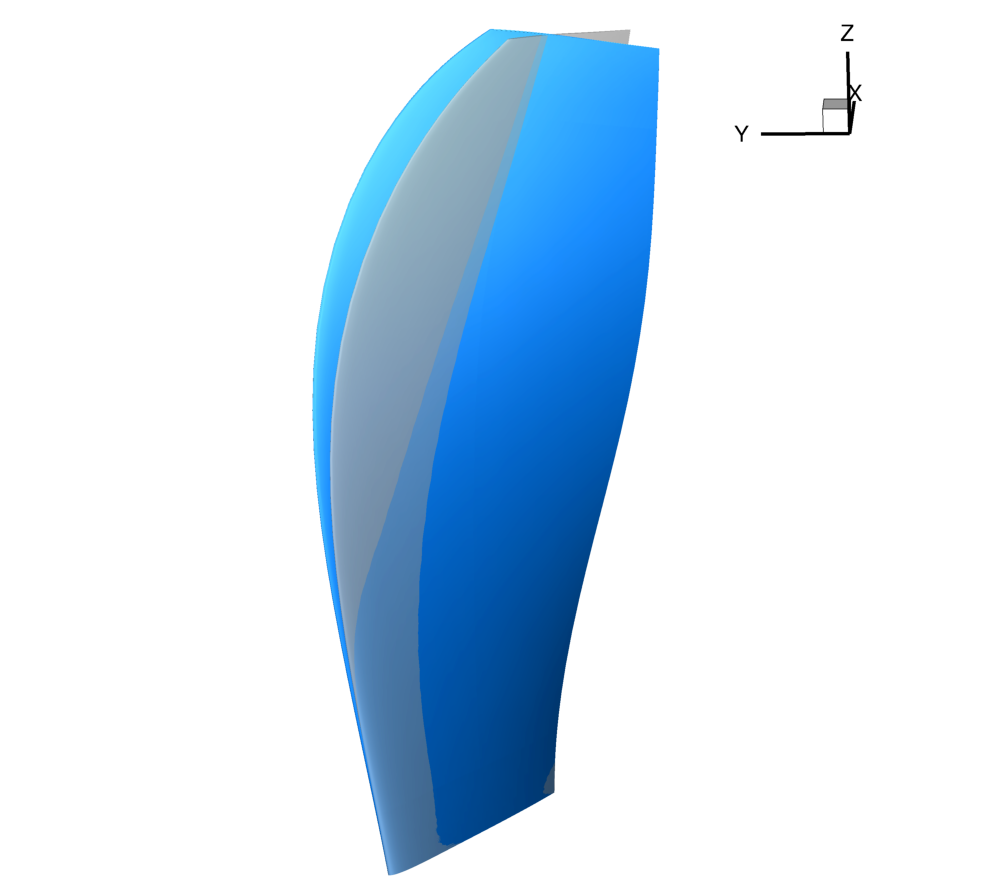
\includegraphics[height=.35\textwidth]{mode_1T.png}}
  \caption{Low-speed isolated configuration: structural modes considered.}
  \label{fig:dream_ls_ael_modes}
\end{figure}
The frequency, mass and stiffness of the modes 
are given with the corresponding modes.
The ratio of the frequency of the blade passing 
frequency of the opposite row, namely the rear rotor,
and the aeroelastic frequency of
each mode vary between 
$3.19 \leq f_{BPF} / f_{AEL} \leq 3.87$. However,
this last frequency governs the unsteady rigid flow physics 
and will have to be computed along with the aeroleastic frequency.
Therefore, the multi-frequential formulation of the
harmonic balance approach will be used to simulate the
aeroelastic response of the blades (see Sec.~\ref{sec:dream_ls_ael_results}).


\section{Numerical setup}
\label{sec:dream_ls_numerical}
%!TEX root = ../../../adrien_gomar_phd.tex

The mesh considered to compute this
CROR configuration is a single-blade passage meshed
with an O4H topology show in Fig.~\ref{fig:dream_mesh}. This is a classical
topology for turbomachinery computations that is here applied to 
a CROR.
\begin{figure}[htb]
  \centering
  \subfigure[Mesh topology]{
    \label{fig:dream_mesh}
    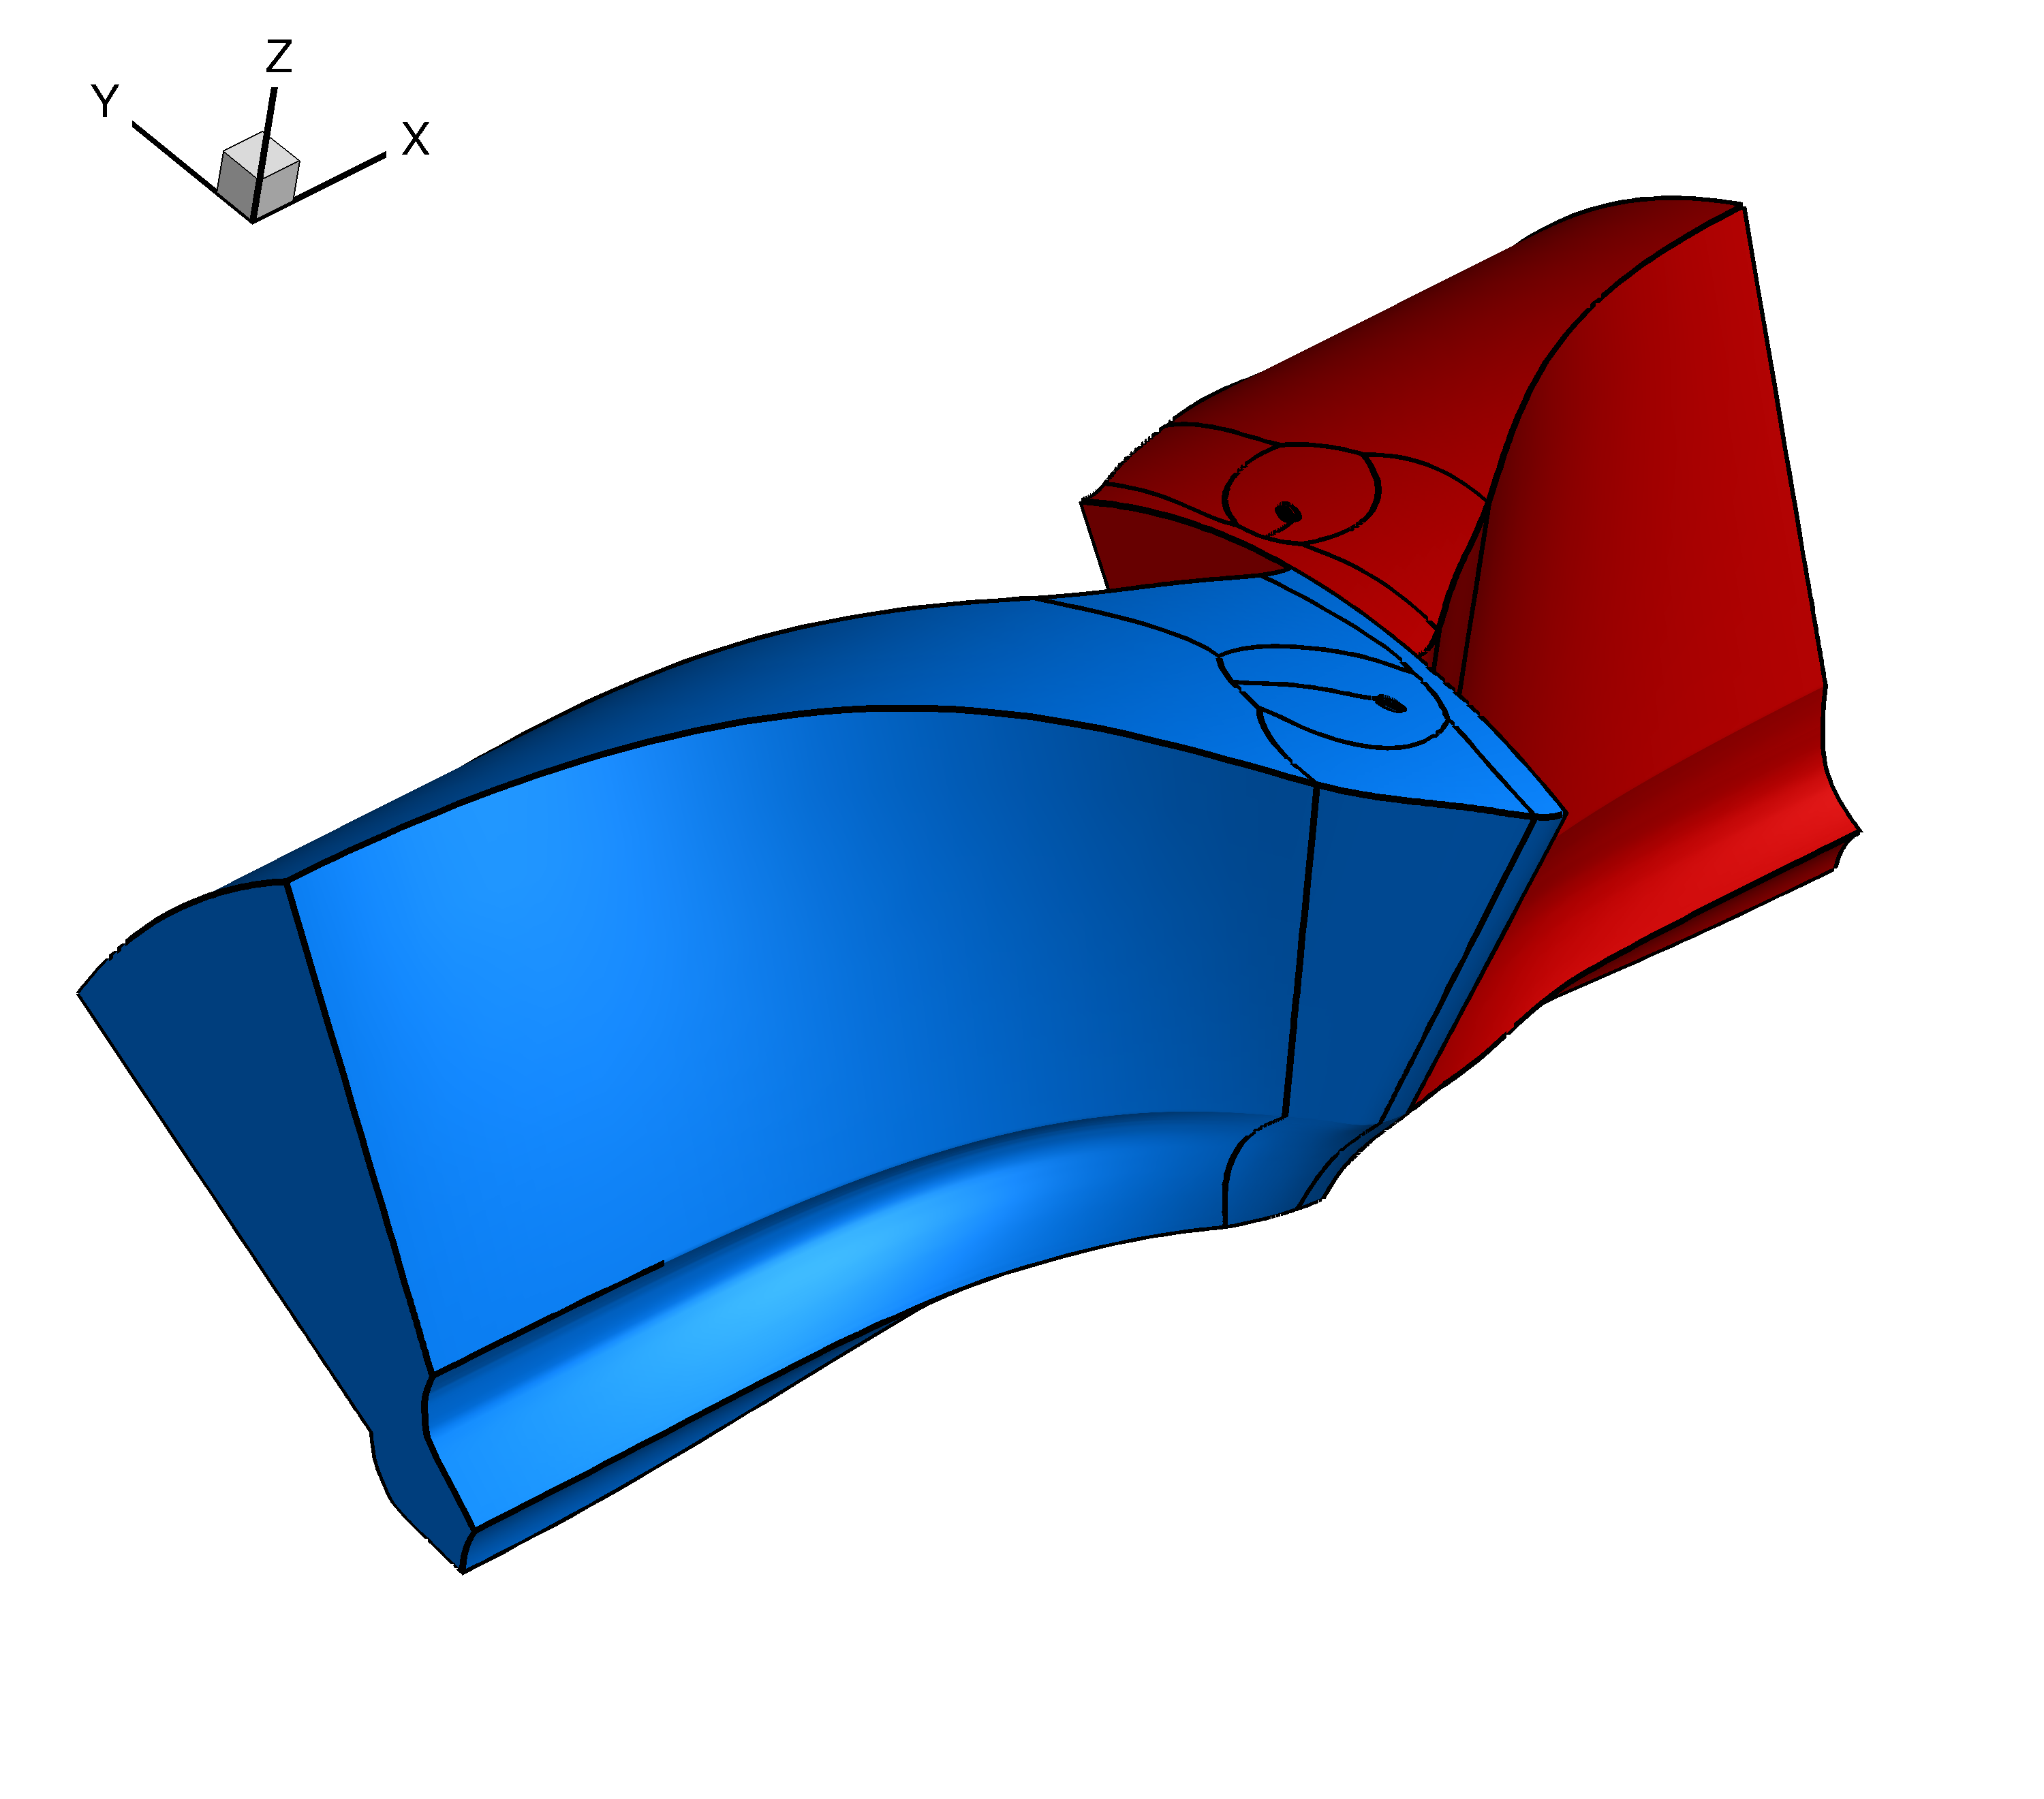
\includegraphics[width=.4\textwidth]{dream_mesh.png}}
  \subfigure[Far-field domain]{
    \label{fig:dream_farfield}
    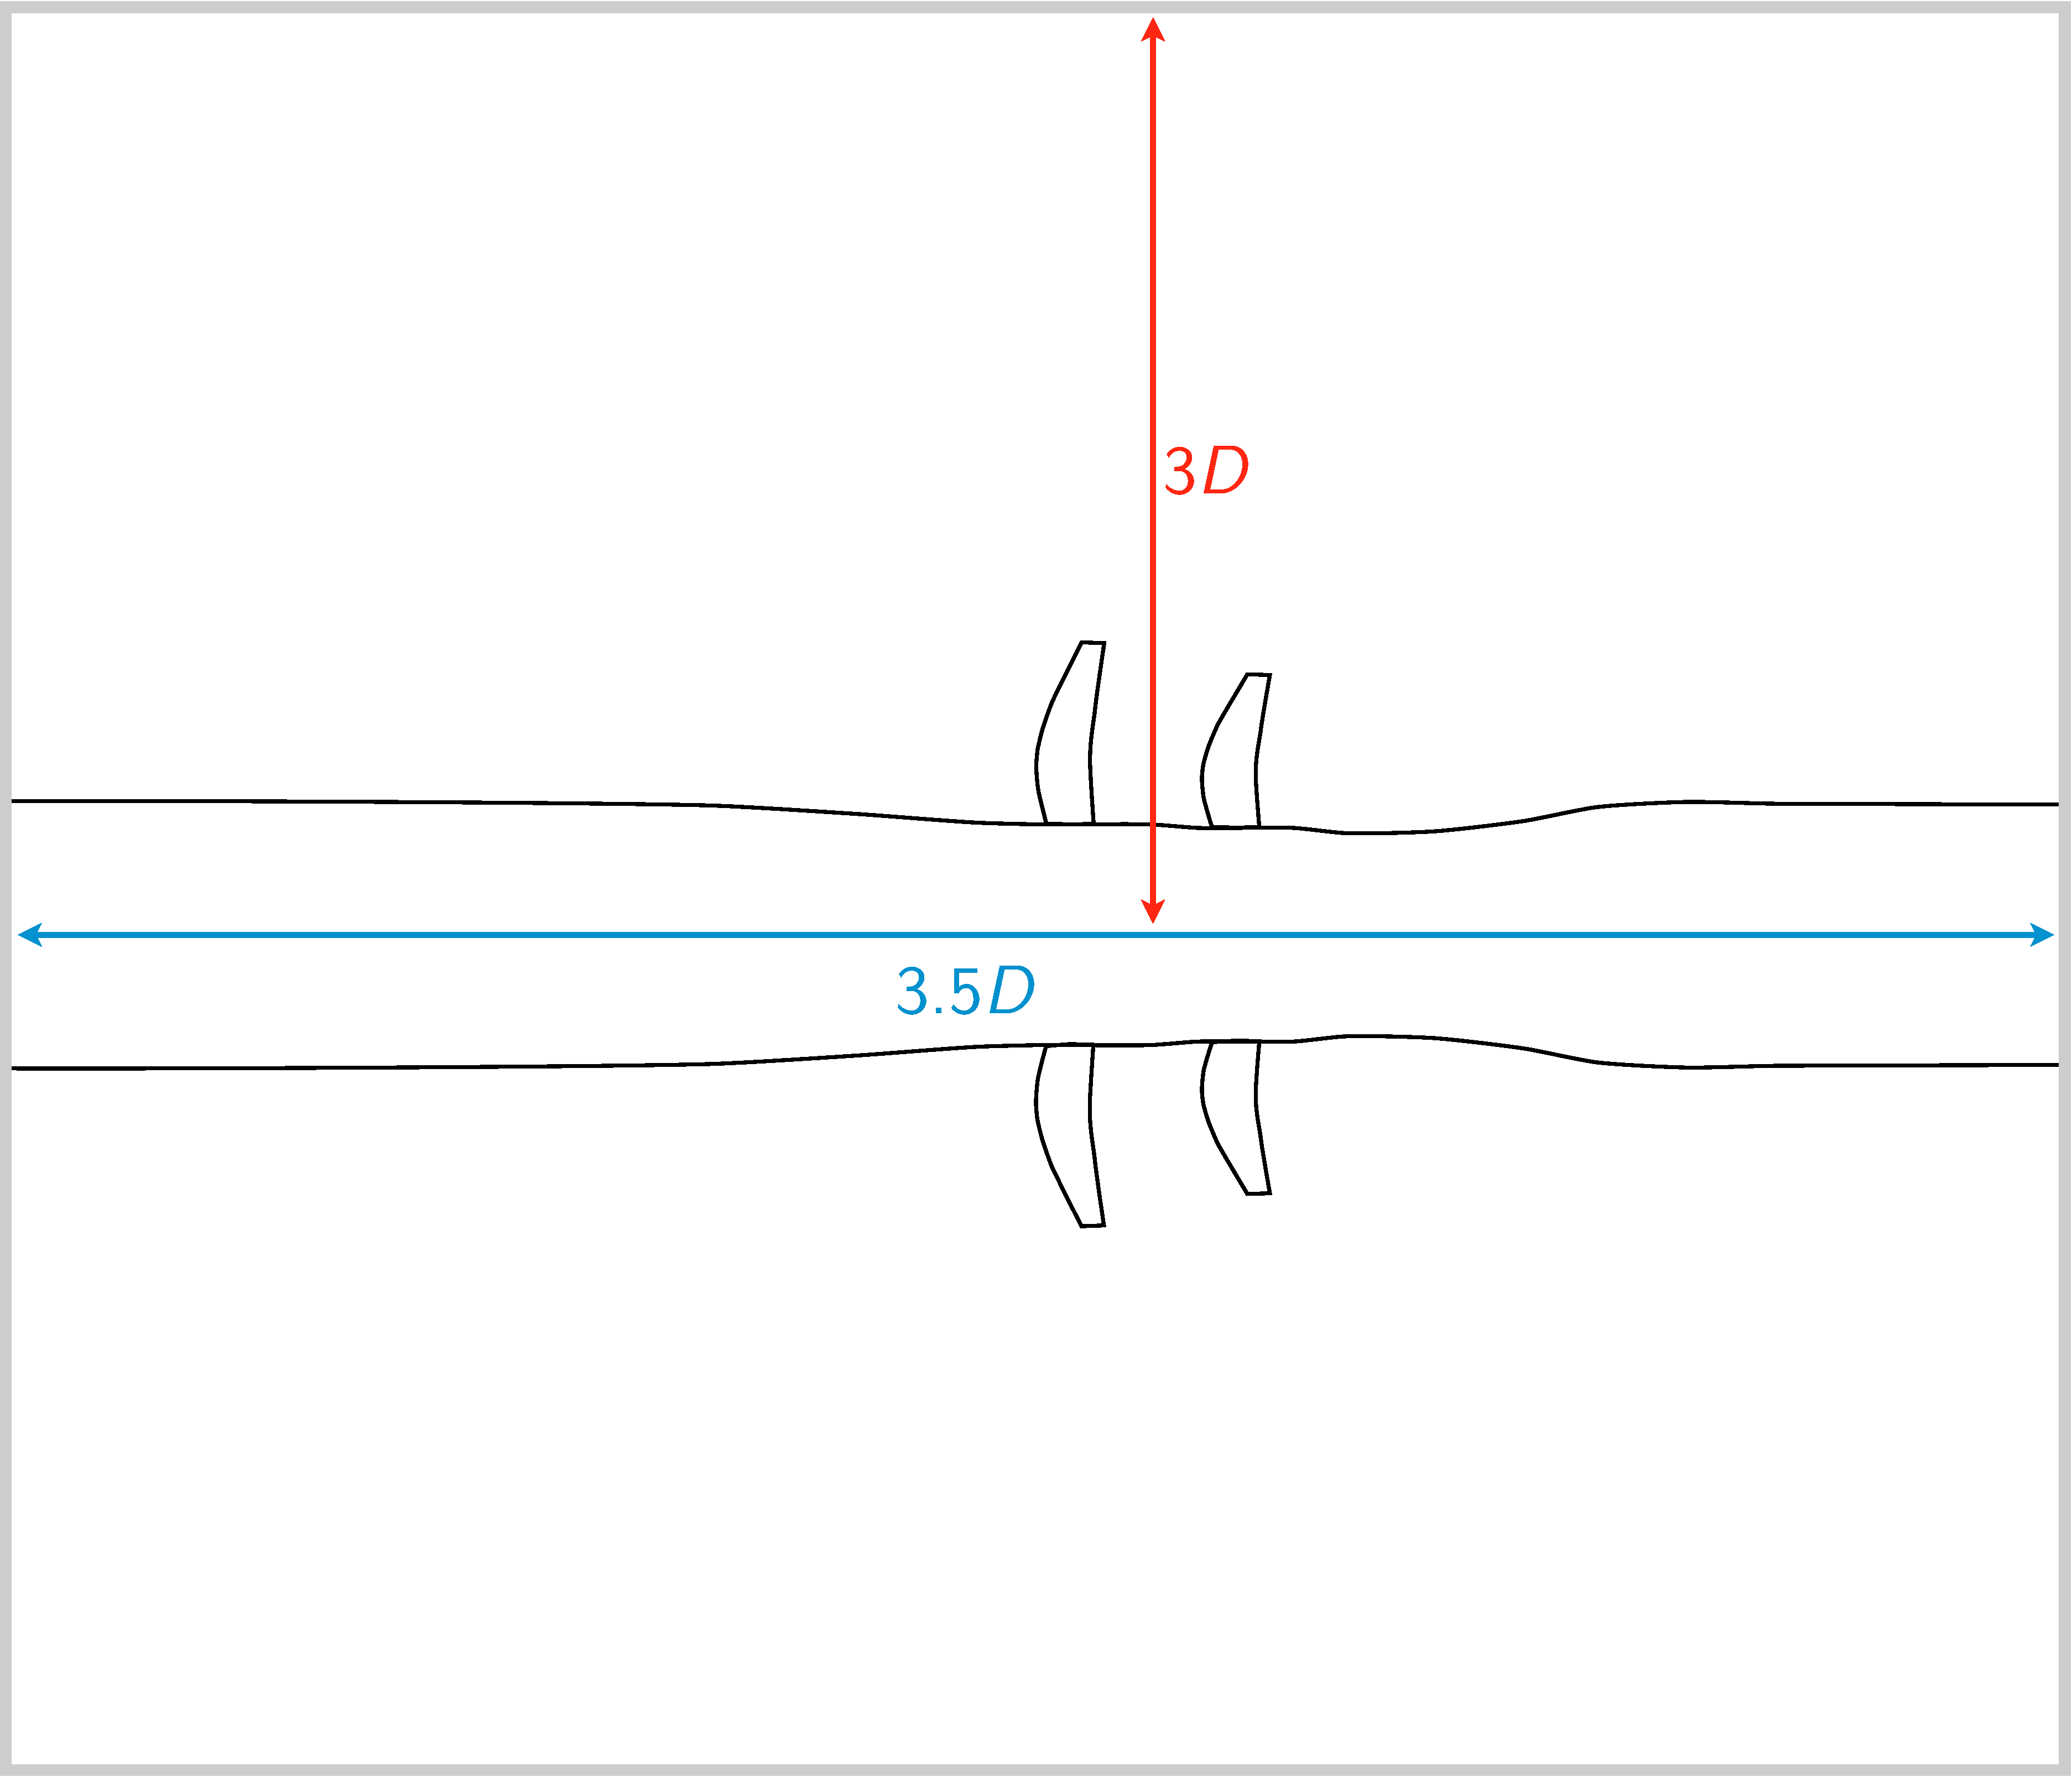
\includegraphics[width=.4\textwidth]{dream_farfield.pdf}}
  \caption{Computational domain considered.}
\end{figure}

As this last is not shrouded, a sufficiently large
far-field domain is taken to ensure a minimum influence
of the boundary conditions.
The computational domain is shown in Fig.~\ref{fig:dream_farfield}.
The radial extent is $3D$ while the axial one is $3.5D$.
\citet{Peters2012} consider an axial extent of $7.5D$
with a radial extent of $4D$ while \citet{Zachariadis2011}
consider $2.5D$ and $3.6D$, respectively. We are thus in 
the mid-range of the values taken in the literature.

As highlighted by underlined text in Fig.~\ref{fig:dream_farfield},
the boundary conditions used are: (i)~adiabatic walls
for the blades and the shroud (or spinner) and (ii)~constant
stagnation values used at the far-field.

Turbulence is modeled using the one-equation model of
\citet{Spalart1992}.  Roe's scheme~\cite{Roe1981} along with a 
second-order MUSL extrapolation 
is used to compute the convective fluxes.
The maximum CFL number is set to~10 for the steady 
computations and the HB simulations.


\section{Steady results}
\label{sec:dream_ls_steady_results}
%!TEX root = ../../../adrien_gomar_phd.tex

\subsection{Convergence analysis}
\label{sub:dream_ls_conv_coeff}

Convergence of the steady computation using the Roe~2 space scheme
is reported in Figure~\ref{fig:dream_ls_convergence_roe2}. The residuals
show a four orders of magnitude decrease and the similarity
coefficients are stable starting at 500~iterations.
Therefore, according to \citet{Casey2000}, the
solution is considered to be converged.
\begin{figure}[htp]
  \centering
  \subfigure[residuals]{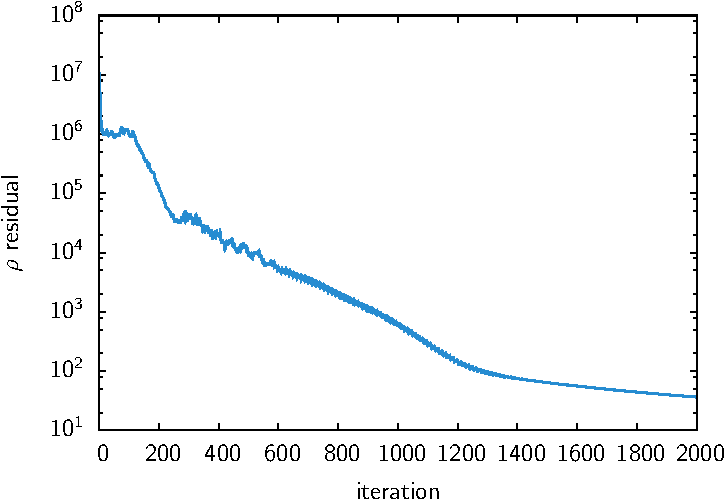
\includegraphics[width=.35\textwidth]{DREAM_LS_RESIDUALS_PPT.pdf}}
  \subfigure[thrust coefficient]{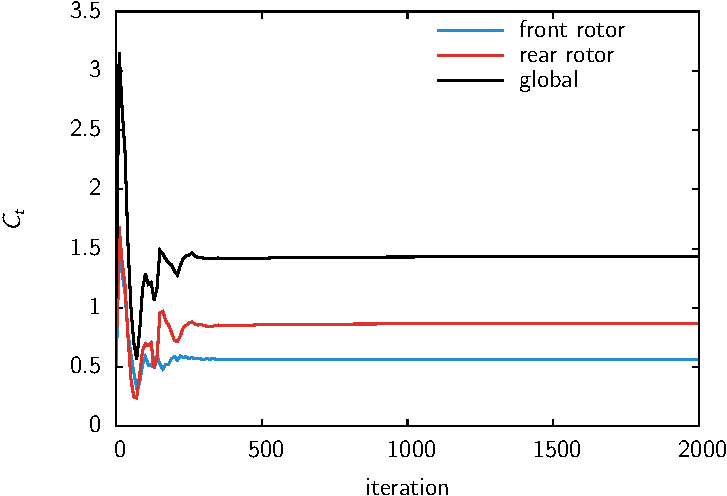
\includegraphics[width=.35\textwidth]{DREAM_LS_FORCES_CT_PPT.pdf}}
  \subfigure[power coefficient]{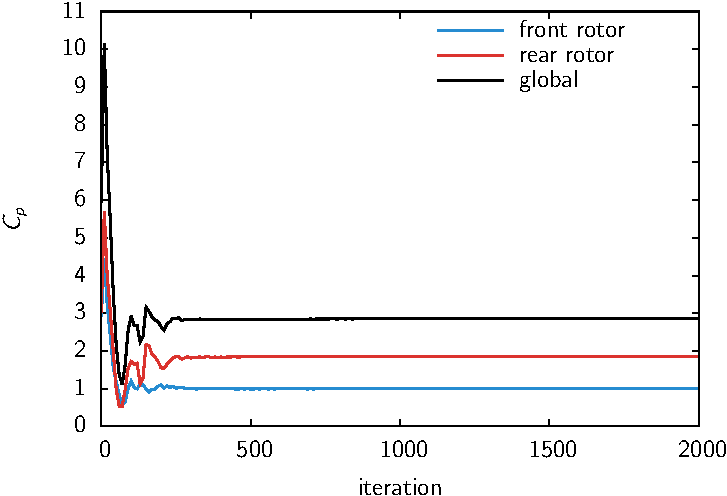
\includegraphics[width=.35\textwidth]{DREAM_LS_FORCES_CP_PPT.pdf}}
  \subfigure[efficiency]{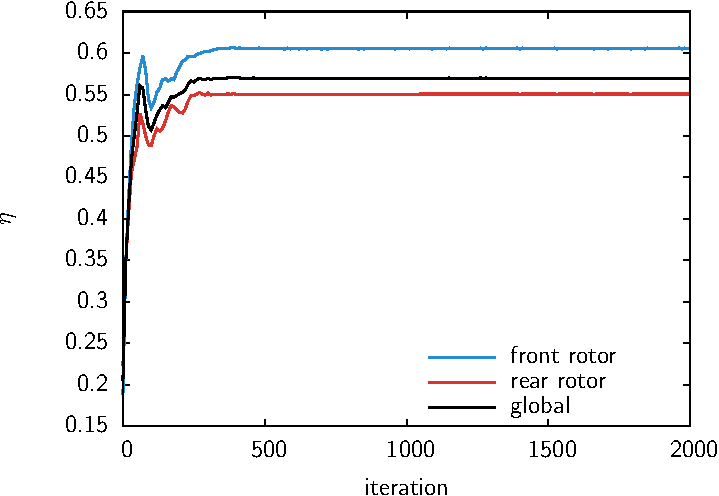
\includegraphics[width=.35\textwidth]{DREAM_LS_FORCES_ETA_PPT.pdf}}
  \caption{Low-speed isolated configuration: convergence of the Roe~2 steady
  computation.}
  \label{fig:dream_ls_convergence_roe2}
\end{figure}

\subsection{Similarity coefficients}
\label{sub:dream_ls_sim_coeff}

The similarity coefficients (defined in 
Sec.~\ref{sub:cror_similarity_coeff}) are post-processed 
and reported in Tab.~\ref{tab:dream_ls_sim_coeff}.
\begin{table}[htp]
  \ra{1.3} \centering
  \begin{tabular}{ccc||ccc|ccc}
    \toprule
     \multicolumn{3}{c||}{global} & \multicolumn{3}{c|}{front} & \multicolumn{3}{c}{rear} \\
    $C_T$ & $C_P$ & $\eta$ & $C_{T_f}$ & $C_{P_f}$ & $\eta_f$ & $C_{T_r}$ & $C_{P_r}$ & $\eta_r$ \\
    \midrule
    1.132 & 2.093 & 0.573 & 0.564 & 0.994 &  0.600 & 0.568 & 1.099 &  0.548 \\
    \bottomrule
  \end{tabular}
  \caption{Low-speed isolated configuration: similarity coefficients.}
  \label{tab:dream_ls_sim_coeff}
\end{table}
The results are consistent with the efficiency estimation given in 
Eq.~\eqref{eq:estimation_sim_coeff} for a propeller at take-off flight conditions.
In fact, each rotor of the CROR has an efficiency that is between $0.5$
and $0.6$. The advantage of the CROR is demonstrated here as the rear
rotor is able to retrieve an additional thrust coefficient of $0.568$ yielding
a total of $1.132$, while
the front rotor alone would only give $0.564$.
The presence of a second rotor allows to more than double 
the total thrust of the engine. 
Nevertheless, the efficiency is affected compared to a single row 
propeller, as
it goes from $0.600$ for the front rotor alone to $0.573$ for the CROR.
However, achieving such a level of thrust coefficient ($C_T = 1.132$)
with an isolated
propeller would require a higher loading of the blades which is not
consistent with an increase of the efficiency, necessary to meet the ACARE goals.
Actually, this is the main advantage 
of the CROR engine: two rotors are used to create the thrust which allows to
reduce the loading of each rotor compare to an isolated propeller,
allowing thus higher inflow Mach numbers. In fact, the rotation of the rotors is reduced 
to maintain a subsonic Mach number optimizing thus the efficiency
for a given level of thrust. Moreover, by maintaining a subsonic
Mach number, the noise emissions are retained.

\subsection{One-dimensional results: radial profiles}
\label{sub:dream_ls_radial_profiles}

Radial profiles positioned at six locations upstream and downstream the rotors
are extracted and shown in Figure~\ref{fig:dream_ls_position_radial}.
The absolute
Mach number, absolute flow angle, static pressure, 
stagnation temperature and stagnation pressure
are shown in Figure~\ref{fig:dream_ls_radial_profiles}
against the radial position expressed
relative to the radius of the front rotor blade $R_f$.

The absolute Mach number, shown in 
Figure~\ref{fig:dream_ls_radial_profiles_ma}, is increased by
the two rotors as it goes from the inflow condition value $M=0.2$
up to $M=0.4$. Note that above $R/R_f=1$, namely at the tip
of the front rotor blade, the Mach number
almost recovers the inflow condition. Moreover, it can be inferred from the
absolute Mach number radial evolution, that the stream tube is contracting which is consistent
with the observed acceleration of the fluid.

The pitch angle of the absolute velocity vector is shown in 
Figure~\ref{fig:dream_ls_radial_profiles_alpha}. The front rotor
deviates the flow of almost $20^\circ$, justifying the need
for a second rotor. Between the fourth and the fifth extraction planes, namely
passing through the rear rotor, the flow is straighten up. Remember that 
the very first motivation for adding a second rotor to a propeller
was to recover the energy lost by the swirling flow
(recall Sec.~\ref{sub:cror_velocity_triangle}). This is observed in our simulations as
the deflection angle is now close to $0^\circ$ for $0.3 \leq R/R_f \leq 0.7$
in plane $P6$.
Below that, the deflection angle remains negative. In the tip vortex region
of the rear rotor, one can see the effect of the two tip vortices: between 
$0.8 \leq R/R_f \leq 0.9$, the front rotor tip vortex is seen as the 
deflection angle is positive while between $0.7 \leq R/R_f \leq 0.8$
the rear rotor is observed, 
which is consistent with the positive
peak observe near the blade tip region in planes $P3$ and $P4$.

The goal of a CROR is to create thrust through an acceleration of 
the flow rather than to produce static pressure as in a compressor stage.
This is highlighted in Figure~\ref{fig:dream_ls_radial_profiles_ps}
where the static pressure increases by at-most 2\% which has to 
be compared with an almost 100\% increase of the absolute
Mach number. This is consistent with the low inflow Mach number
that is with the incompressible range.
A small increase is observed at each
rotor crossing. Upstream the rotors, the potential effects can
be seen. Actually, the flow is accelerated by the rotors, this acceleration
yields a decrease of the static pressure 
(roughly through the Bernouilli theorem) and this pressure deficit is observed in
planes $P1$, $P2$ and $P4$.

Figure~\ref{fig:dream_ls_radial_profiles_ti}
shows the stagnation temperature.
An increase is observed at each 
rotor crossing. This is consistent as
a propeller row gives work to the fluid. As such,
the first principle of thermodynamics states that the 
enthalpy will raise resulting in an increasing stagnation
temperature observed in our results. One can observe that
the enthalpy increase is greater on the rear rotor compared
to the front rotor.

The stagnation pressure evolution is shown in 
Figure~\ref{fig:dream_ls_radial_profiles_pi}. As the static pressure
and the absolute Mach number increases along with the crossing of the rotors,
it is logical to have an increase of the stagnation pressure.
\begin{figure}[htp]
  \centering
  \subfigure[position of the extraction planes]{
    \label{fig:dream_ls_position_radial}
    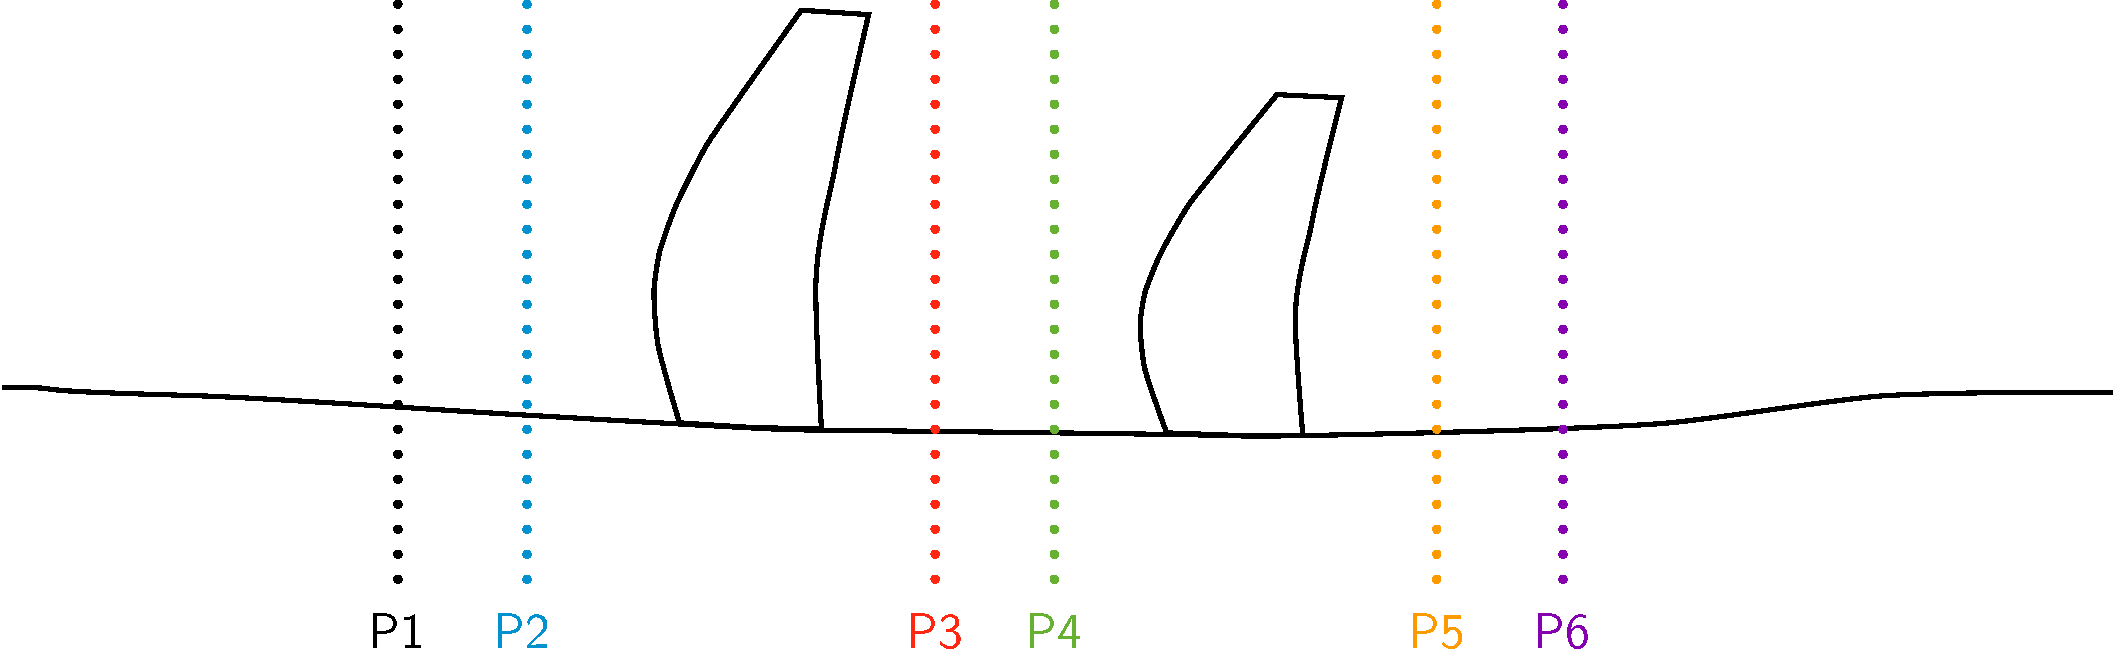
\includegraphics[width=.55\textwidth]{dream_position_azi_mean.pdf}}
  \subfigure[absolute Mach number]{
    \label{fig:dream_ls_radial_profiles_ma}
    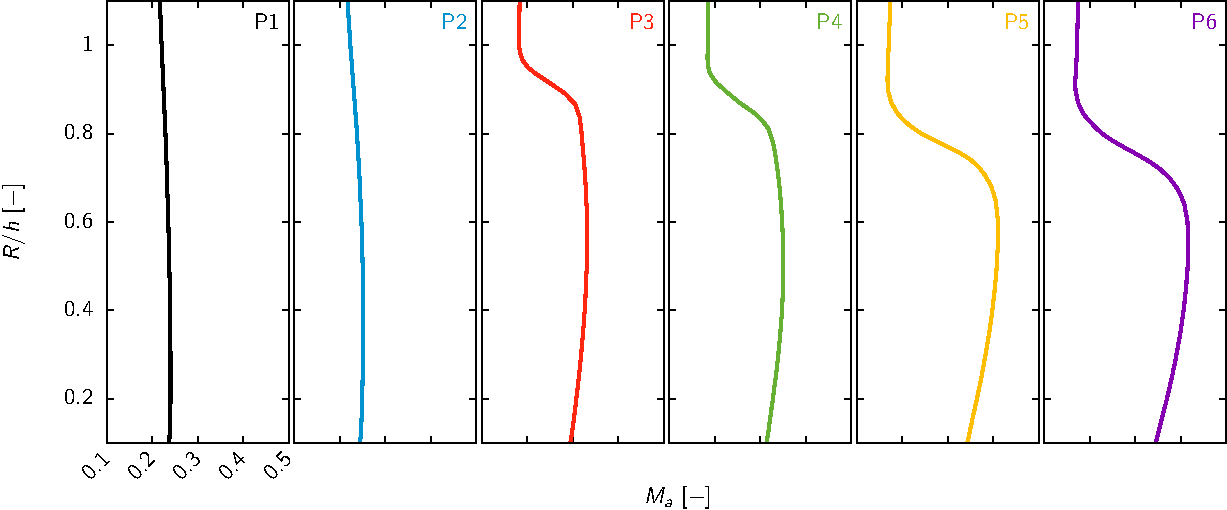
\includegraphics[width=.72\textwidth]{DREAM_LS_RANS_AZI_MEAN_PPT_macha.pdf}}
  \subfigure[absolute flow angle]{
    \label{fig:dream_ls_radial_profiles_alpha}
    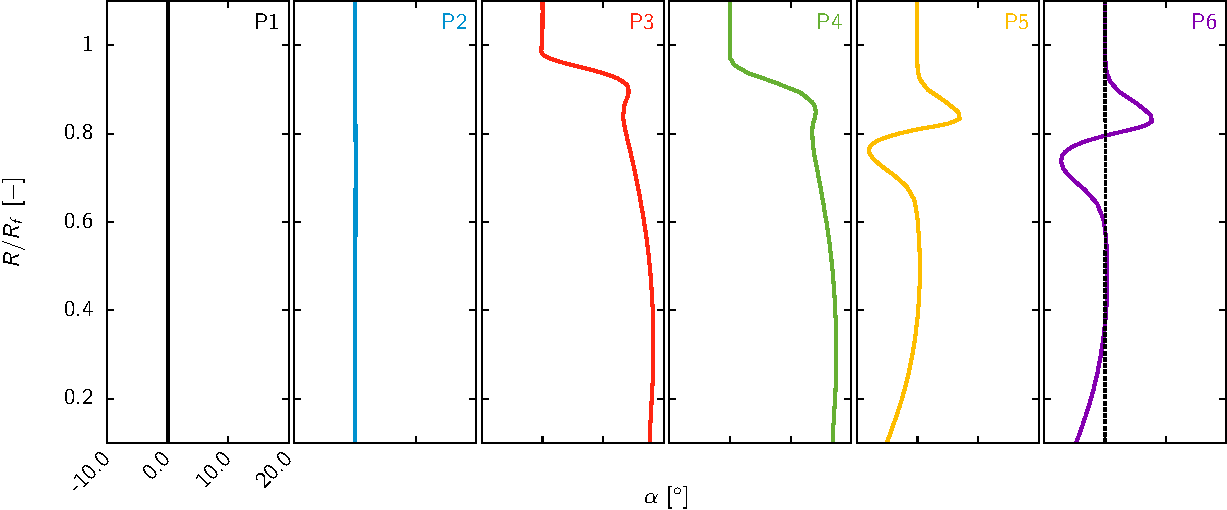
\includegraphics[width=.72\textwidth]{DREAM_LS_RANS_AZI_MEAN_PPT_alpha.pdf}}
  \caption{Low-speed isolated configuration: radial profiles.}
\end{figure}
\setcounter{figure}{\value{figure}-1}
\begin{figure}[htp]
  \centering
  \setcounter{subfigure}{3}
  \subfigure[static pressure]{
    \label{fig:dream_ls_radial_profiles_ps}
    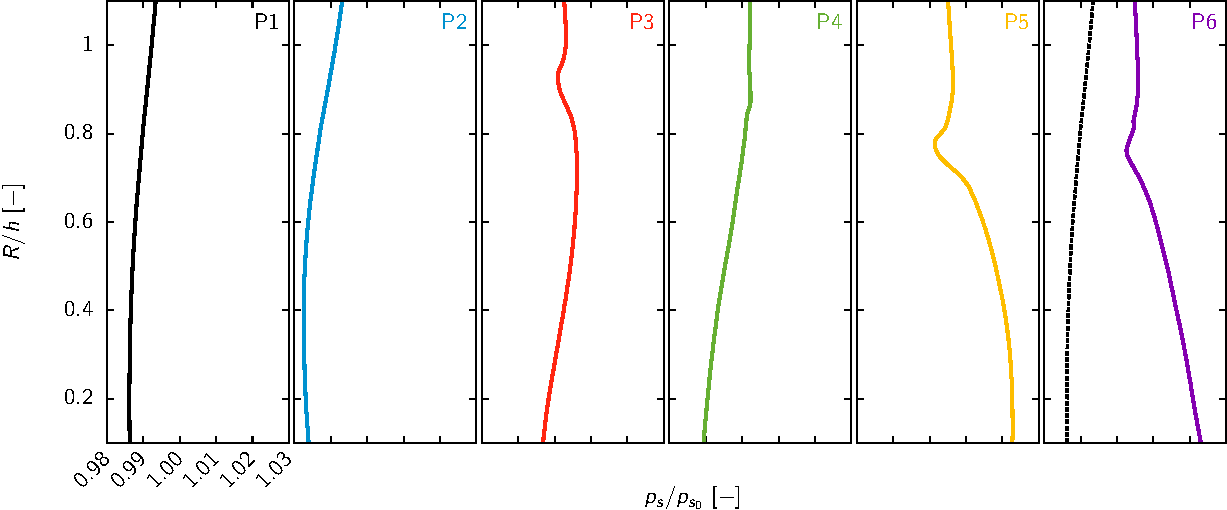
\includegraphics[width=.72\textwidth]{DREAM_LS_RANS_AZI_MEAN_PPT_ps.pdf}}
  \subfigure[stagnation temperature]{
    \label{fig:dream_ls_radial_profiles_ti}
    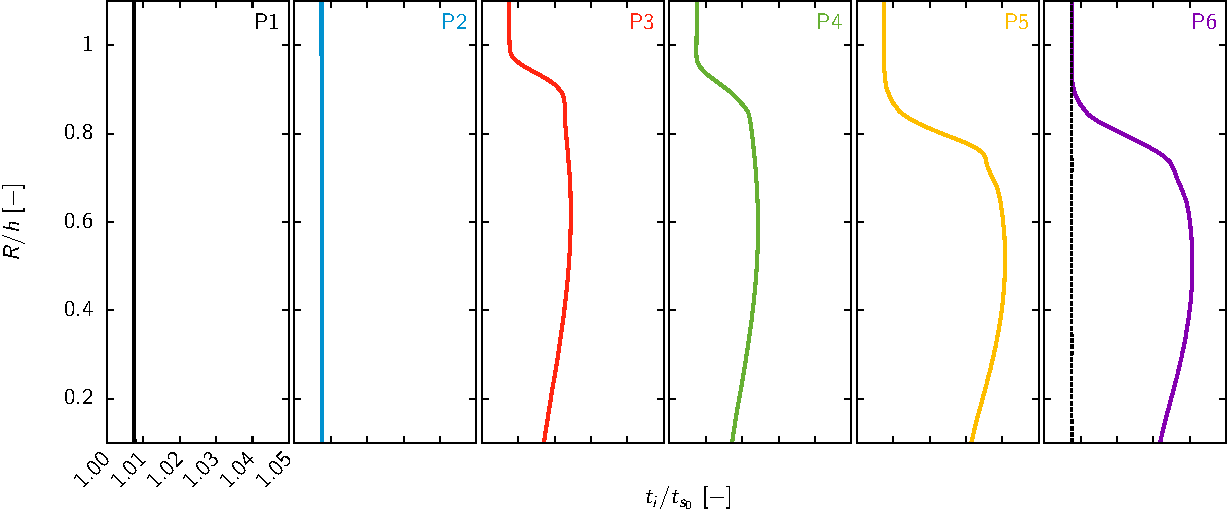
\includegraphics[width=.72\textwidth]{DREAM_LS_RANS_AZI_MEAN_PPT_ti.pdf}}
  \subfigure[stagnation pressure]{
    \label{fig:dream_ls_radial_profiles_pi}
    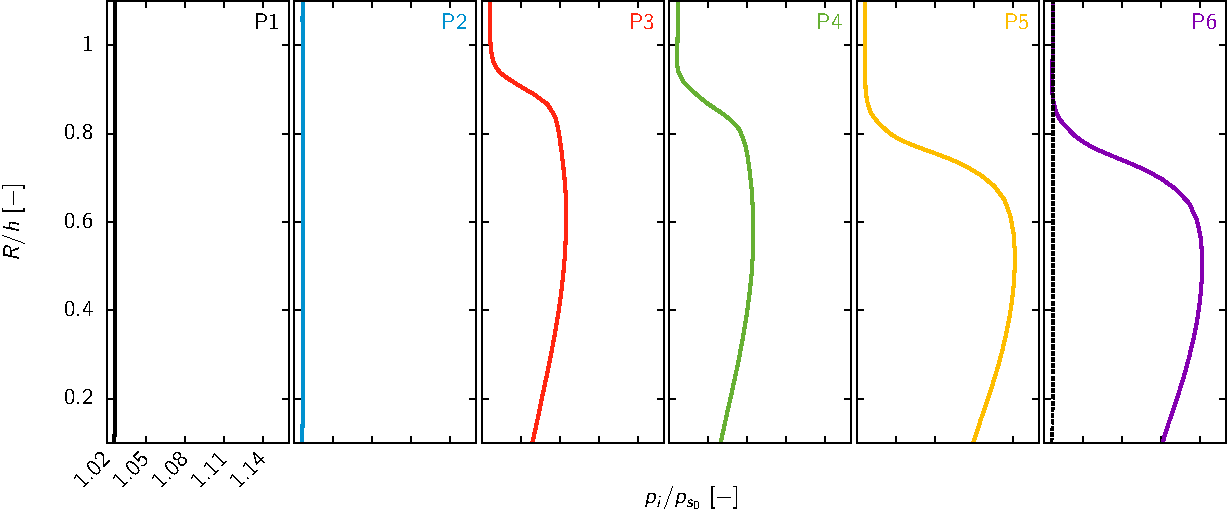
\includegraphics[width=.72\textwidth]{DREAM_LS_RANS_AZI_MEAN_PPT_pi.pdf}}
  \caption{Low-speed isolated configuration: radial profiles (contd.).}
  \label{fig:dream_ls_radial_profiles}
\end{figure}

These 1D results provide us confidence in our simulation. 
In fact, the flow physic that
was expected is observed in the results. To further analyze the simulation,
2D results are presented in the following section.

\subsection{Two dimensional results: radial and axial cuts}
\label{sub:dream_ls_flow_field}

Contours of the relative Mach number are shown in 
Figure~\ref{fig:dream_ls_mach_kp} along with the pressure coefficient $k_p$,
for both the front and the rear rotor, defined as
\begin{equation}
   k_p = \frac{p_s - p_{s_0}}{\rho n^2 D^2},
\end{equation}
where the $n$ and $D$ parameters are the one of the front rotor
to ease the comparison.

The negative $k_p$ range is attributed
to the suction side and the positive to the pressure side.
The $k_p$ should be interpreted as follow, a decreasing $k_p$
means that the pressure gradient is negative, namely the flow
is accelerating.
Classically, the $k_p$ axis is reversed so that the suction side
is on top of the figure and the suction side on bottom.
The stagnation point is highlighted
by the maximum of the pressure coefficient. On the pressure side 
($k_p > 0$) the flow accelerates
toward the trailing edge with a favorable pressure gradient. 
On the suction side, a rapid acceleration of the fluid
is observed near the leading edge 
($\partial k_p / \partial x \ll 0$) followed by
a deceleration of the fluid along with an
adverse pressure gradient.
On the front rotor, the integrated pressure coefficient is
increasing along with the relative span, at least 
when comparing the 50~\% and the 75~\% relative spans.
After that, the pressure coefficient is almost constant on 
the front rotor. The loading is thus almost constant for
relative spans greater than 50~\%. 
% In the propeller community and
% by extension the CROR community, the loading of a blade is known
% to be maximal for a relative span of 75~\%~\cite{Bousquet2012},
% which is consistent with our results.

The pressure coefficients on the rear rotor have a similar shape
compared to the one of the front rotor. However, the loading is
larger on the rear rotor and near the tip of the blade
$R/R_f > 75~\%$, the integrated value of the pressure coefficient
increases drastically. This is highlighted by the thrust coefficient 
of the rear rotor $C_{T_r}$ which is reported in 
Tab.~\ref{tab:dream_ls_sim_coeff} and that is higher than
the front rotor one. This is observed even though the diameter of the front
rotor is chosen to normalize the pressure coefficient which
lessened the thrust coefficient of the rear rotor.

Relative Mach number contours are also shown in 
Figure~\ref{fig:dream_ls_mach_kp}.
As inferred by the tip Mach number value $M_{tip}$ of the blade
given in Tab.~\ref{tab:dream_ls_flight_condition},
the relative Mach number does not 
cross the sonic boundary $M_{rel} = 1$.
The flow remains subsonic which is, aerodynamically speaking,
a good feature for the performances since shocks create losses.
Near the tip region of the rear rotor blades, the leaving of
the tip vortex can be seen. In fact, for relative span $R/R_f \geq 90\%$,
a low velocity region is seen on the rear rotor blades
oriented from the pressure side to the suction side direction,
hence the consistence with a tip vortex.
\begin{figure}[htp]
 \centering
 \begin{tabular}{rccc}
   & $k_p$ front rotor
   & $k_p$ rear rotor
   & relative Mach number\\
   \rotatebox{90}{\qquad\qquad 25~\%} 
   & 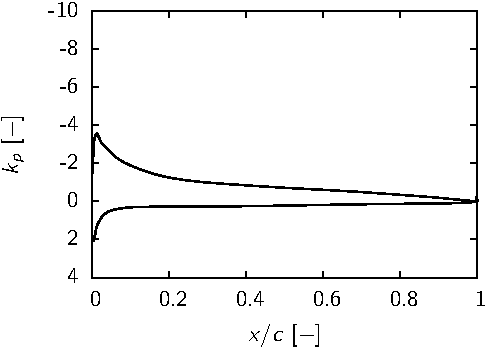
\includegraphics[width=0.28\textwidth]{DREAM_LS_KP_25_FRONT_PPT.pdf}
   & 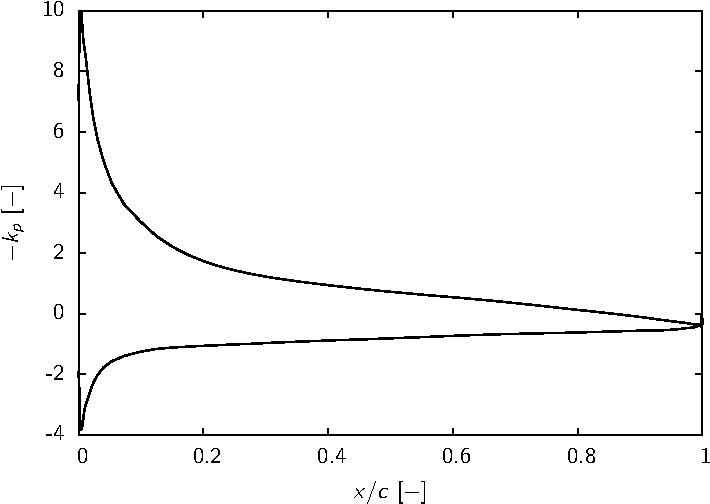
\includegraphics[width=0.28\textwidth]{DREAM_LS_KP_25_REAR_PPT.pdf}
   & 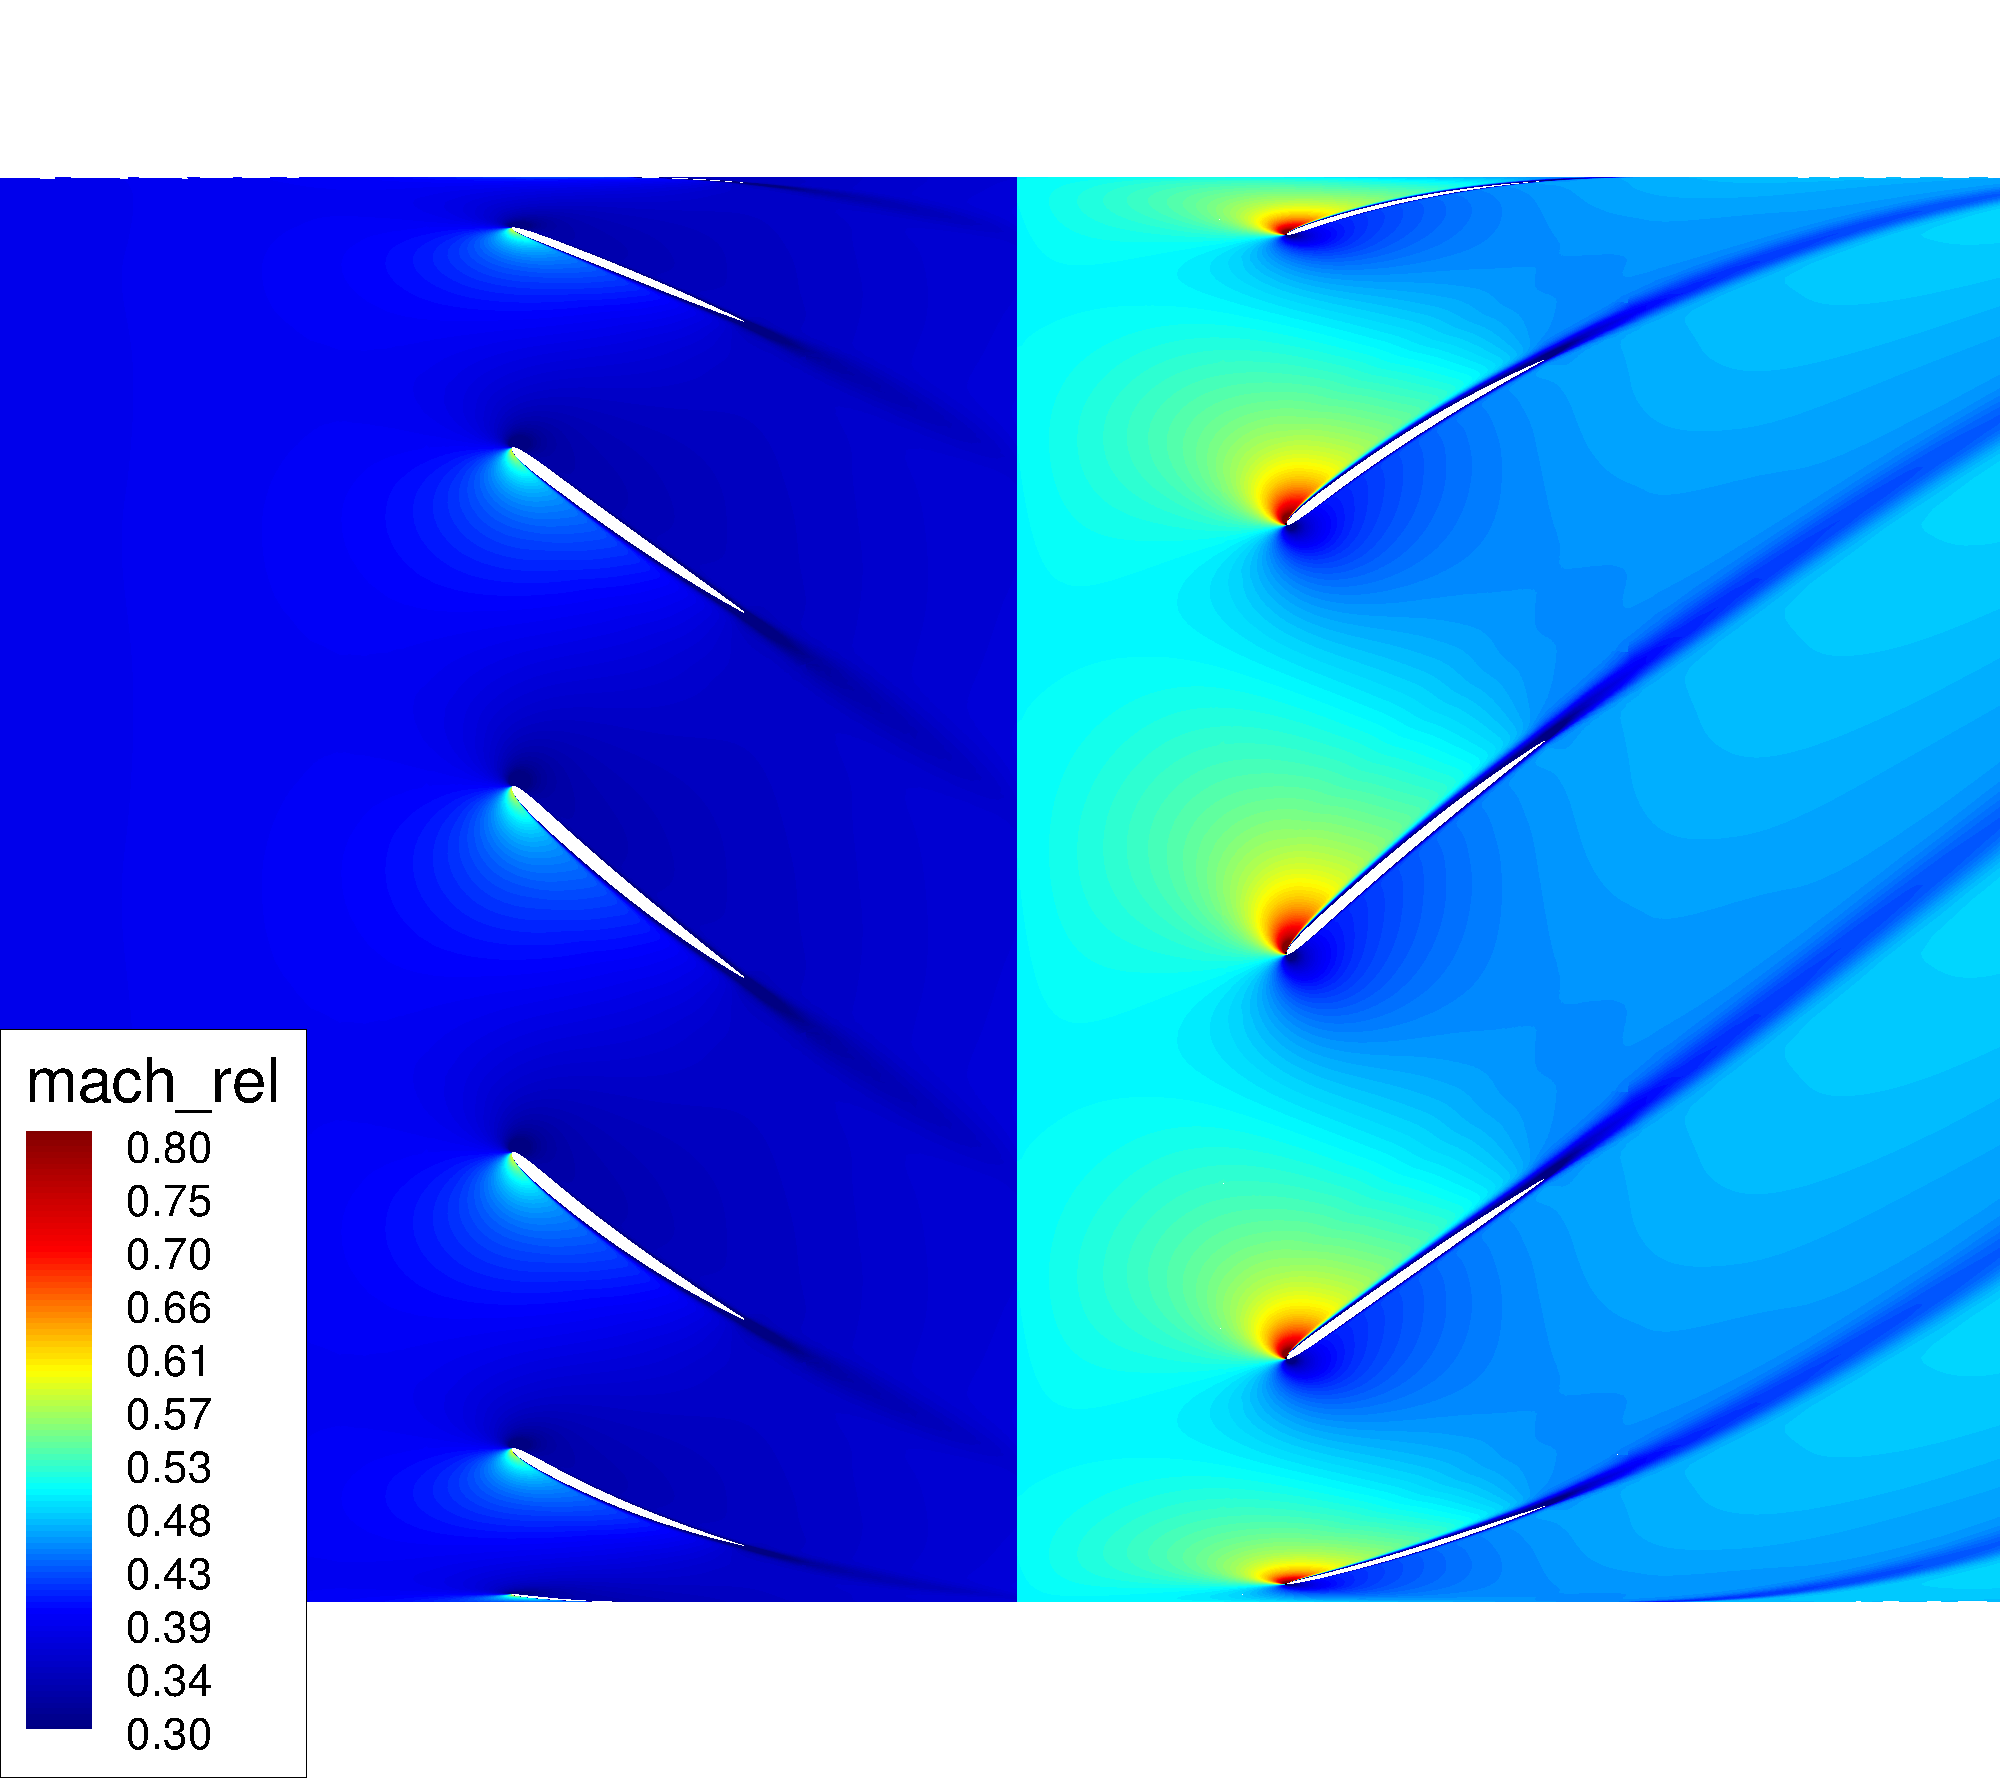
\includegraphics[width=0.28\textwidth]{DREAM_LS_RANS_roe2_sa_slice_r_25_mach_rel.png}\\
   \rotatebox{90}{\qquad\qquad 50~\%} 
   & 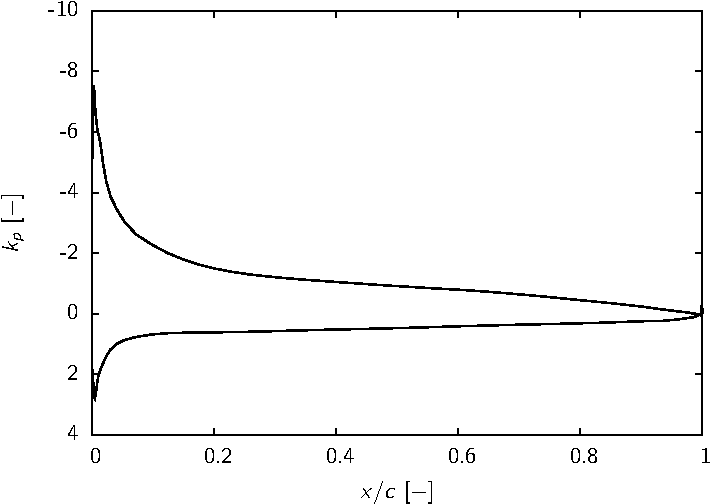
\includegraphics[width=0.28\textwidth]{DREAM_LS_KP_50_FRONT_PPT.pdf}
   & 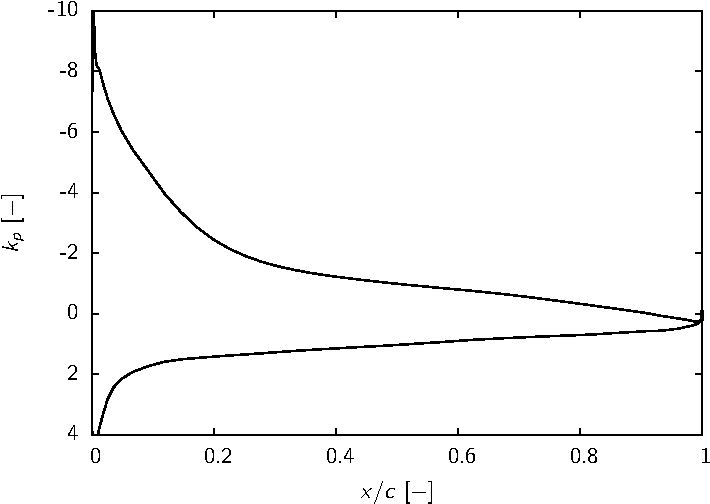
\includegraphics[width=0.28\textwidth]{DREAM_LS_KP_50_REAR_PPT.pdf}
   & 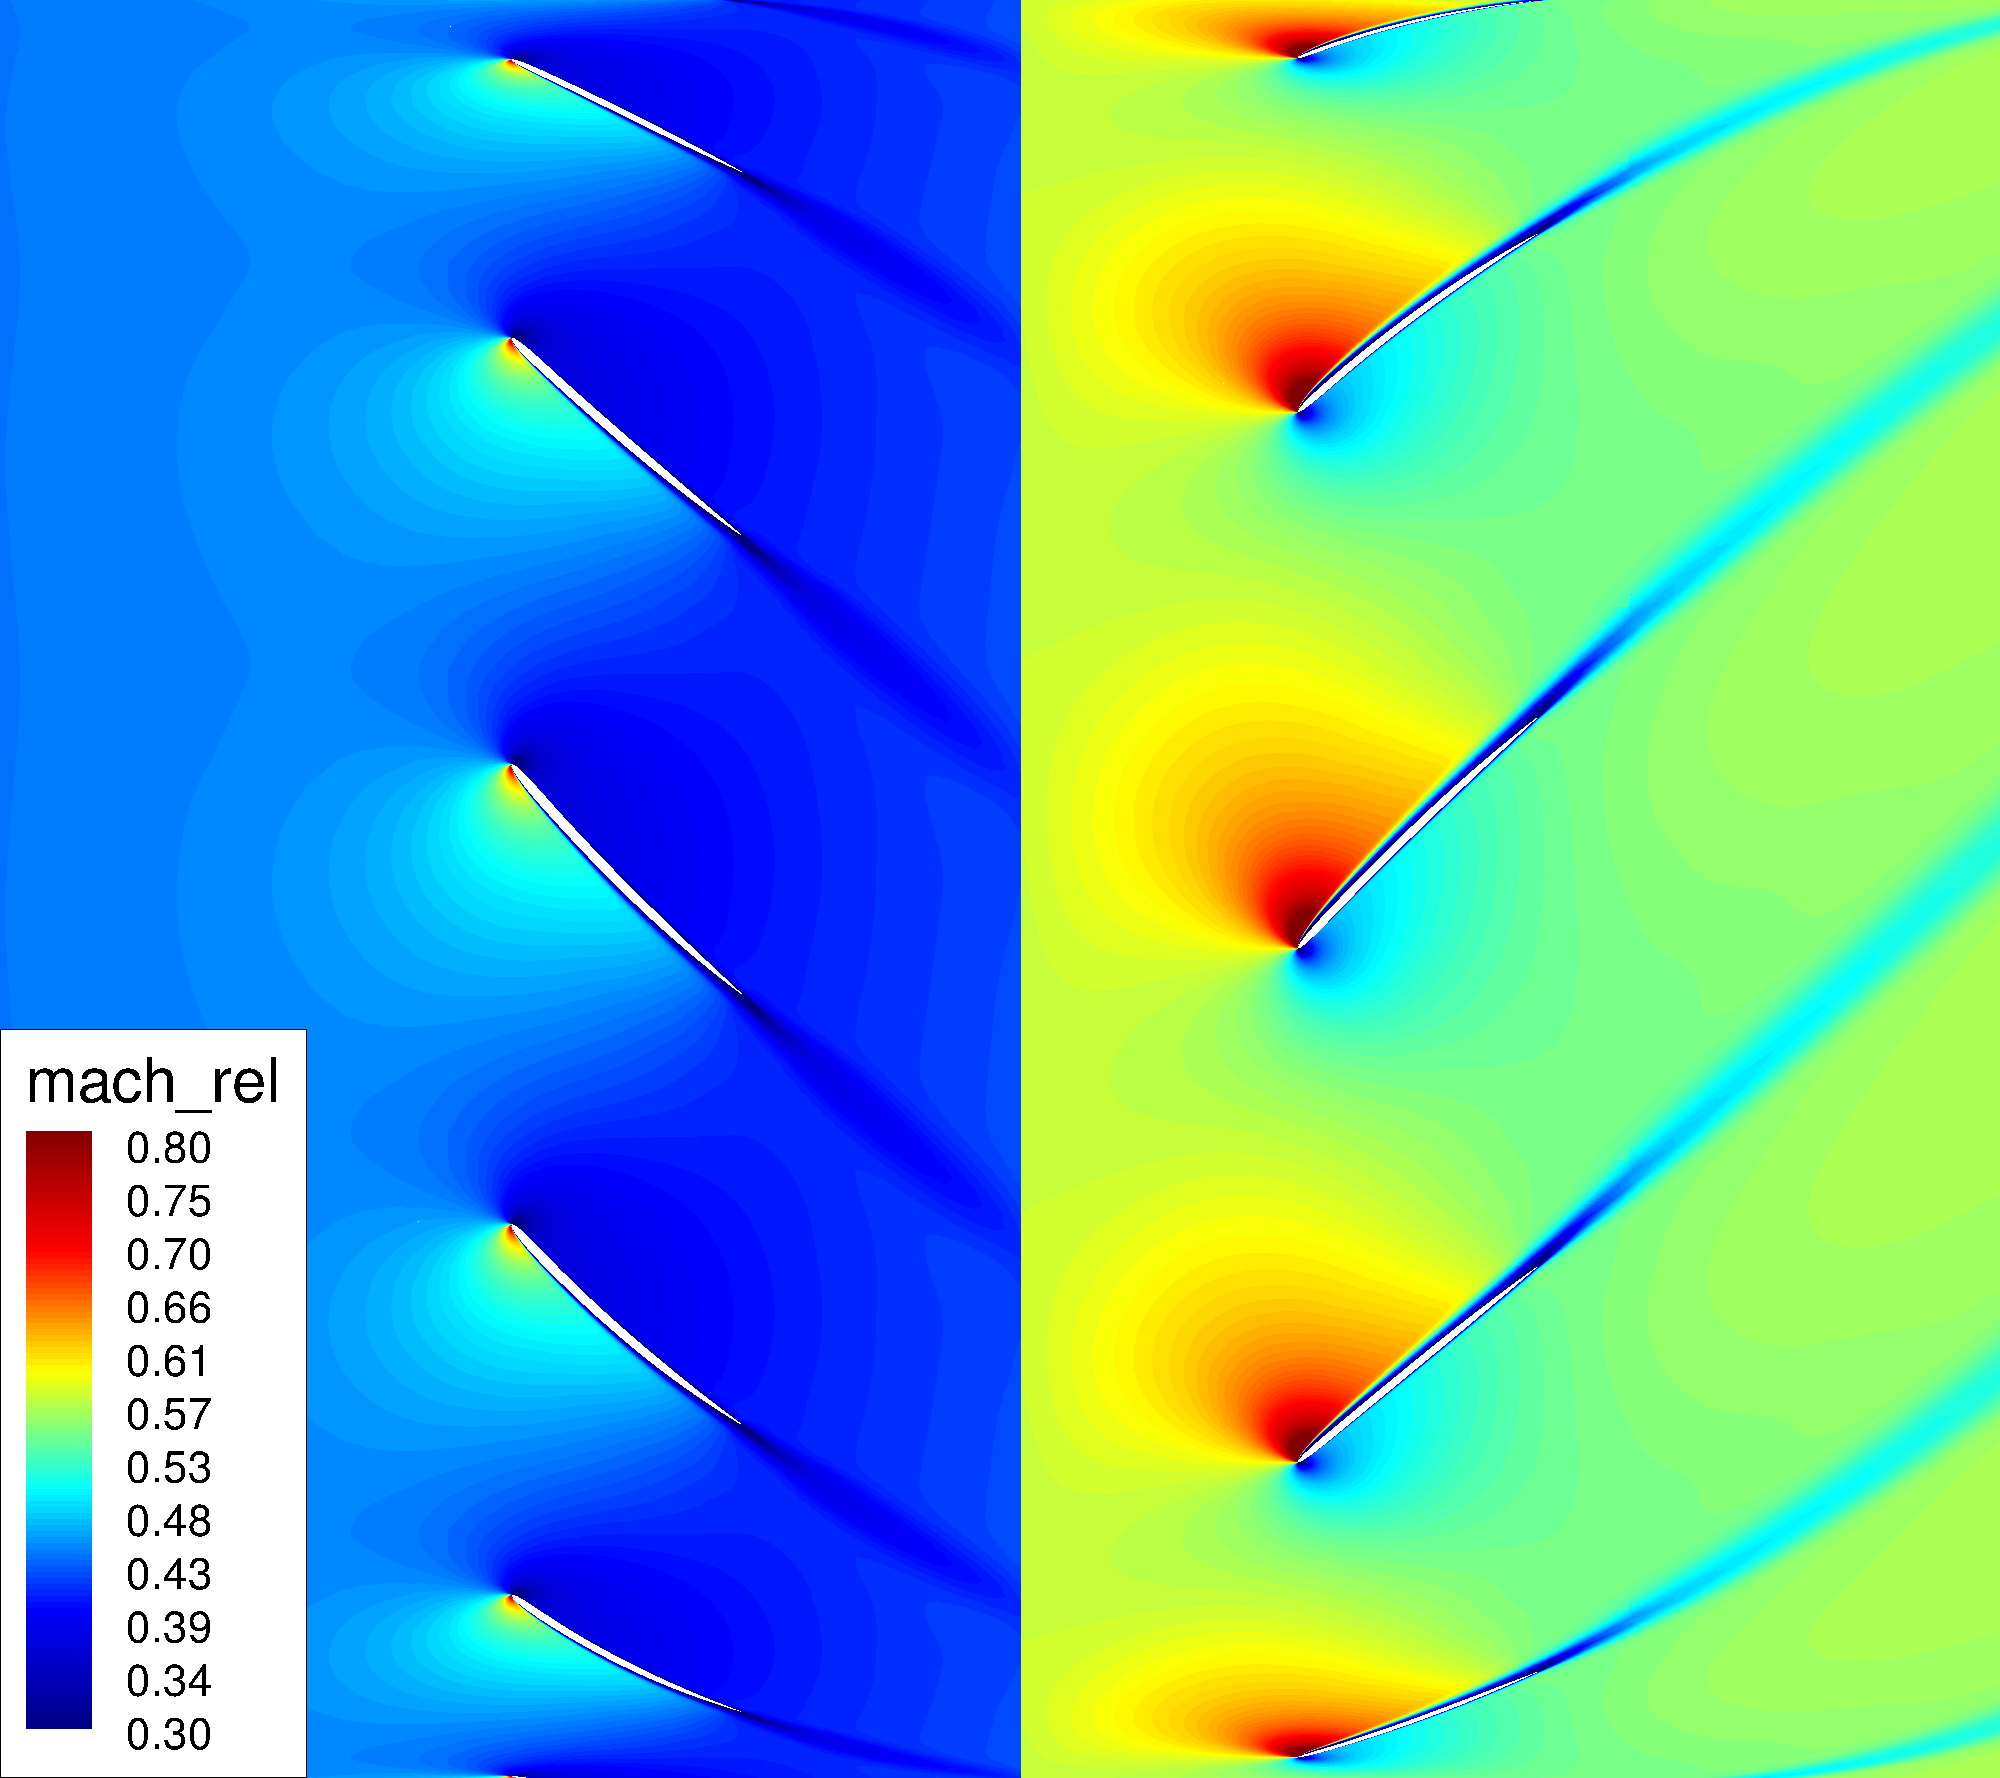
\includegraphics[width=0.28\textwidth]{DREAM_LS_RANS_roe2_sa_slice_r_50_mach_rel.png}\\
   \rotatebox{90}{\qquad\qquad 75~\%} 
   & 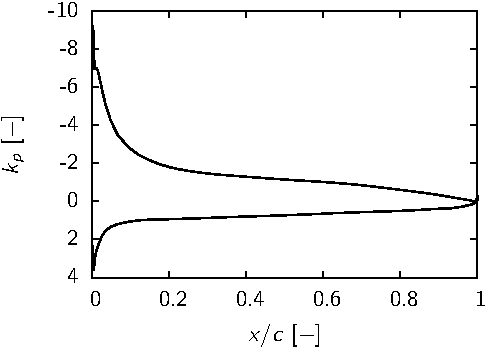
\includegraphics[width=0.28\textwidth]{DREAM_LS_KP_75_FRONT_PPT.pdf}
   & 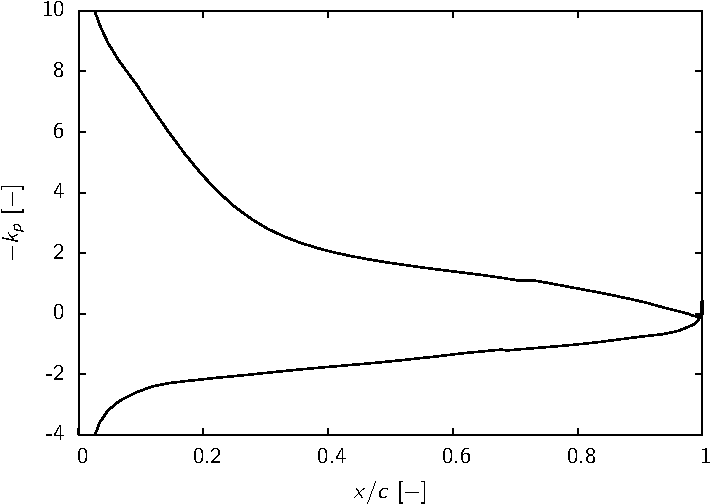
\includegraphics[width=0.28\textwidth]{DREAM_LS_KP_75_REAR_PPT.pdf}
   & 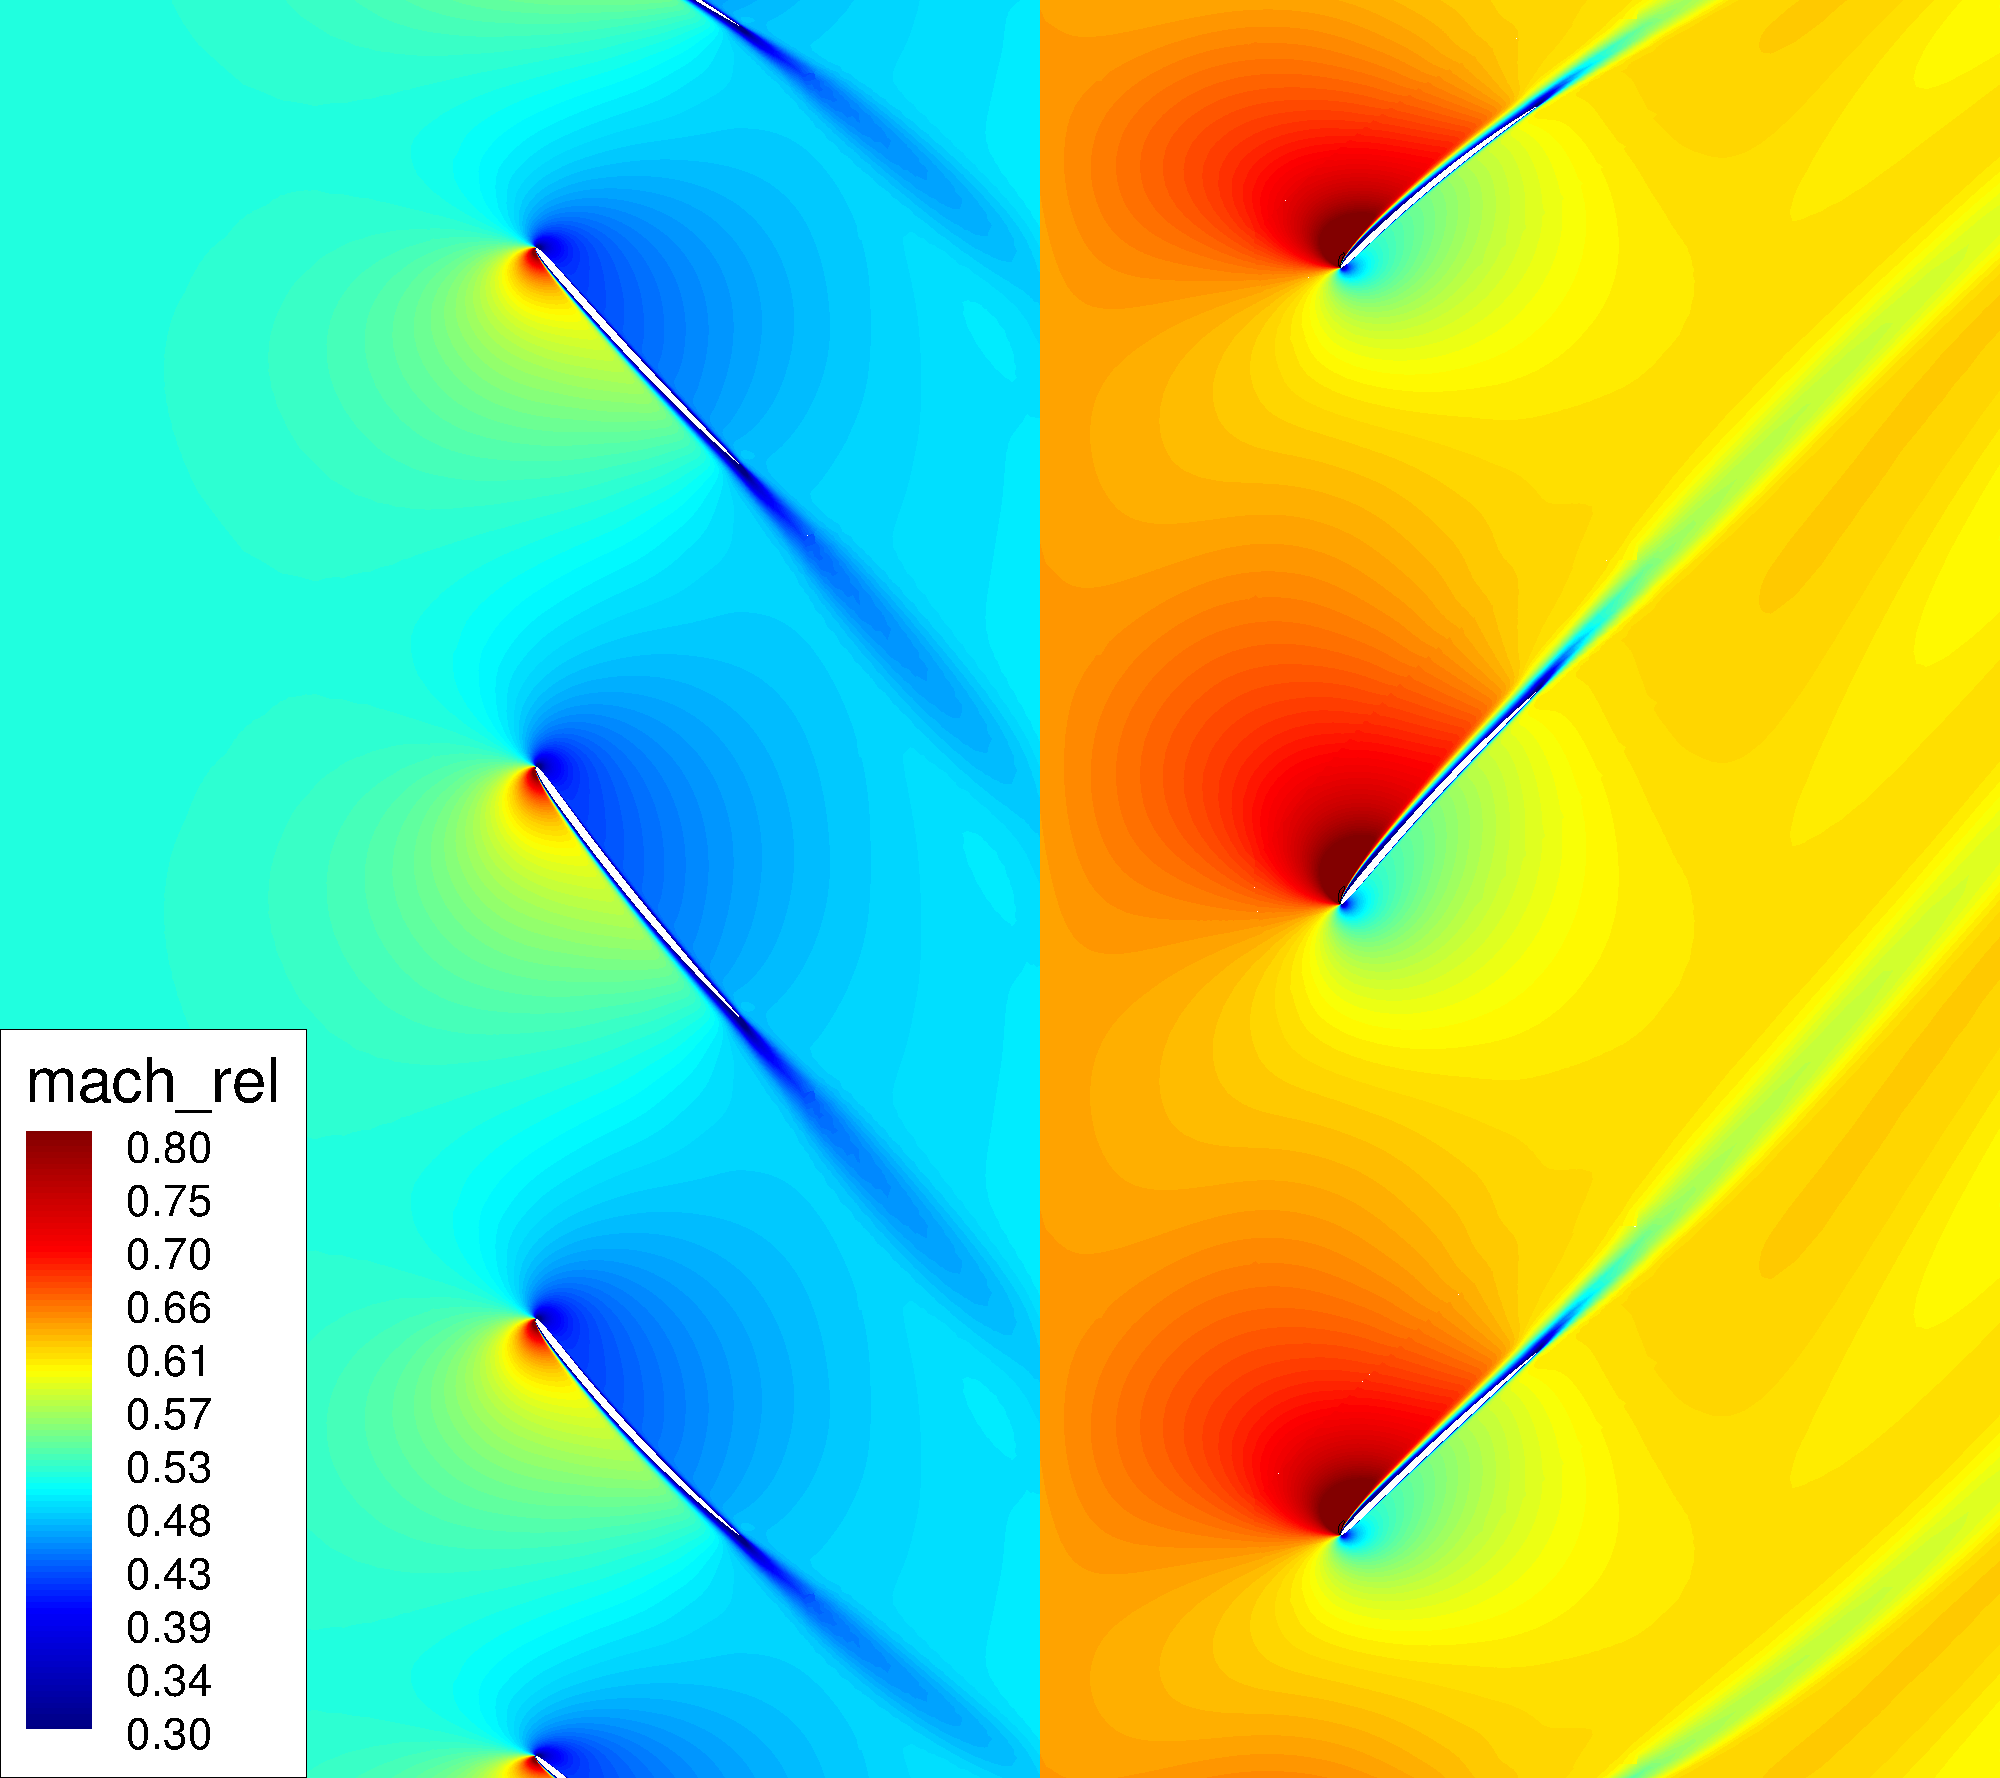
\includegraphics[width=0.28\textwidth]{DREAM_LS_RANS_roe2_sa_slice_r_75_mach_rel.png}\\
   \rotatebox{90}{\qquad\qquad 90~\%} 
   & 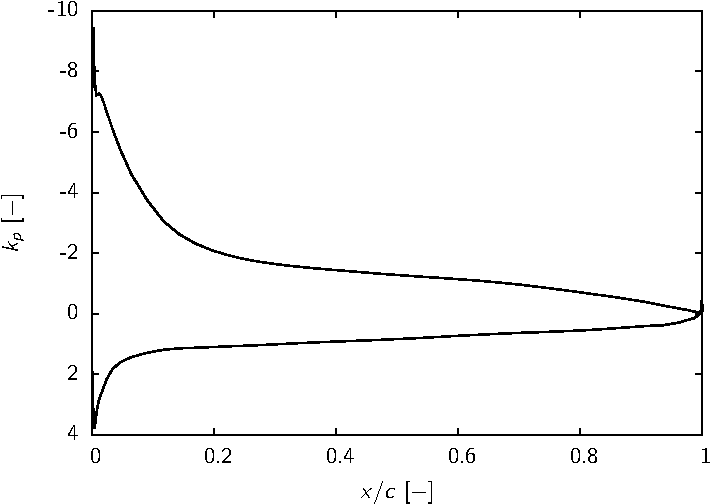
\includegraphics[width=0.28\textwidth]{DREAM_LS_KP_90_FRONT_PPT.pdf}
   & 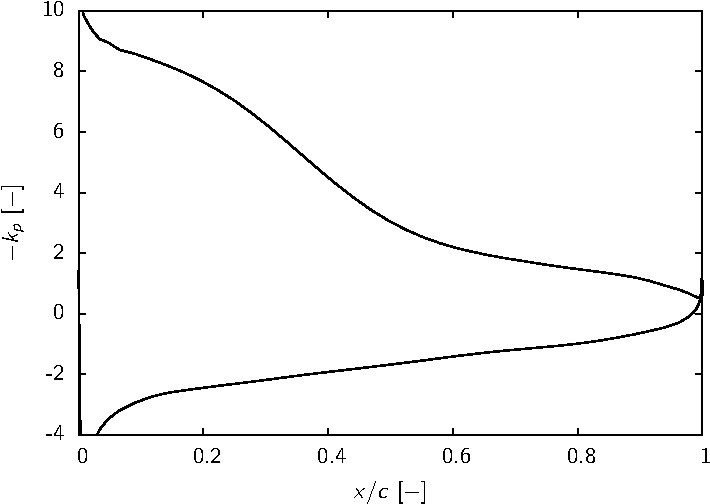
\includegraphics[width=0.28\textwidth]{DREAM_LS_KP_90_REAR_PPT.pdf}
   & 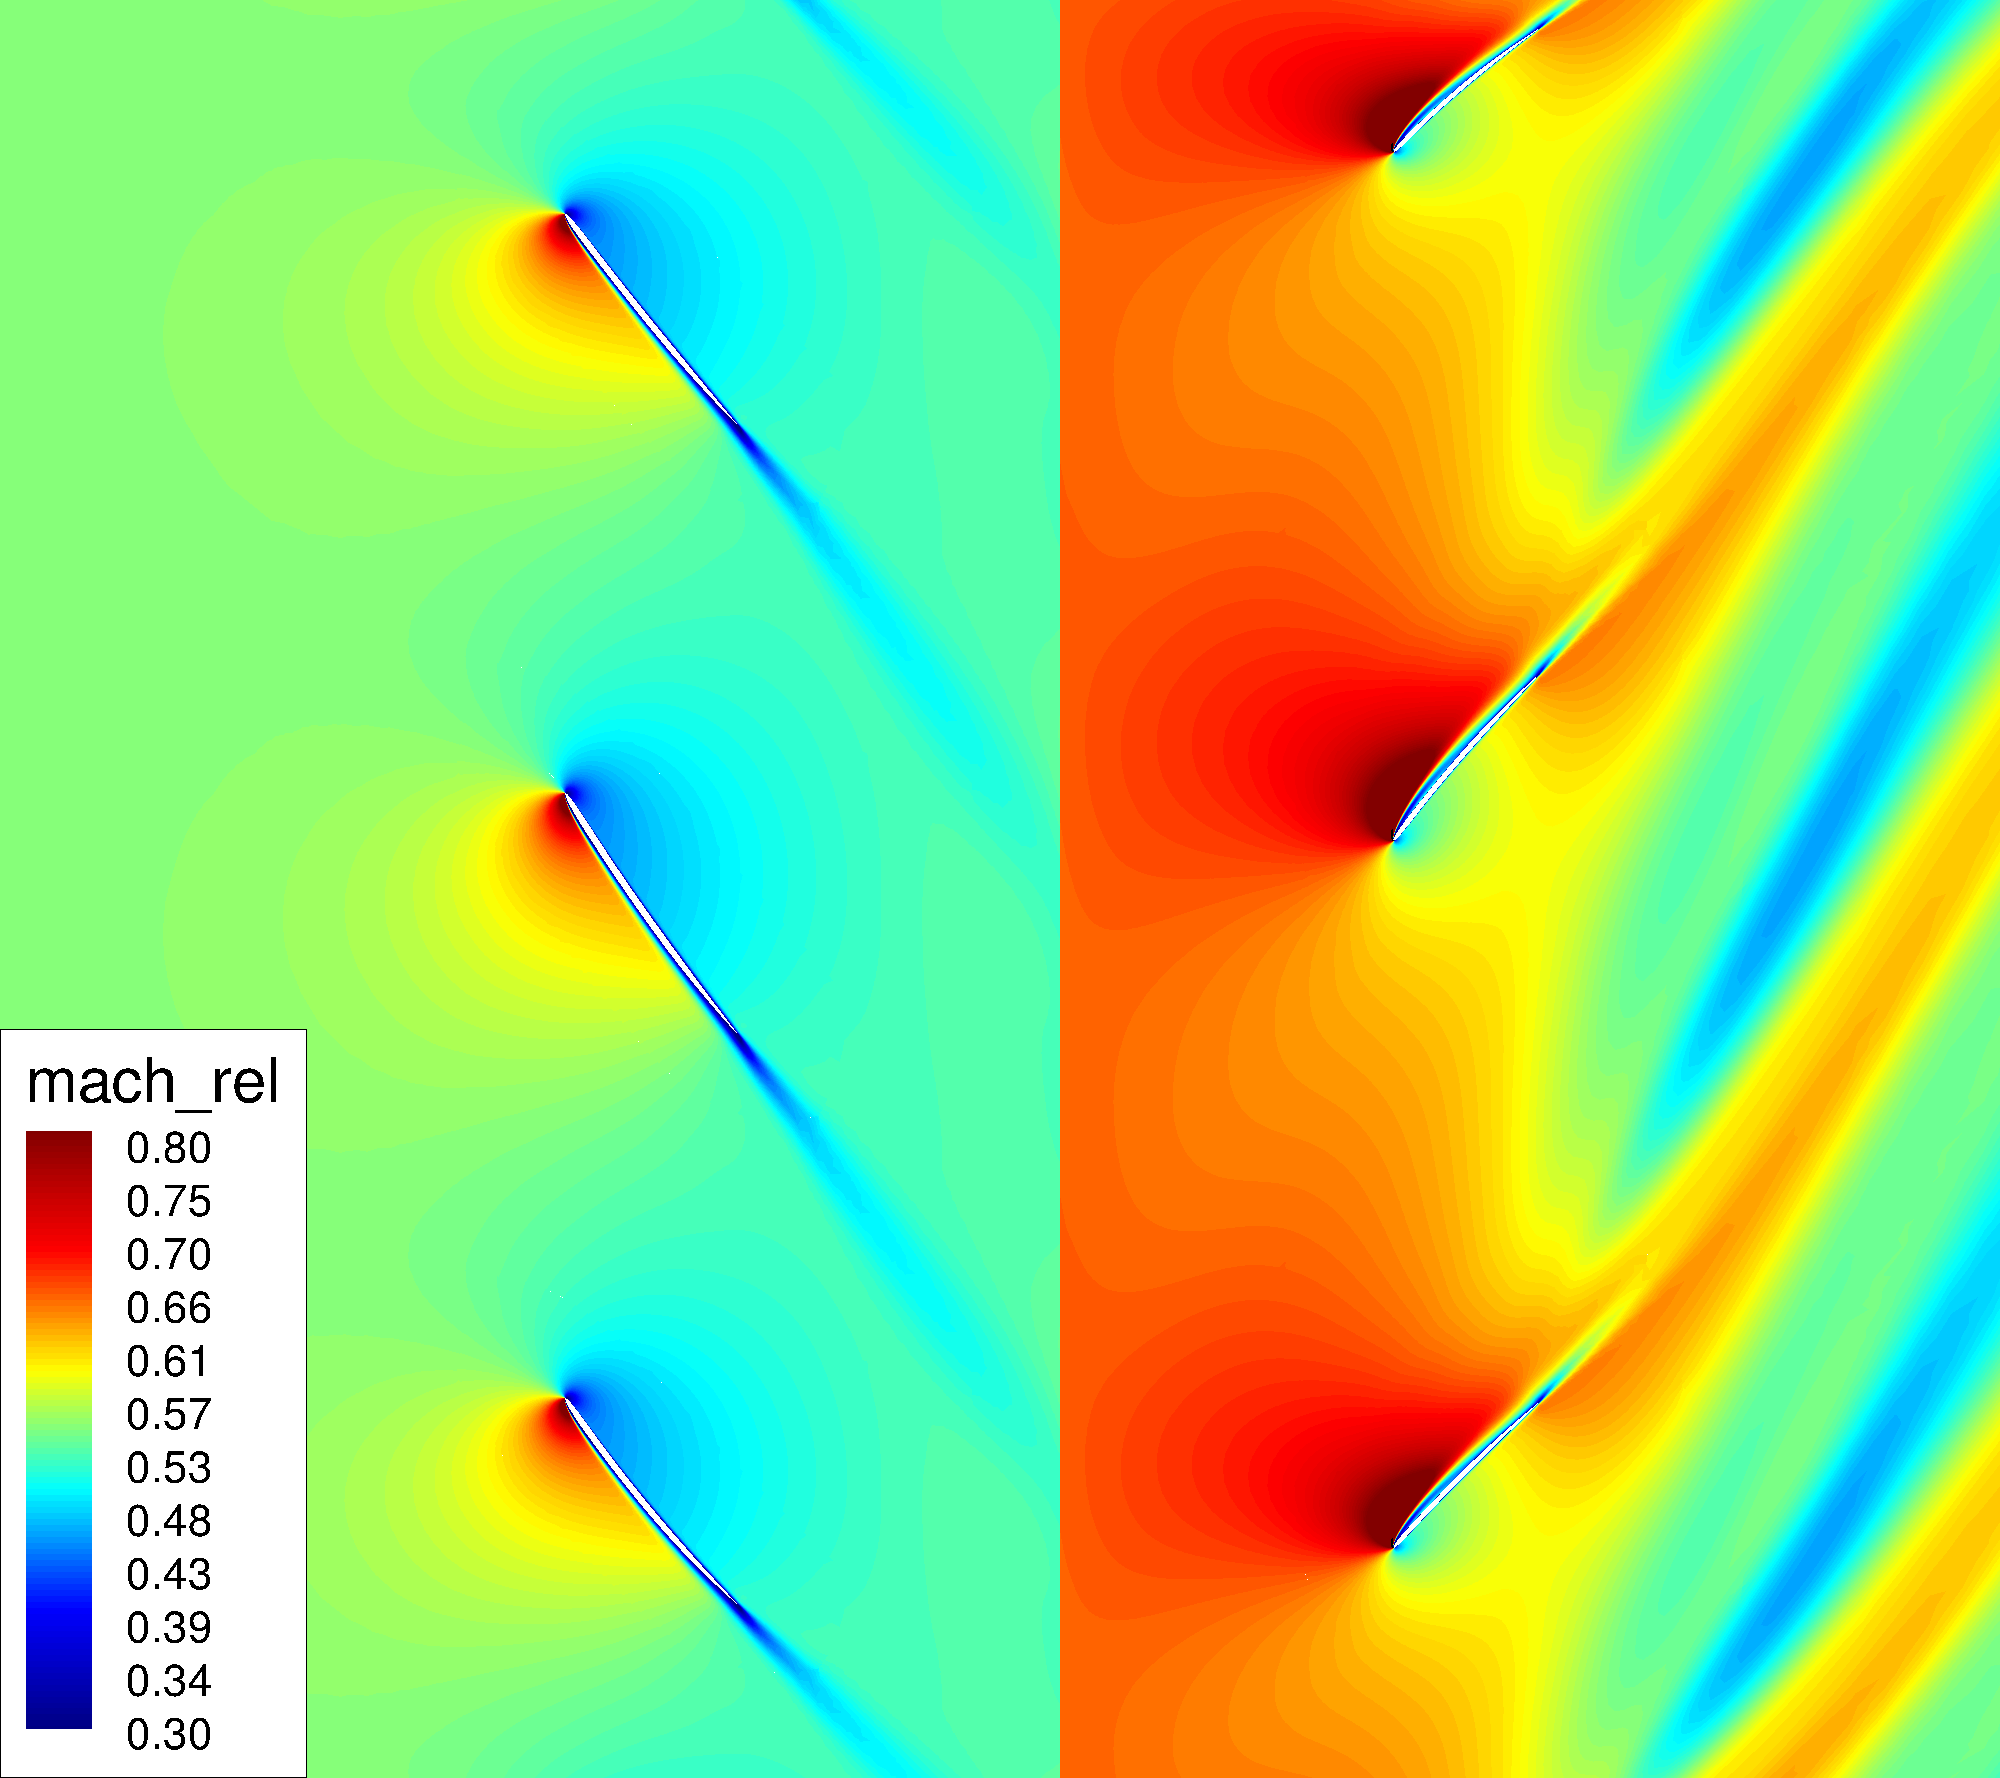
\includegraphics[width=0.28\textwidth]{DREAM_LS_RANS_roe2_sa_slice_r_90_mach_rel.png}\\
   \rotatebox{90}{\qquad\qquad 95~\%} 
   & 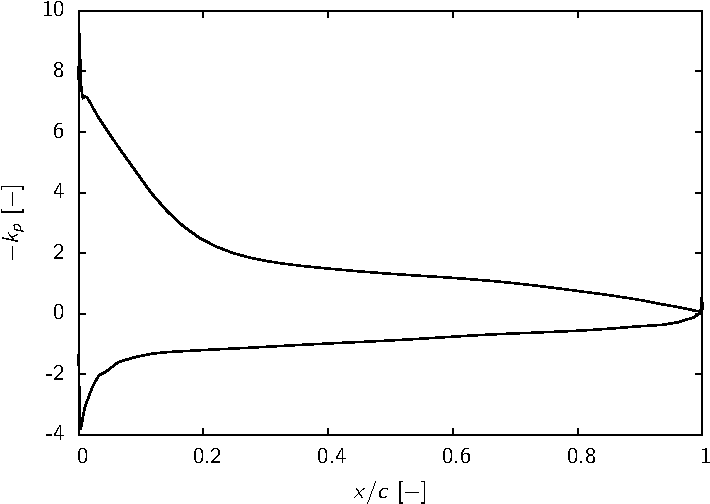
\includegraphics[width=0.28\textwidth]{DREAM_LS_KP_95_FRONT_PPT.pdf}
   & 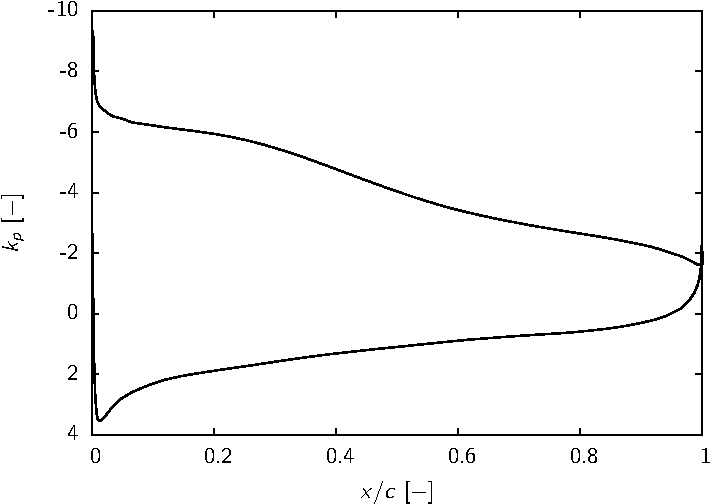
\includegraphics[width=0.28\textwidth]{DREAM_LS_KP_95_REAR_PPT.pdf}
   & 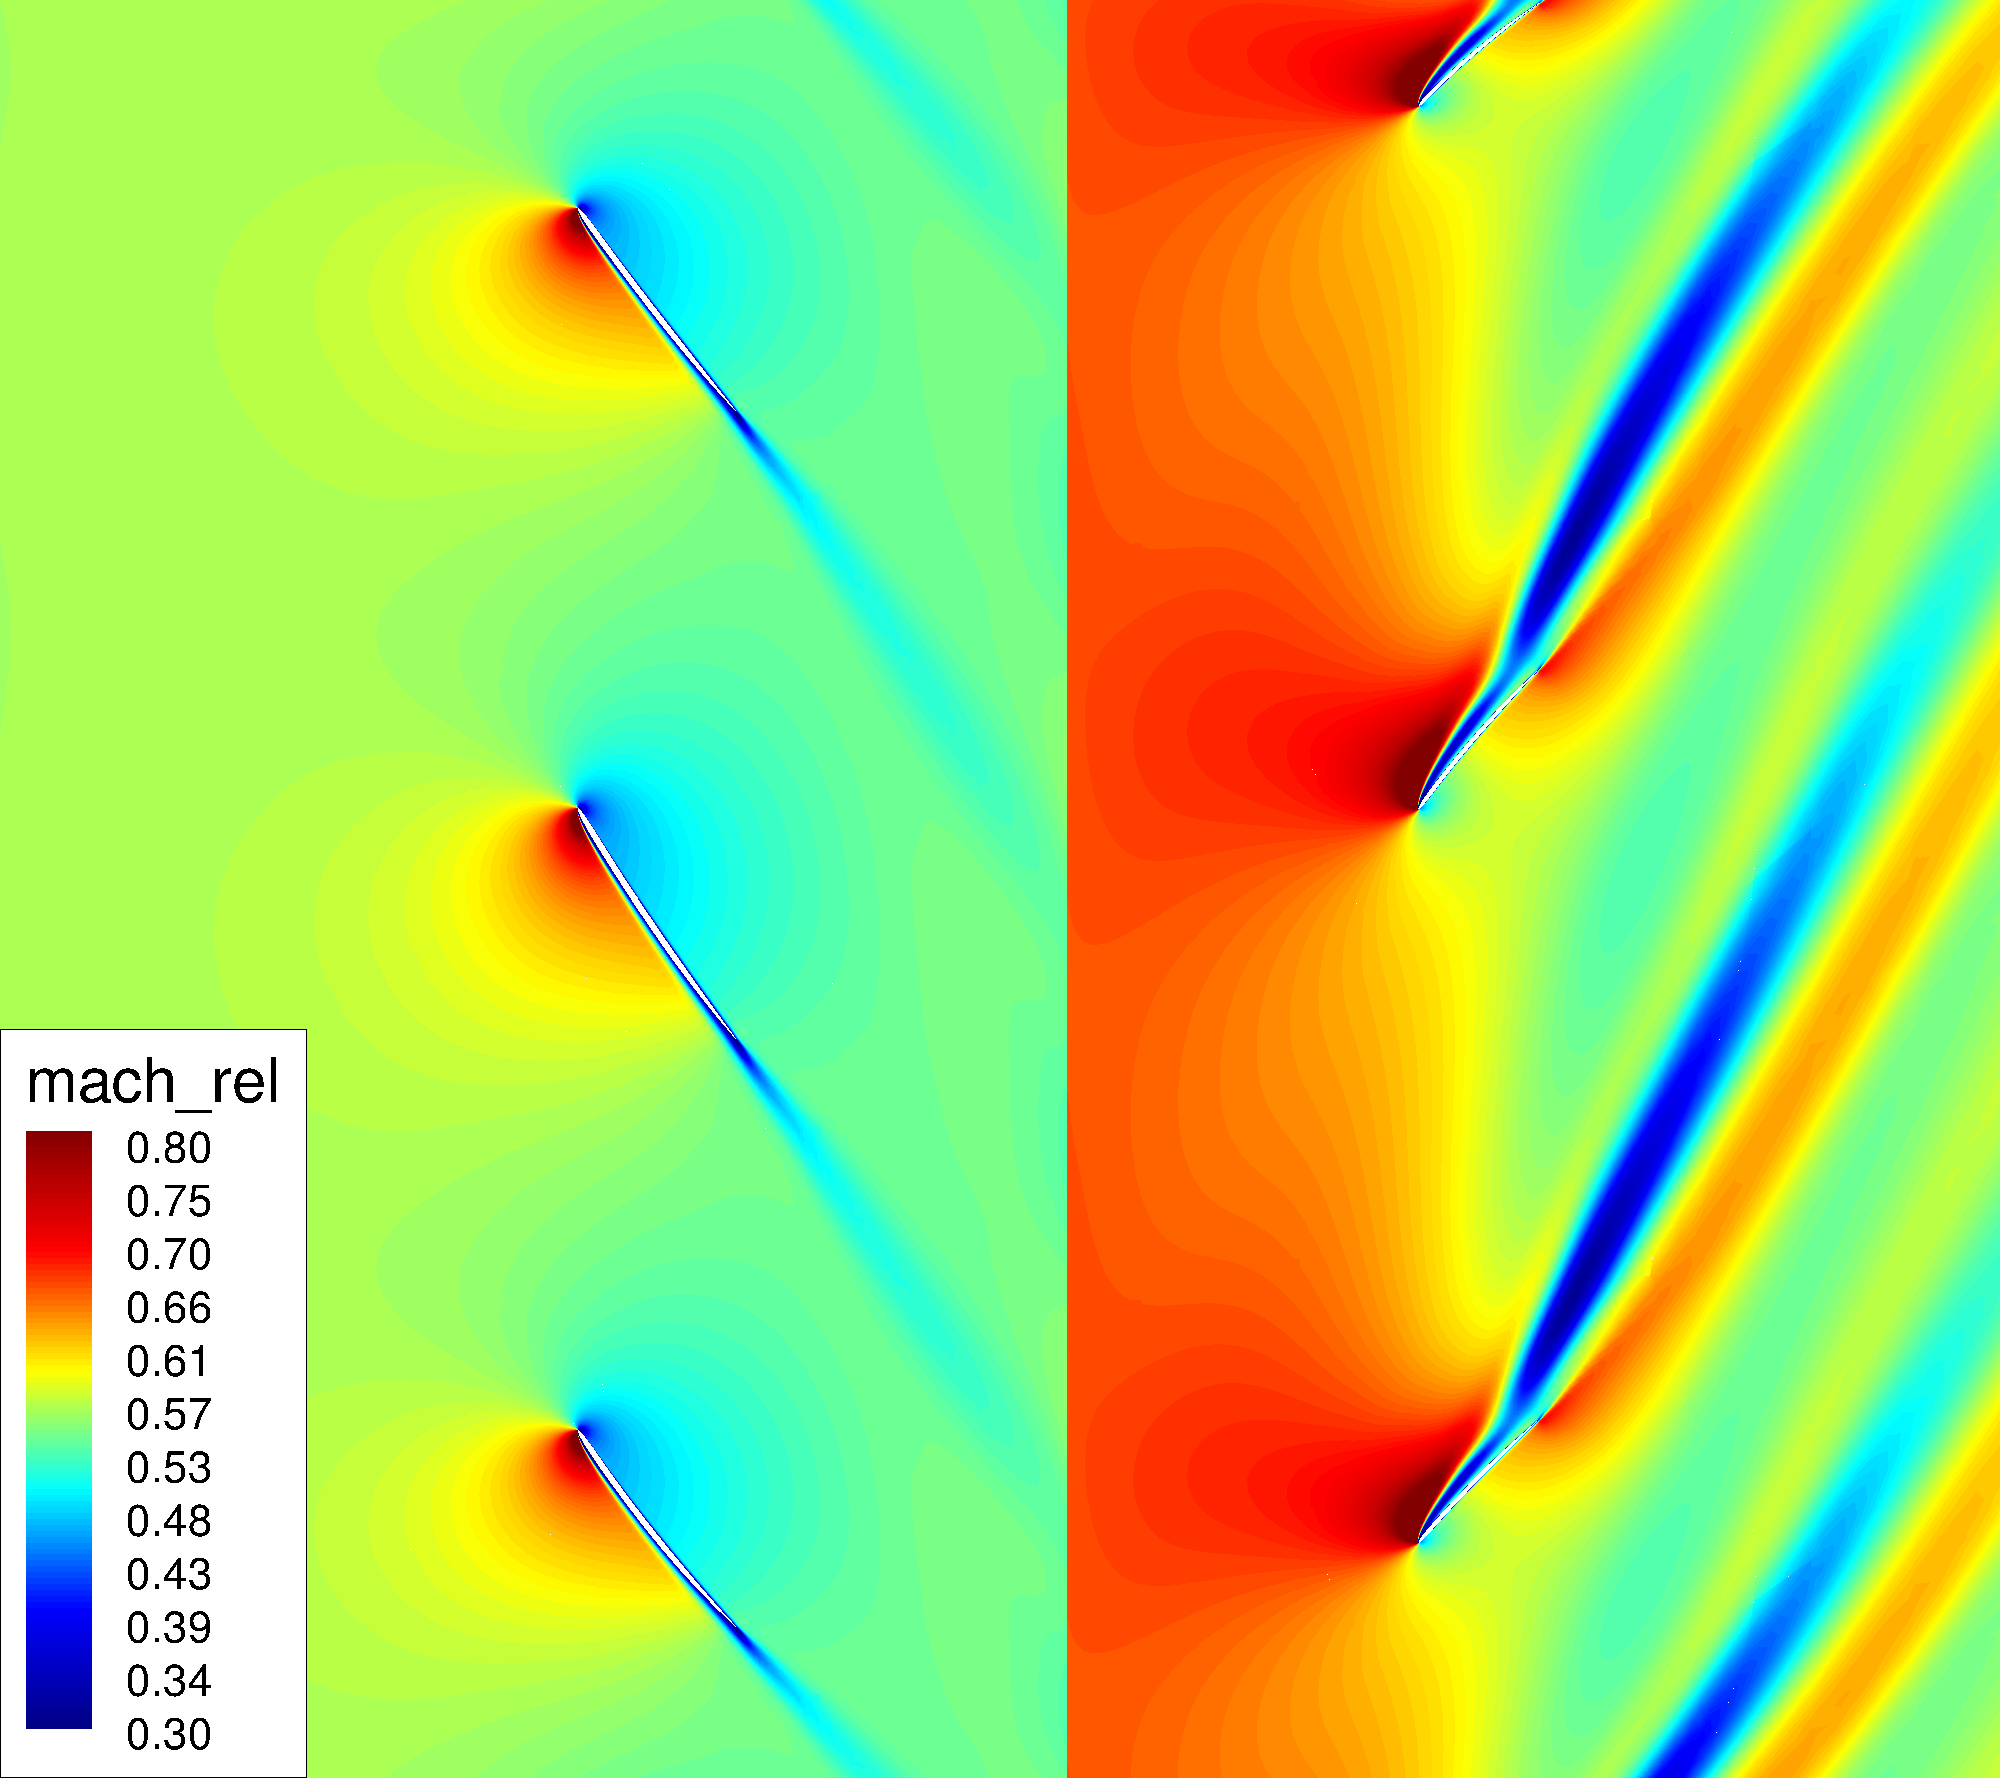
\includegraphics[width=0.28\textwidth]{DREAM_LS_RANS_roe2_sa_slice_r_95_mach_rel.png}  
 \end{tabular}
 \caption{Low-speed isolated configuration: pressure coefficient and relative Mach
 number contours at different radial position.}
 \label{fig:dream_ls_mach_kp}
\end{figure}

Axial cuts of the entropy are shown in Figure~\ref{fig:dream_ls_steady_entropy}.
The axial positions are the four planes $P3$, $P4$, $P5$
and $P6$ as defined in Figure~\ref{fig:dream_ls_position_radial}.
The tip vortices generated by the front rotor are seen in the $P3$
axial plane. The mixing plane approach is used for the steady computations
presented here. This is emphasized by the $P4$ axial cut of entropy. A
smooth, spatially-averaged field of entropy is seen with a 
ring of losses attributed to the front rotor tip vortices. This is of course the main
weakness of the steady approach used here to compute the CROR configuration.
In fact, as recalled in Chap.~\ref{cha:cror}, the tip vortices and the wakes shed by the
front rotor blades can impact the rear rotor blades and thus generate
exceeding level of unsteadinesses, responsible for noise and vibration. As the influence
of the front rotor tip vortices is azimuthally-averaged, it is
lessened. Therefore unsteady computations will be needed to
predict the unsteady interactions of the front rotor with the rear one.
This is the aim of the forthcoming Section~\ref{sec:dream_ls_rigid_results}.
The remaining axial planes extracted at $P5$ and $P6$ depict the strong loading
of the rear rotor blades. In fact, baring in mind that the
axial planes are equidistant from the blades, the larger the loss traces,
the stronger the loading of the blades. 
According to the Euler theorem applied on the two
rotors, the enthalpy variation is equal to the variation of 
the dot product of the rotational 
velocity $U=\Omega R$ to the tangential absolute velocity
$V_\theta$. If the inflow is similar on both rotors,
the work exchange should be the same. However,
the flow has been accelerated by the front rotor
resulting in a higher work exchange to obtain
the same deviation on the rear rotor.
This higher work exchange implies 
a greater loading of the rear rotor blades and thus
higher pressure gradients. Therefore,
the flow field will be more prone to boundary layer
separation, which is observed in practice in 
Fig.~\ref{fig:dream_ls_steady_entropy} by larger entropy
downstream the rear rotor blades.
Moreover, even though the
tip vortices shed by the front rotor 
blades are azimuthally-averaged,
their trace is still seen and seems to indicate that they will
interact with the rear rotor tip vortices.
\begin{figure}[htp]
  \centering
  \subfigure[$P3$]{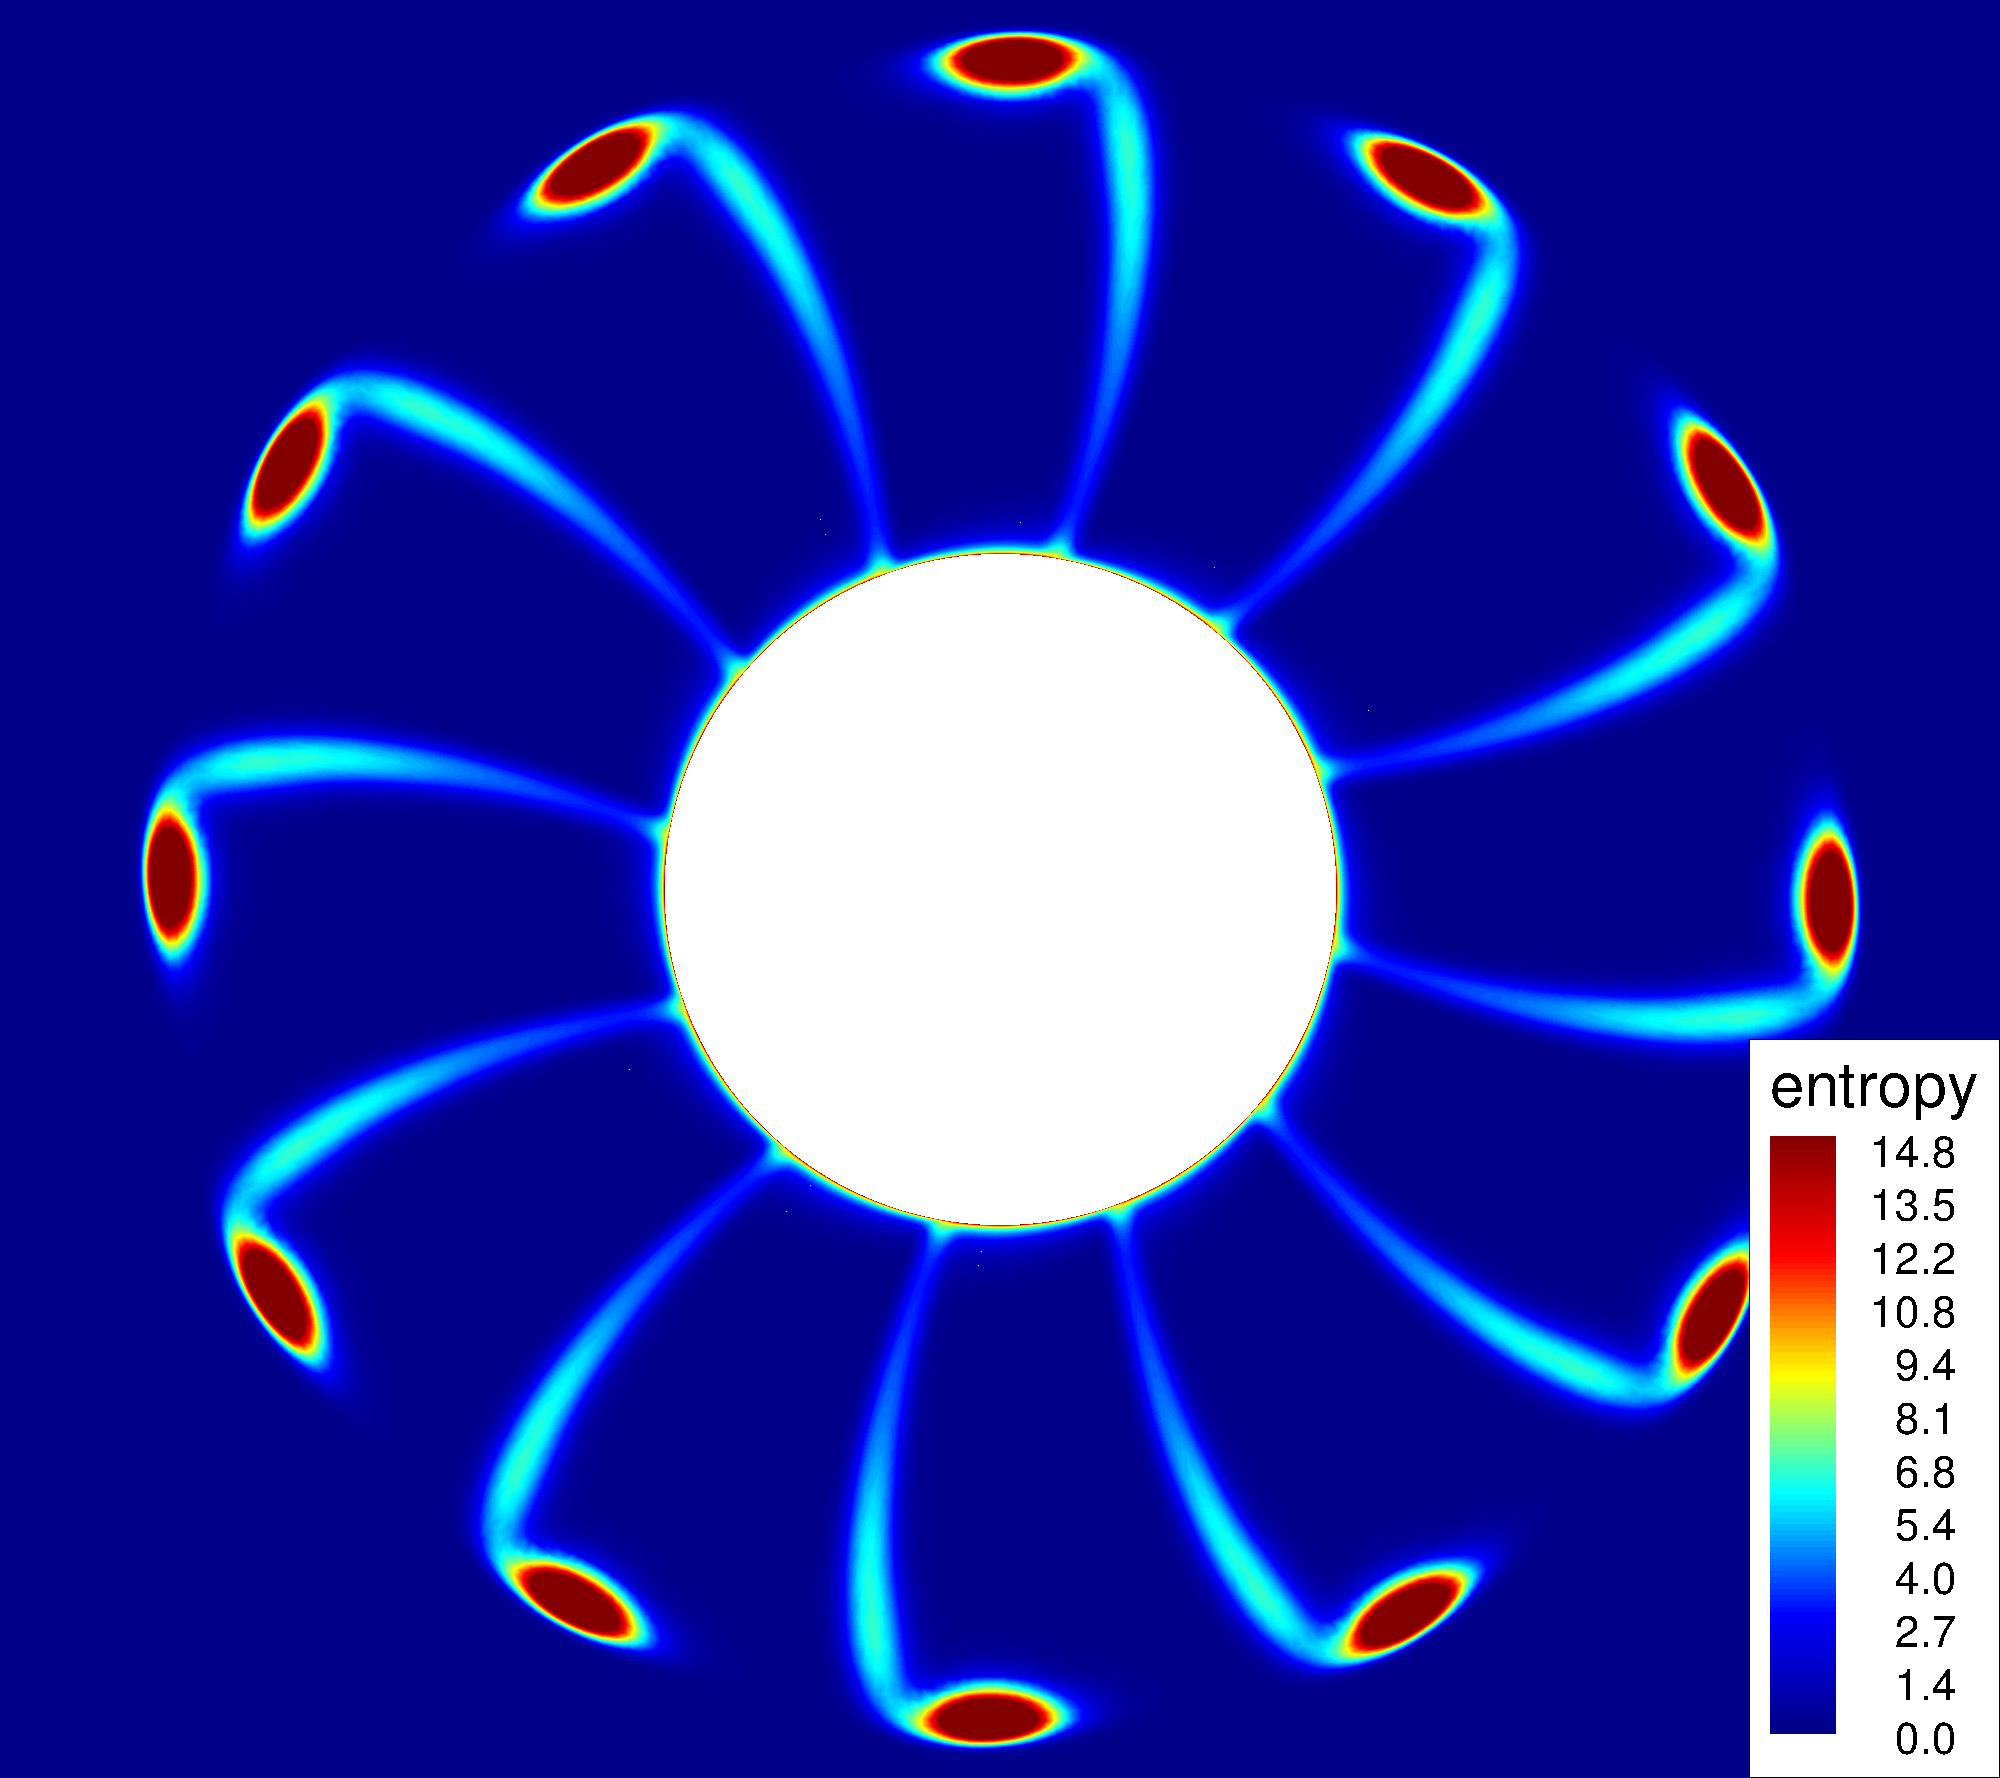
\includegraphics[width=.35\textwidth]{DREAM_LS_RANS_roe2_sa_slice_x_front_1_entropy.png}}
  \subfigure[$P4$]{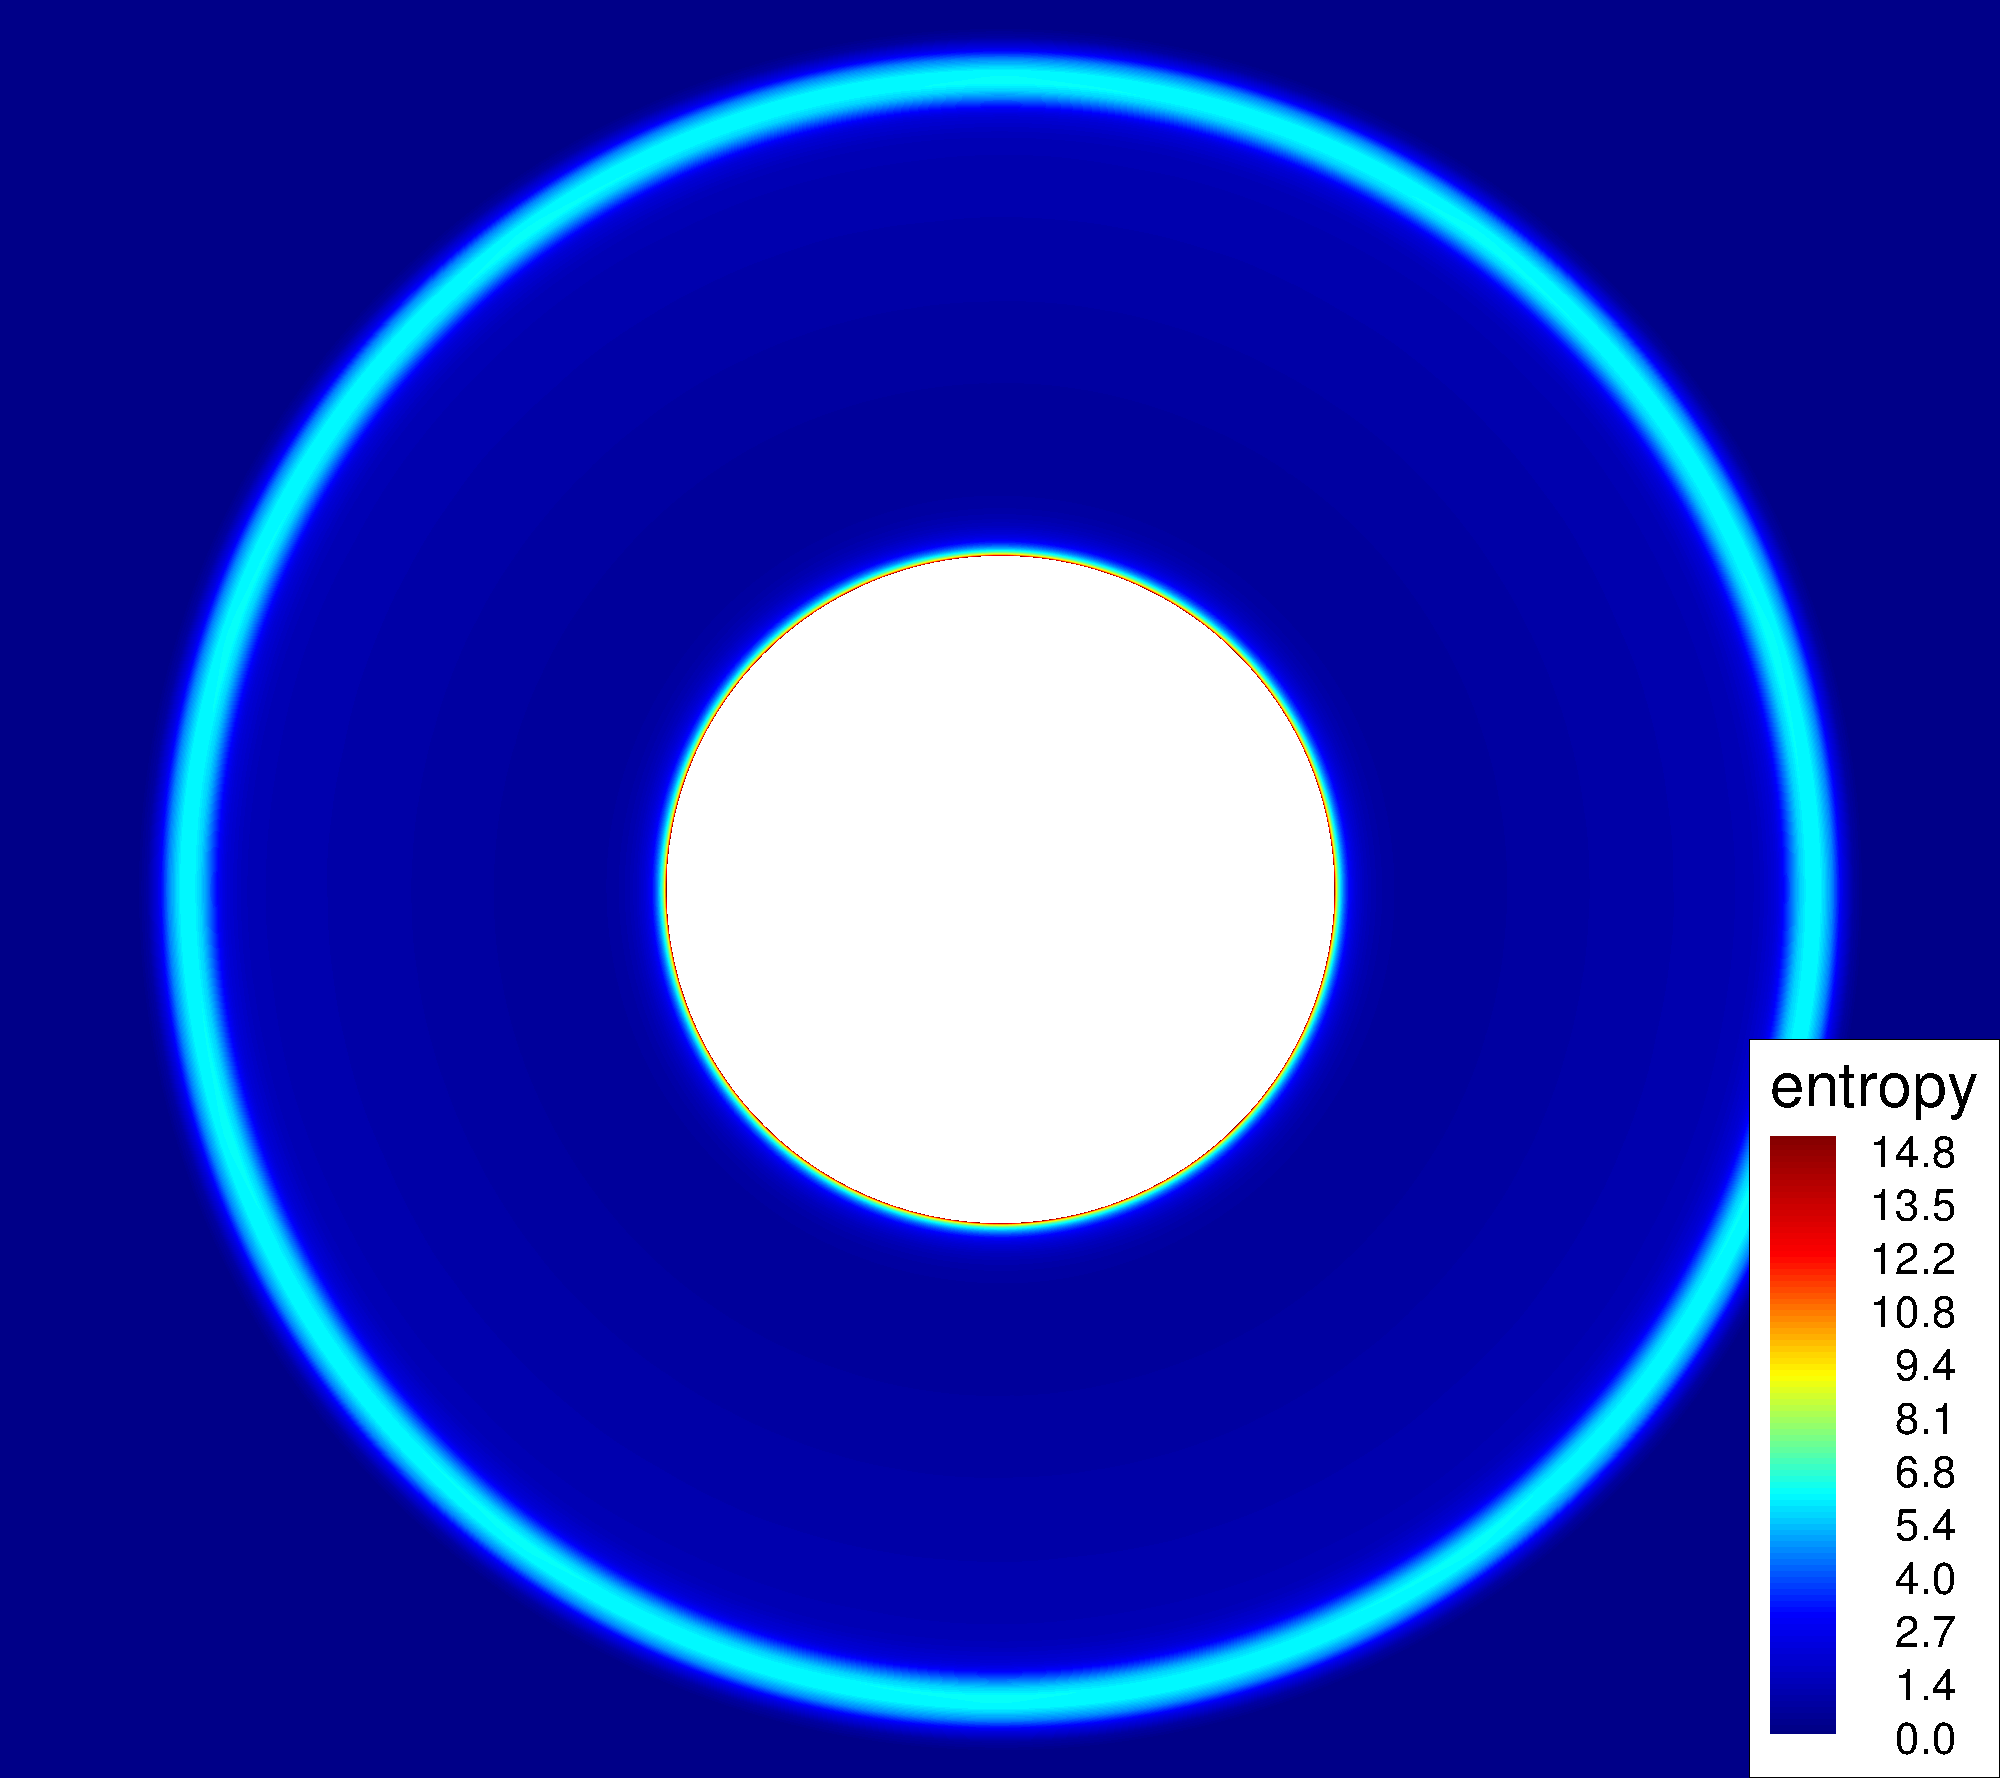
\includegraphics[width=.35\textwidth]{DREAM_LS_RANS_roe2_sa_slice_x_rear_-1_entropy.png}}
  \subfigure[$P5$]{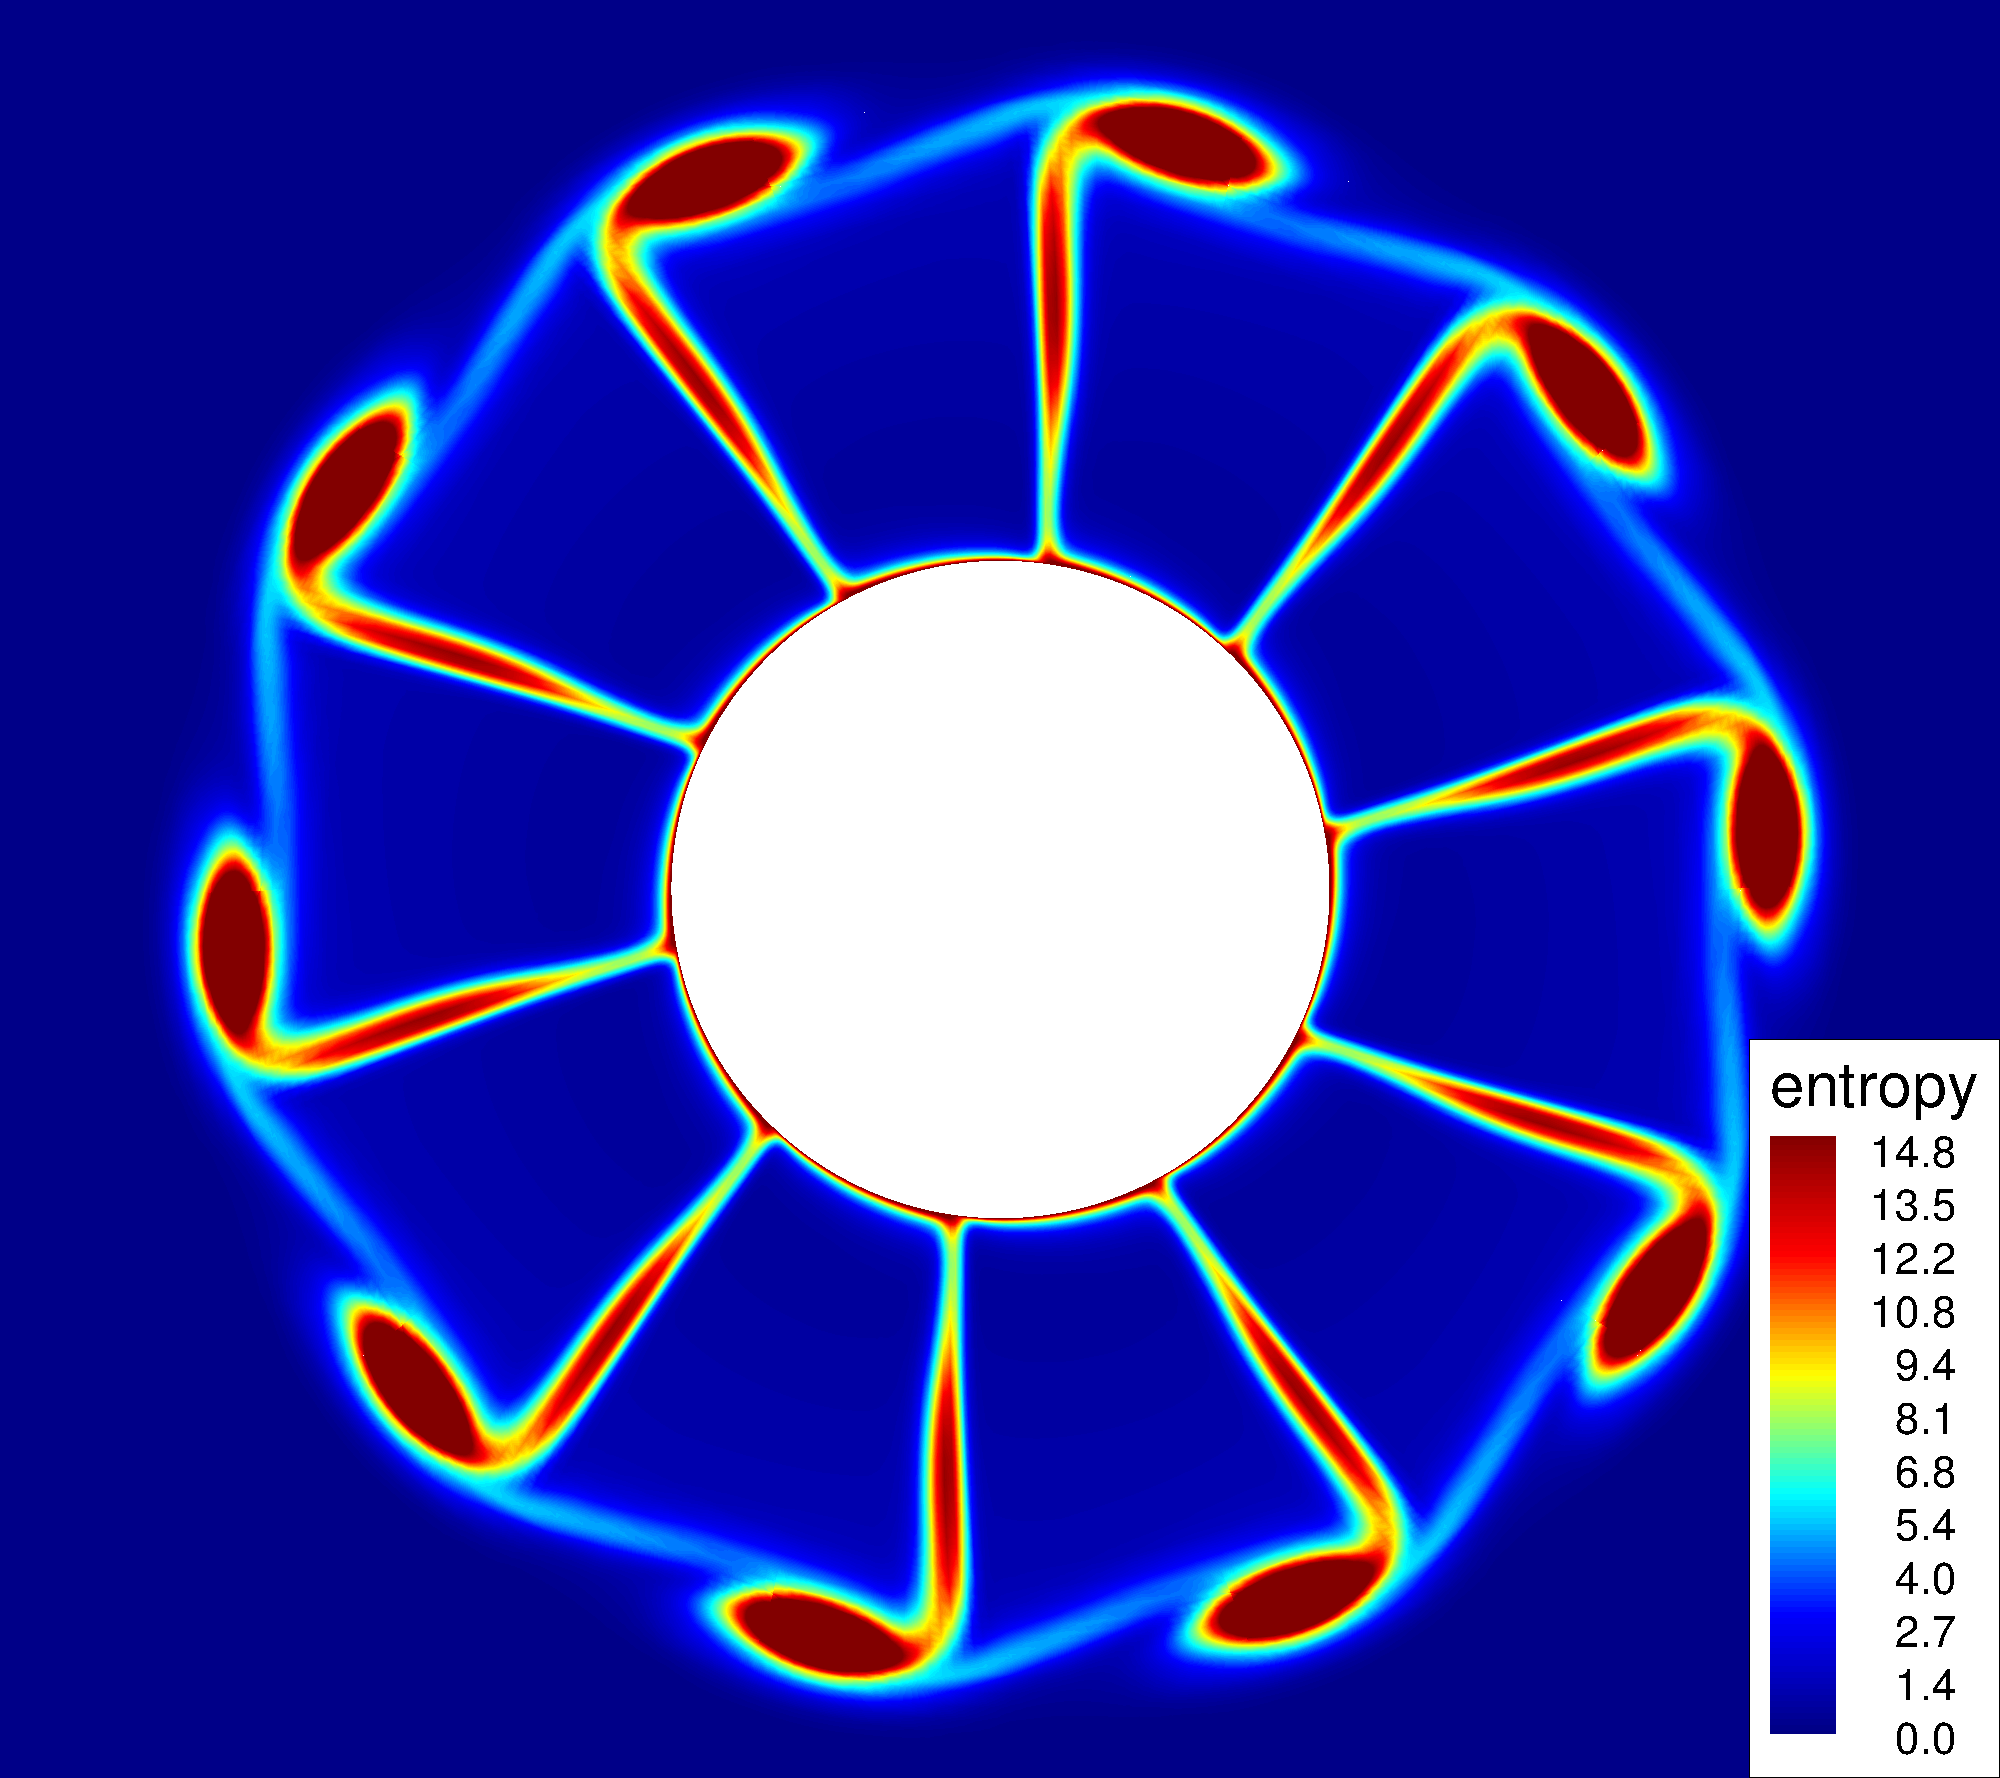
\includegraphics[width=.35\textwidth]{DREAM_LS_RANS_roe2_sa_slice_x_rear_1_entropy.png}}
  \subfigure[$P6$]{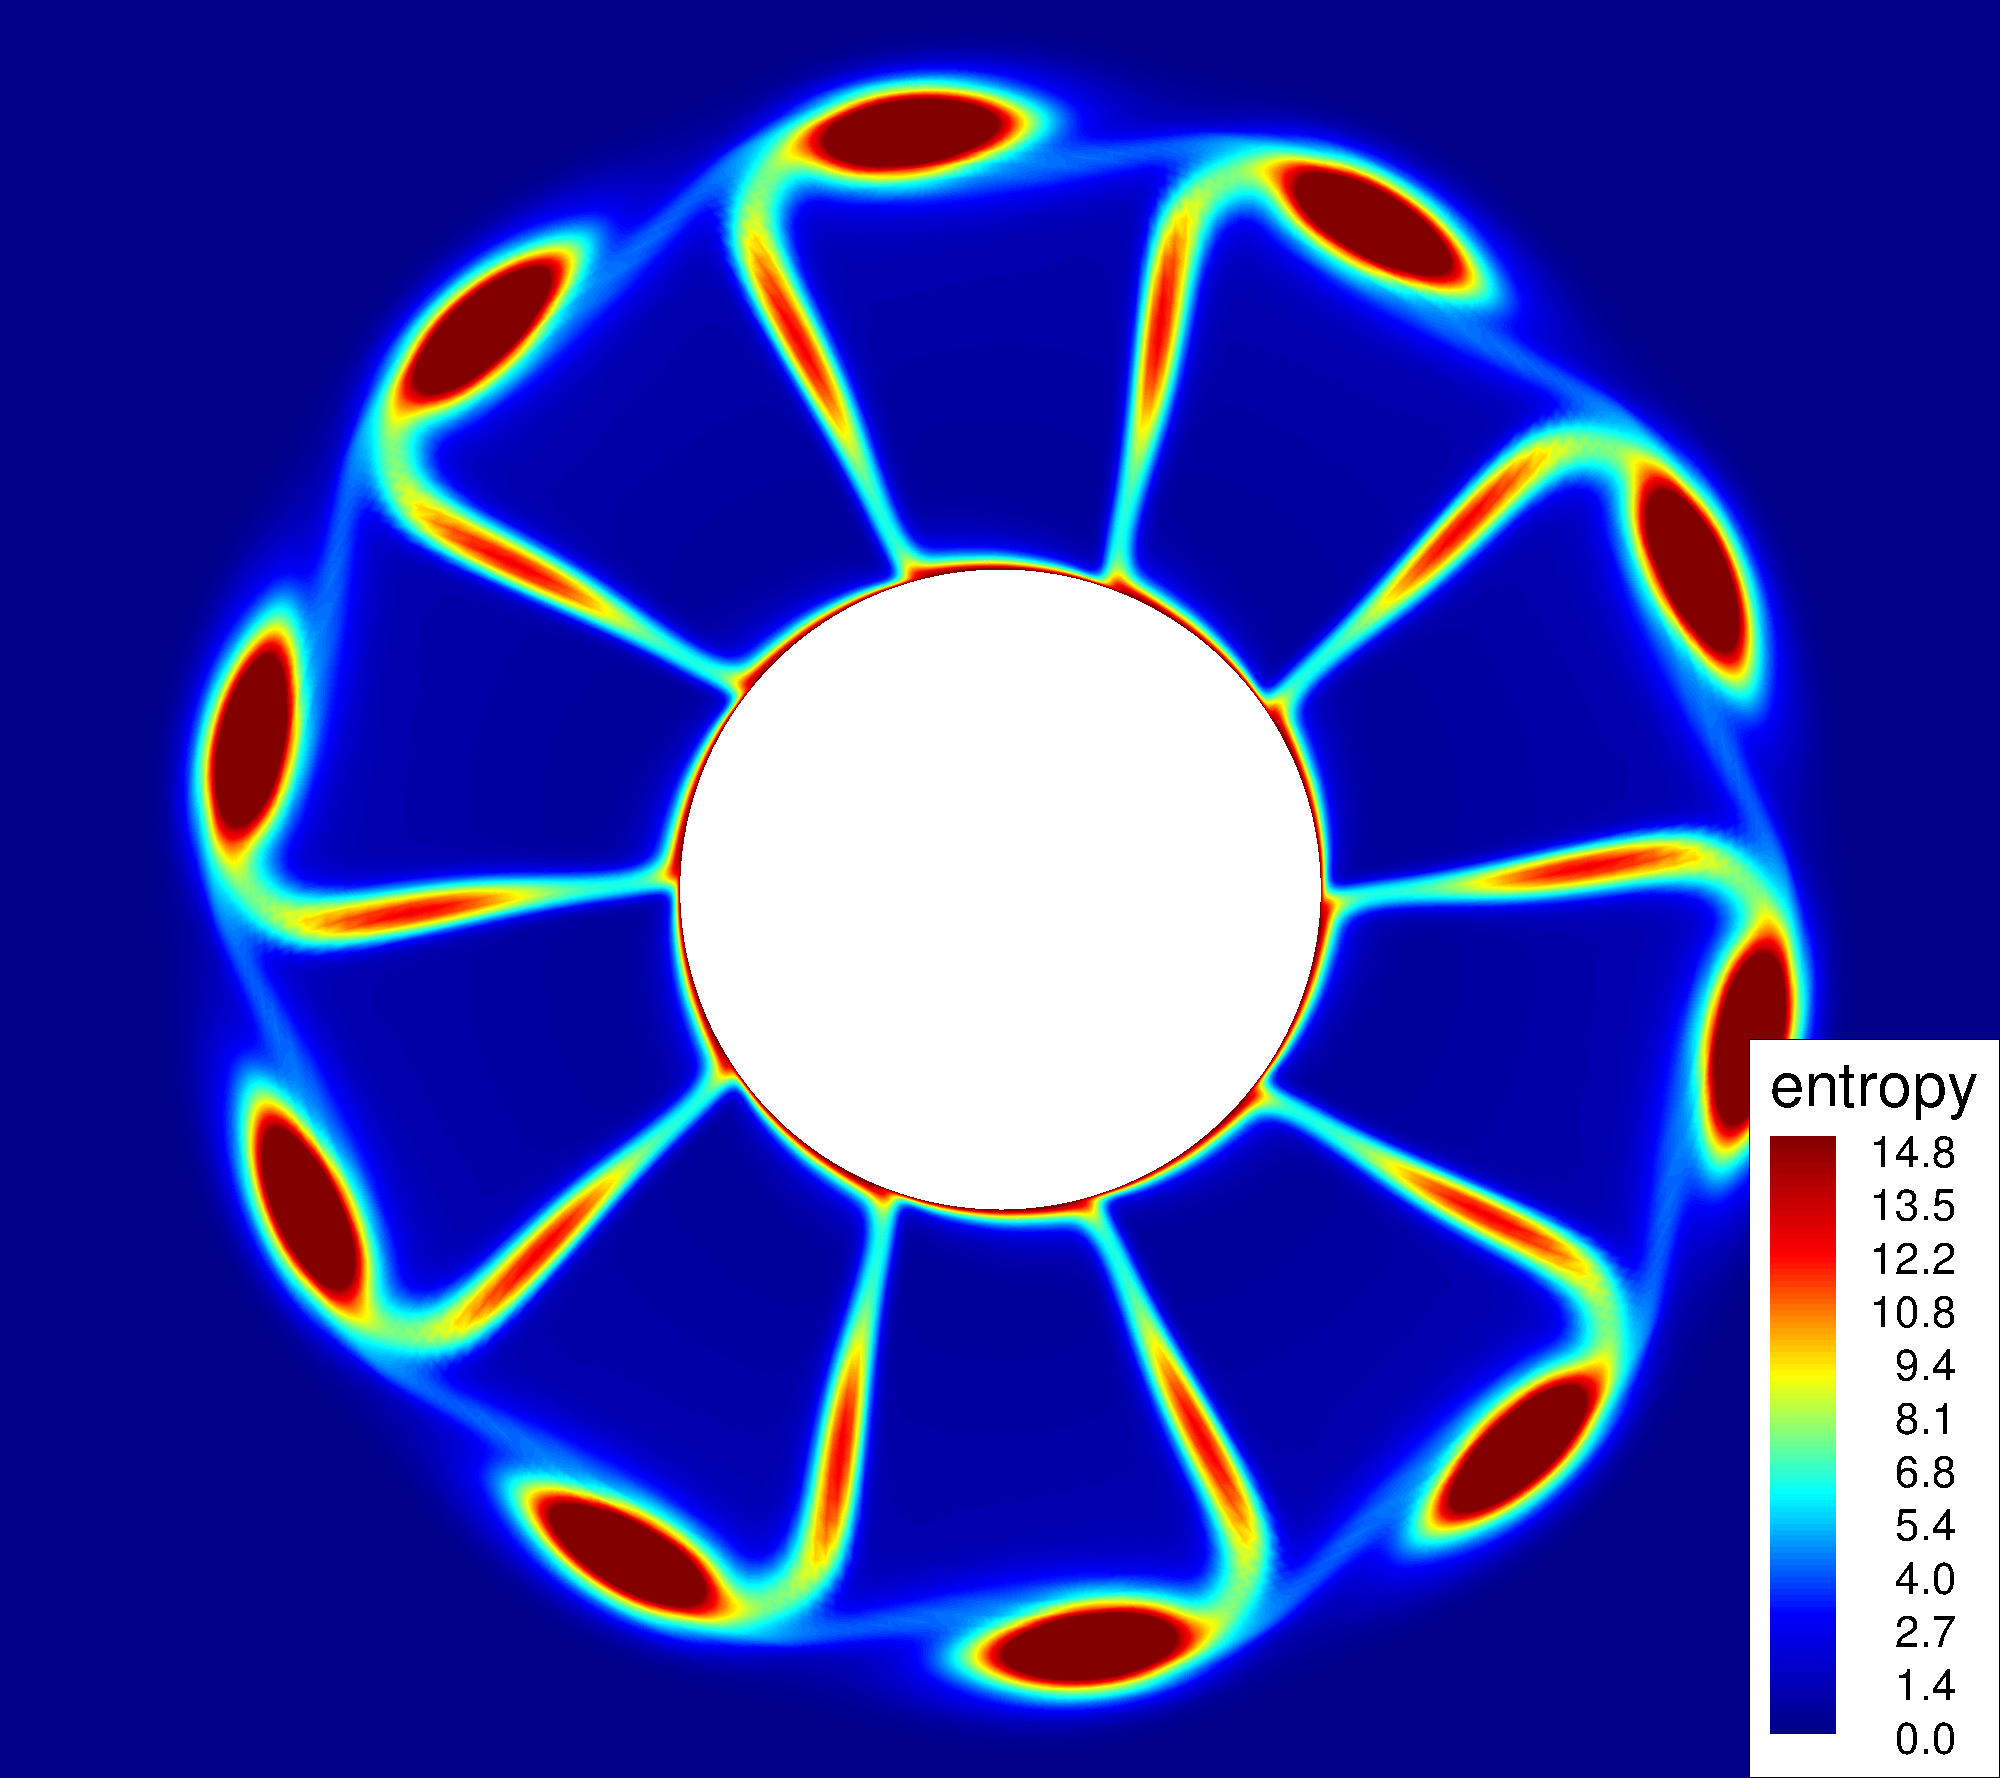
\includegraphics[width=.35\textwidth]{DREAM_LS_RANS_roe2_sa_slice_x_rear_2_entropy.png}}
  \caption{Low-speed isolated configuration: axial cuts of entropy.}
   \label{fig:dream_ls_steady_entropy}
\end{figure}

\section{Spectral convergence of the harmonic balance computations}
\label{sec:dream_ls_spectral_convergence}
%!TEX root = ../../../adrien_gomar_phd.tex

\subsection{Using the prediction tool}
\label{sub:dream_ls_conv_hb_prediction_tool}

The prediction tool based on a mixing plane computation 
described in 
Sec.~\ref{sub:prediction_tool_azimuthal_fft} is applied
to the studied configuration to evaluate the
required number of harmonics needed for the
harmonic balance approach to be converged.

To have a global insight of the energy contained in the
tangential distortion across the whole span,
the energy accumulation is plotted using a color map
in Figure~\ref{fig:DREAM_LS_RANS_ROE2_SPECTRUM_PPT}.
Three contour lines are added to ease the
interpretation: 90\%, 95\%
and 99\% of accumulated energy, corresponding to a truncation
error of respectively 30\%, 20\% and 10\%.
\begin{figure}[htp]
  \centering
  \includegraphics*[width=0.5\textwidth]{DREAM_LS_RANS_ROE2_SPECTRUM_PPT.pdf}
  \caption{Low-speed isolated configuration: prediction of the number
  of harmonics needed to simulate the configuration.}
  \label{fig:DREAM_LS_RANS_ROE2_SPECTRUM_PPT}
\end{figure}

The level of accumulated energy required 
for a computation to be rigorously converged
is difficult to estimate. 
It seems reasonable, from an engineering standpoint, to consider
that a 99\% accumulation of energy should be a good criterion.
To emphasize that,
the reconstruction of a wake as a function of four levels of cumulative
energy $E$ is depicted in Figure~\ref{fig:level_of_energy}. 
\begin{figure}[htp]
  \centering
  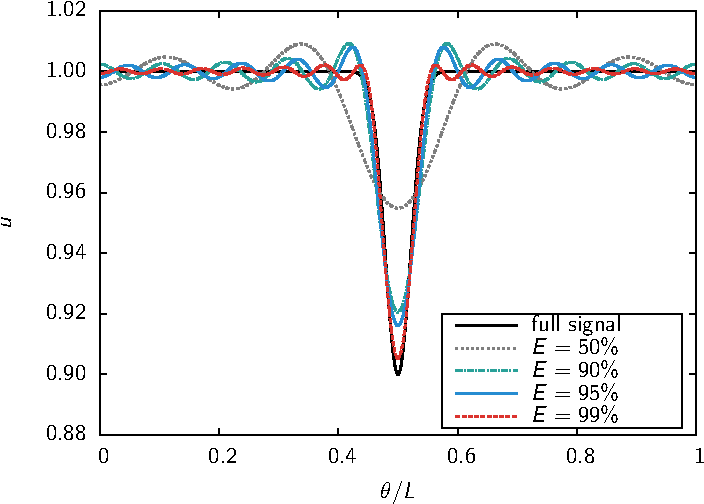
\includegraphics[width=.5\textwidth]{LEVEL_OF_ENERGY_PAPER.pdf}
  \caption{Reconstructions of a wake depending on
  the energy content kept in the signal.}
  \label{fig:level_of_energy}
\end{figure}
One can see
that a reconstruction using only 50\% of the energy
leads to a signal that has neither
the right wake deficit nor the correct width. Using
90\% and 95\% of the energy improve the resulting shape
but  large secondary
oscillations remain, with a bad capture
of the wake deficit.
In opposite, by using 99\% of the energy to reconstruct
the signal, only minor
oscillations are seen but 
the wake width and deficit are recovered with more than 
95\% accuracy.
Thus, the 99\% energy threshold ensures that the wake
will be correctly transmitted to the opposite row, which is
the prior concern of this Section.

Four harmonics are needed to capture 99\% of the energy, even though
at a relative span superior to 60\%, only three harmonics would be needed.
However, as the implementation of the harmonic balance used
in this work does not allow a varying number of harmonics through the
configuration, four harmonics is supposed to be sufficient to efficiently 
represent the unsteady flow field.

\subsection{Analyzing the similarity coefficients}
\label{sub:dream_ls_conv_hb_sim_coeff}
To confirm the number of harmonics needed to ensure the convergence
of harmonic balance computations, simulations are run with up to four
harmonics. The strategy used to launch the computation is as follow:
the steady computation is used as an initial guess for the $N=1$ HB computation.
Then each new HB computation is launched with the previous one as initial
solution.

Two harmonics are actually necessary to converge the temporal mean 
of the similarity coefficients as shown 
in Tab.~\ref{tab:dream_ls_hb_conv_sim}. After that, a slight evolution of the
coefficients is still seen but represents a change lower than 0.01\%
of the $N=4$ results, hence the convergence. 
\begin{table}[htp]
  \ra{1.3} \centering
  \begin{tabular}{rc|cccc}
    \toprule
    & steady & HB $N=1$ & HB $N=2$ & HB $N=3$ & HB $N=4$ \\
    & & \multicolumn{4}{c}{\small (time average)} \\
    \midrule
    $C_T$  & $1.1319$ & $1.1334$ & $1.1330$ & $1.1330$ & $1.1329$ \\
    $C_P$  & $2.0927$ & $2.0951$ & $2.0944$ & $2.0945$ & $2.0946$ \\
    $\eta$ & $0.5726$ & $0.5727$ & $0.5726$ & $0.5726$ & $0.5725$ \\
    \bottomrule
  \end{tabular}
  \caption{Low-speed isolated configuration: analysis of the number of harmonics
  required to capture the time average similarity coefficients.}
  \label{tab:dream_ls_hb_conv_sim}
\end{table}
Note that a steady computation is sufficient to retrieve
the temporal mean value of the similarity coefficients.
In fact, on this variables, a maximum of 0.1\% difference is observed by
comparing the mixing plane and harmonic balance results.

\subsection{Analyzing the blade response}
\label{sub:dream_ls_conv_hb_blade_response}
Of course, analyzing integrated results to assess the convergence  of
a computation is a primarily step that should be complemented with
a local analysis. In this way, a discrete Fourier transform is
performed to analyze the first harmonic of the static pressure on the 
rear rotor blades. Due to the passing
of the front rotor wakes, these blades will experience a
high level of unsteadinesses. It is therefore considered as a
bottleneck in the convergence of the HB computations, hence its analysis.
The results are shown in 
Figure~\ref{fig:dream_ls_hb_blade_response_conv}. 
\begin{figure}[htp]
 \ra{1.3} \centering
 \begin{tabular}{r|cccc}
   \toprule
   & \multicolumn{2}{c}{mean} & \multicolumn{2}{c}{1\textsuperscript{st} harmonic} \\
   & \multicolumn{2}{c}{
        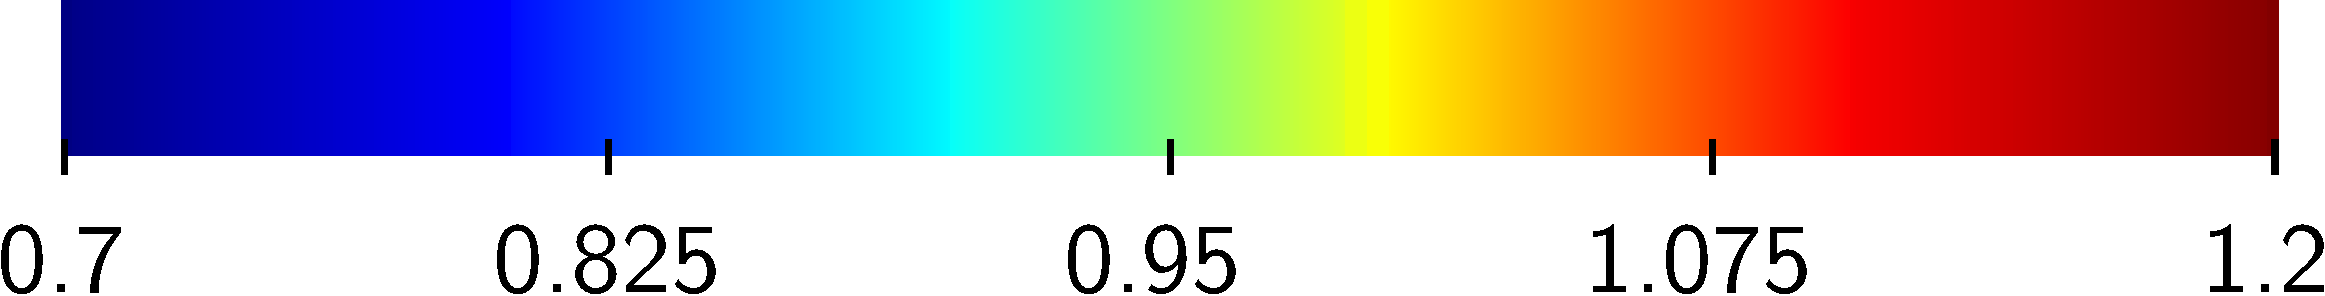
\includegraphics[width=0.22\textwidth]{dream_ls_blade_resp_scale_mean.pdf}} 
   & \multicolumn{2}{c}{
        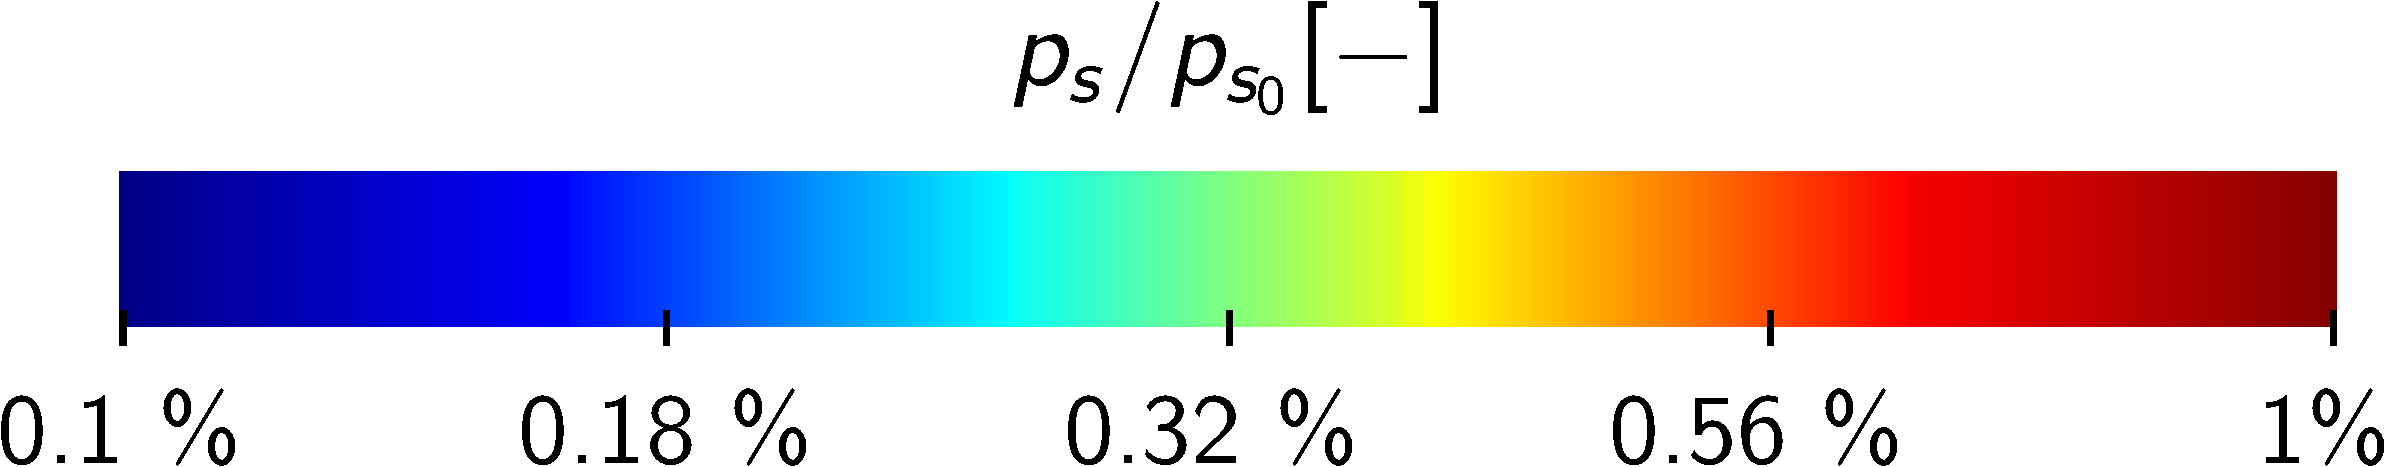
\includegraphics[width=0.22\textwidth]{dream_ls_blade_resp_scale_H01_rear.pdf}} \\
   \midrule
   \rotatebox{90}{\quad\quad\quad steady} 
   & 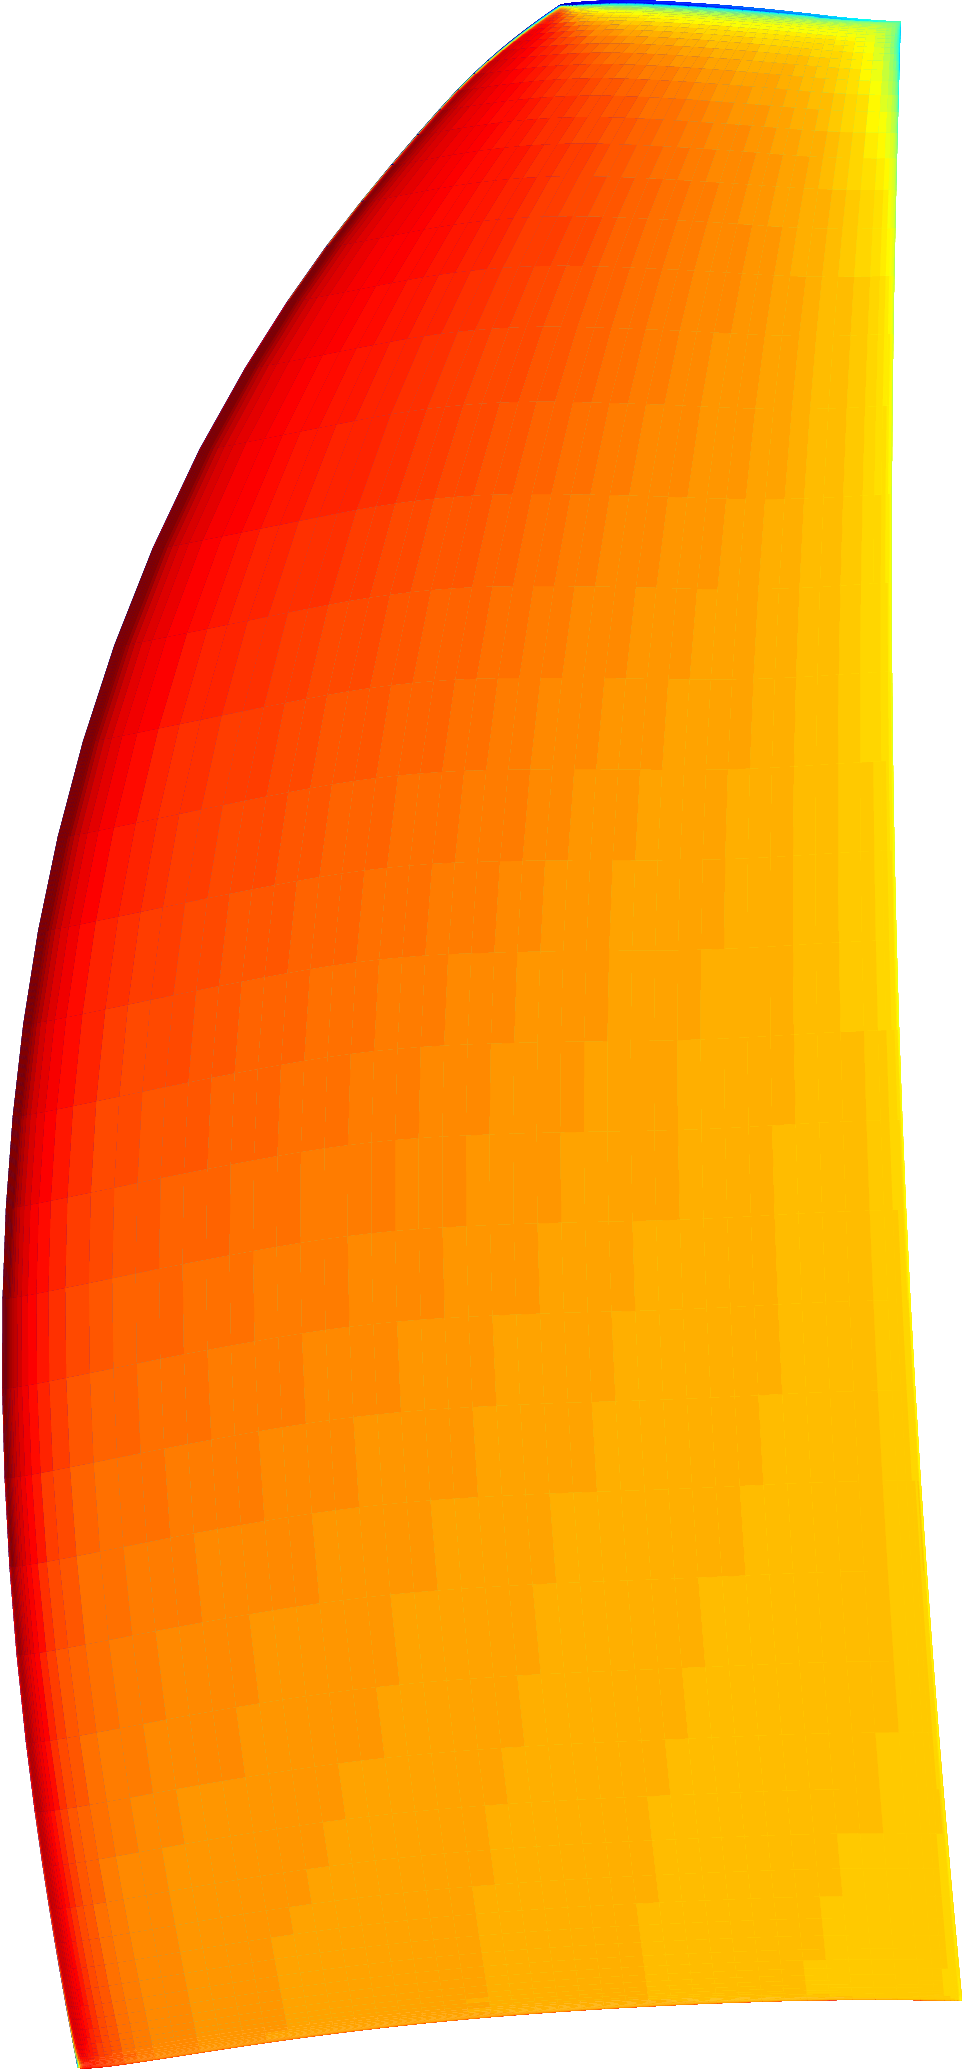
\includegraphics[width=0.10\textwidth]{DREAM_LS_RANS_roe2_sa_blade_response_rear_PS.png}
   & 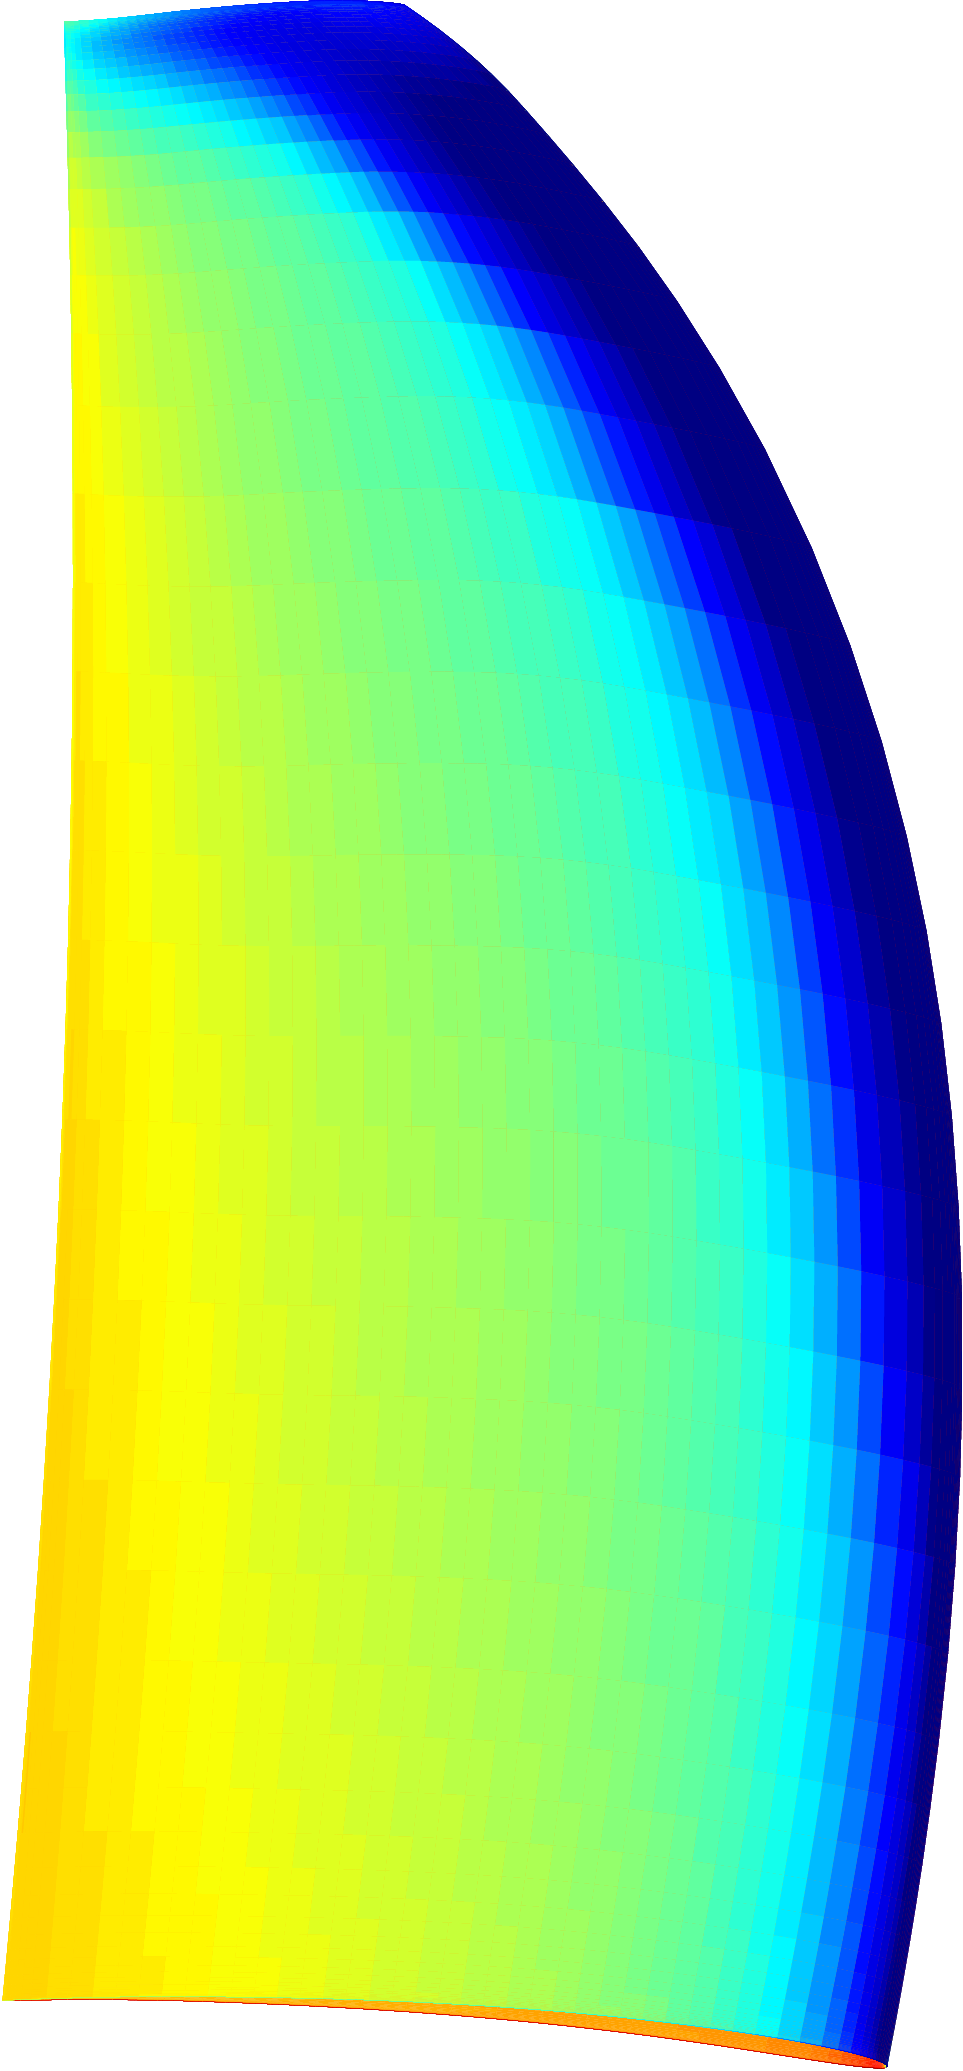
\includegraphics[width=0.10\textwidth]{DREAM_LS_RANS_roe2_sa_blade_response_rear_SS.png}
   &   &\\
   \rotatebox{90}{\quad\quad HB $N=1$} 
   & 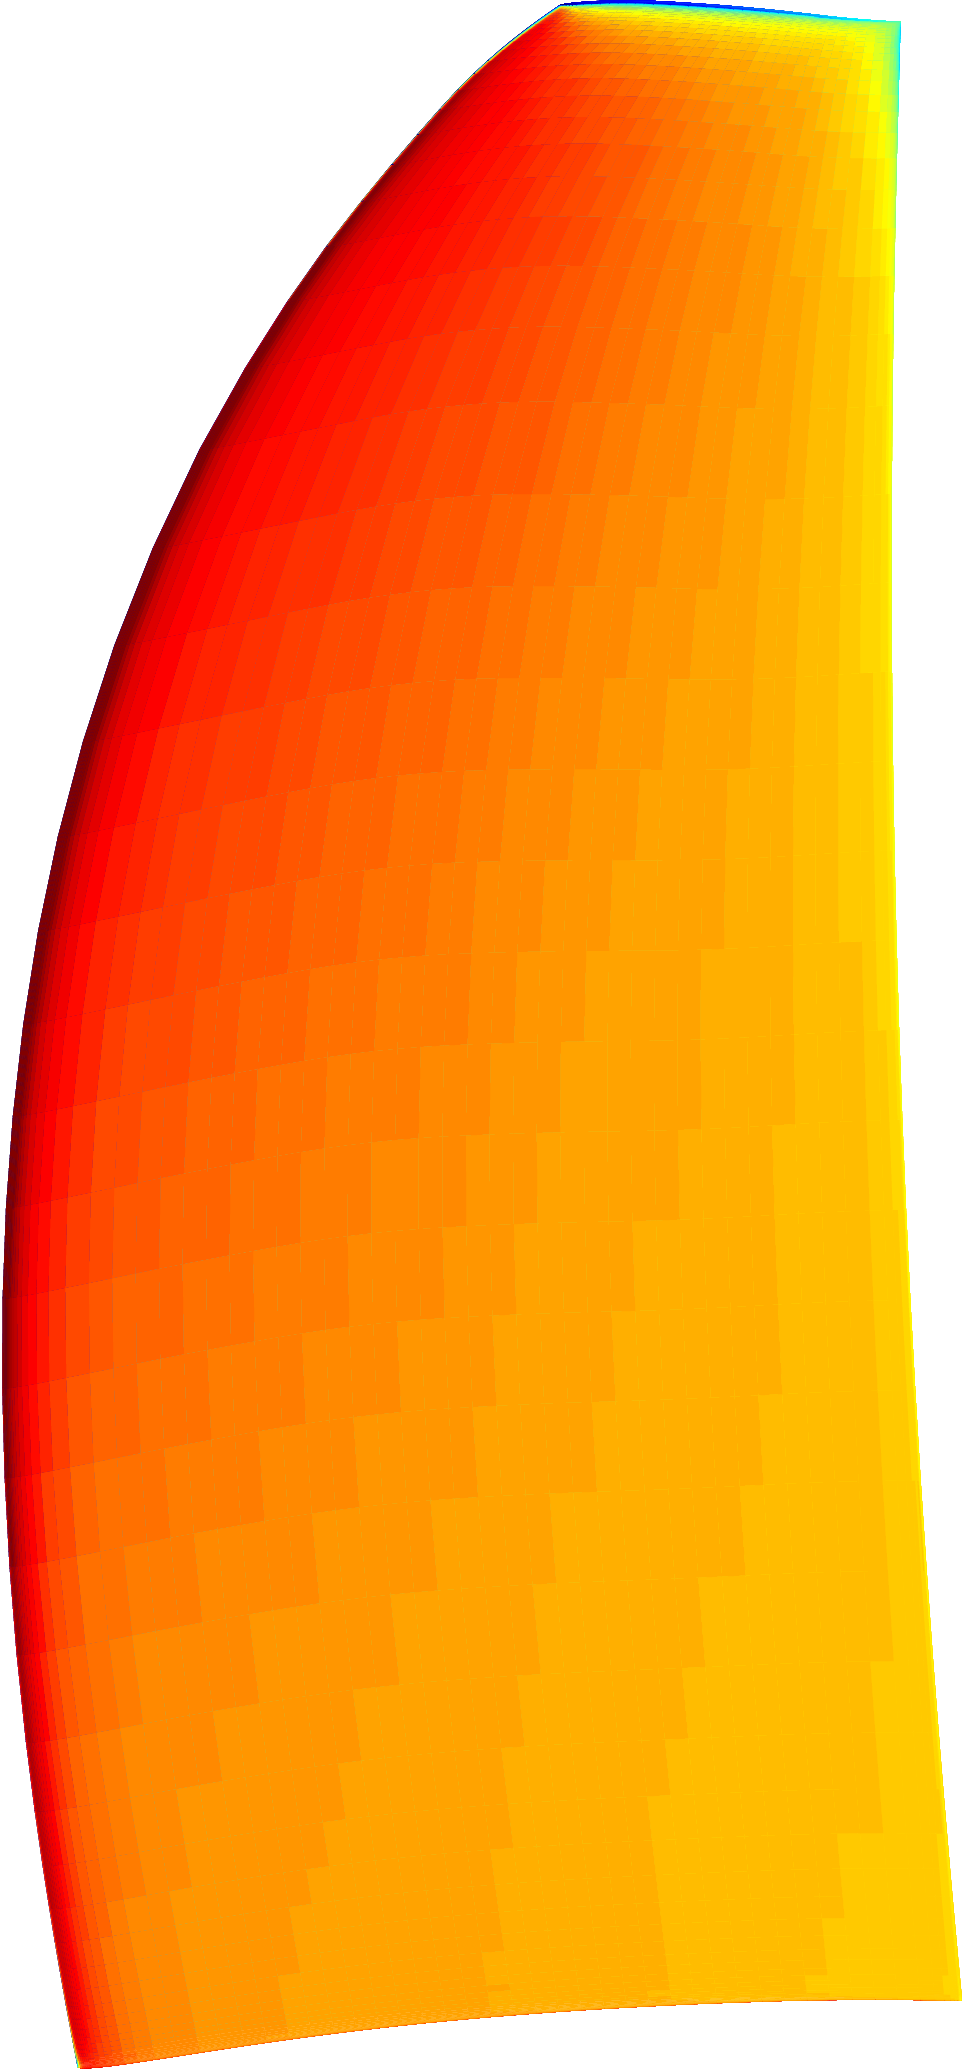
\includegraphics[width=0.10\textwidth]{DREAM_LS_TSM_N1_roe2_sa_blade_response_rear_mean_PS.png}
   & 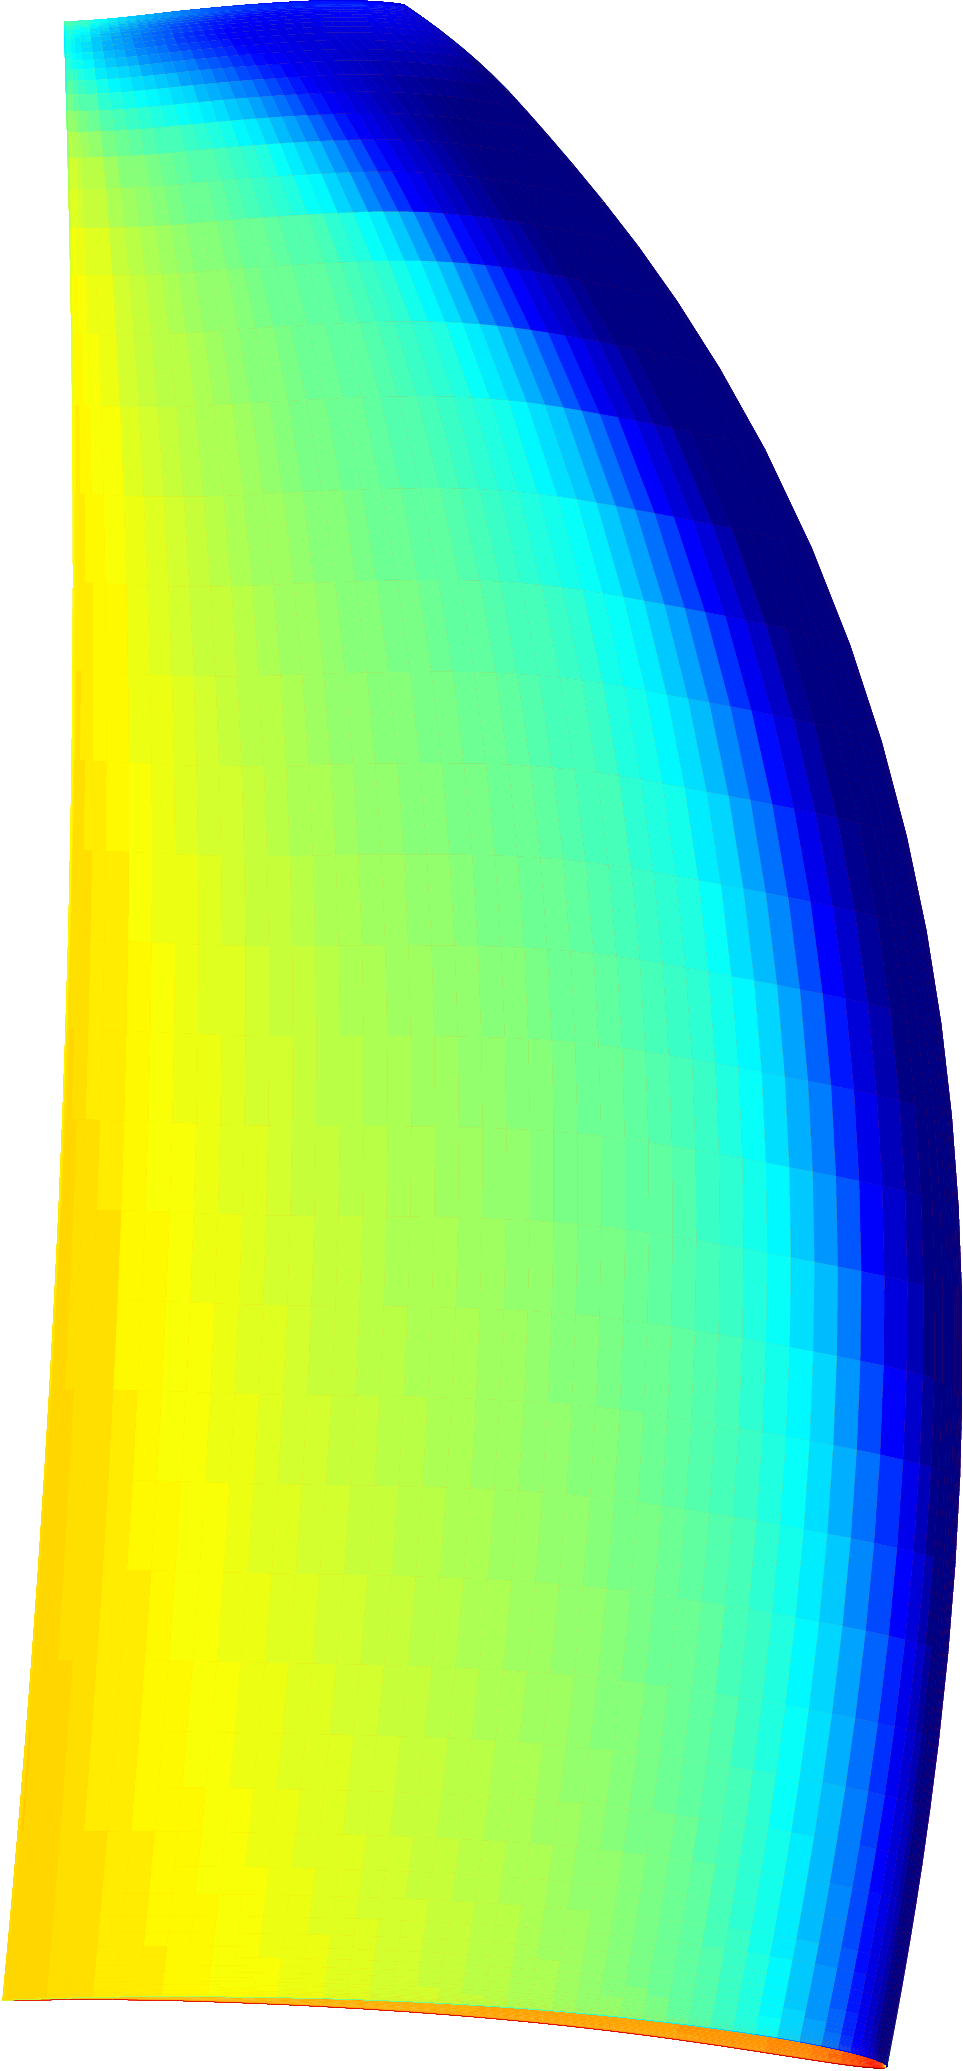
\includegraphics[width=0.10\textwidth]{DREAM_LS_TSM_N1_roe2_sa_blade_response_rear_mean_SS.png}
   & 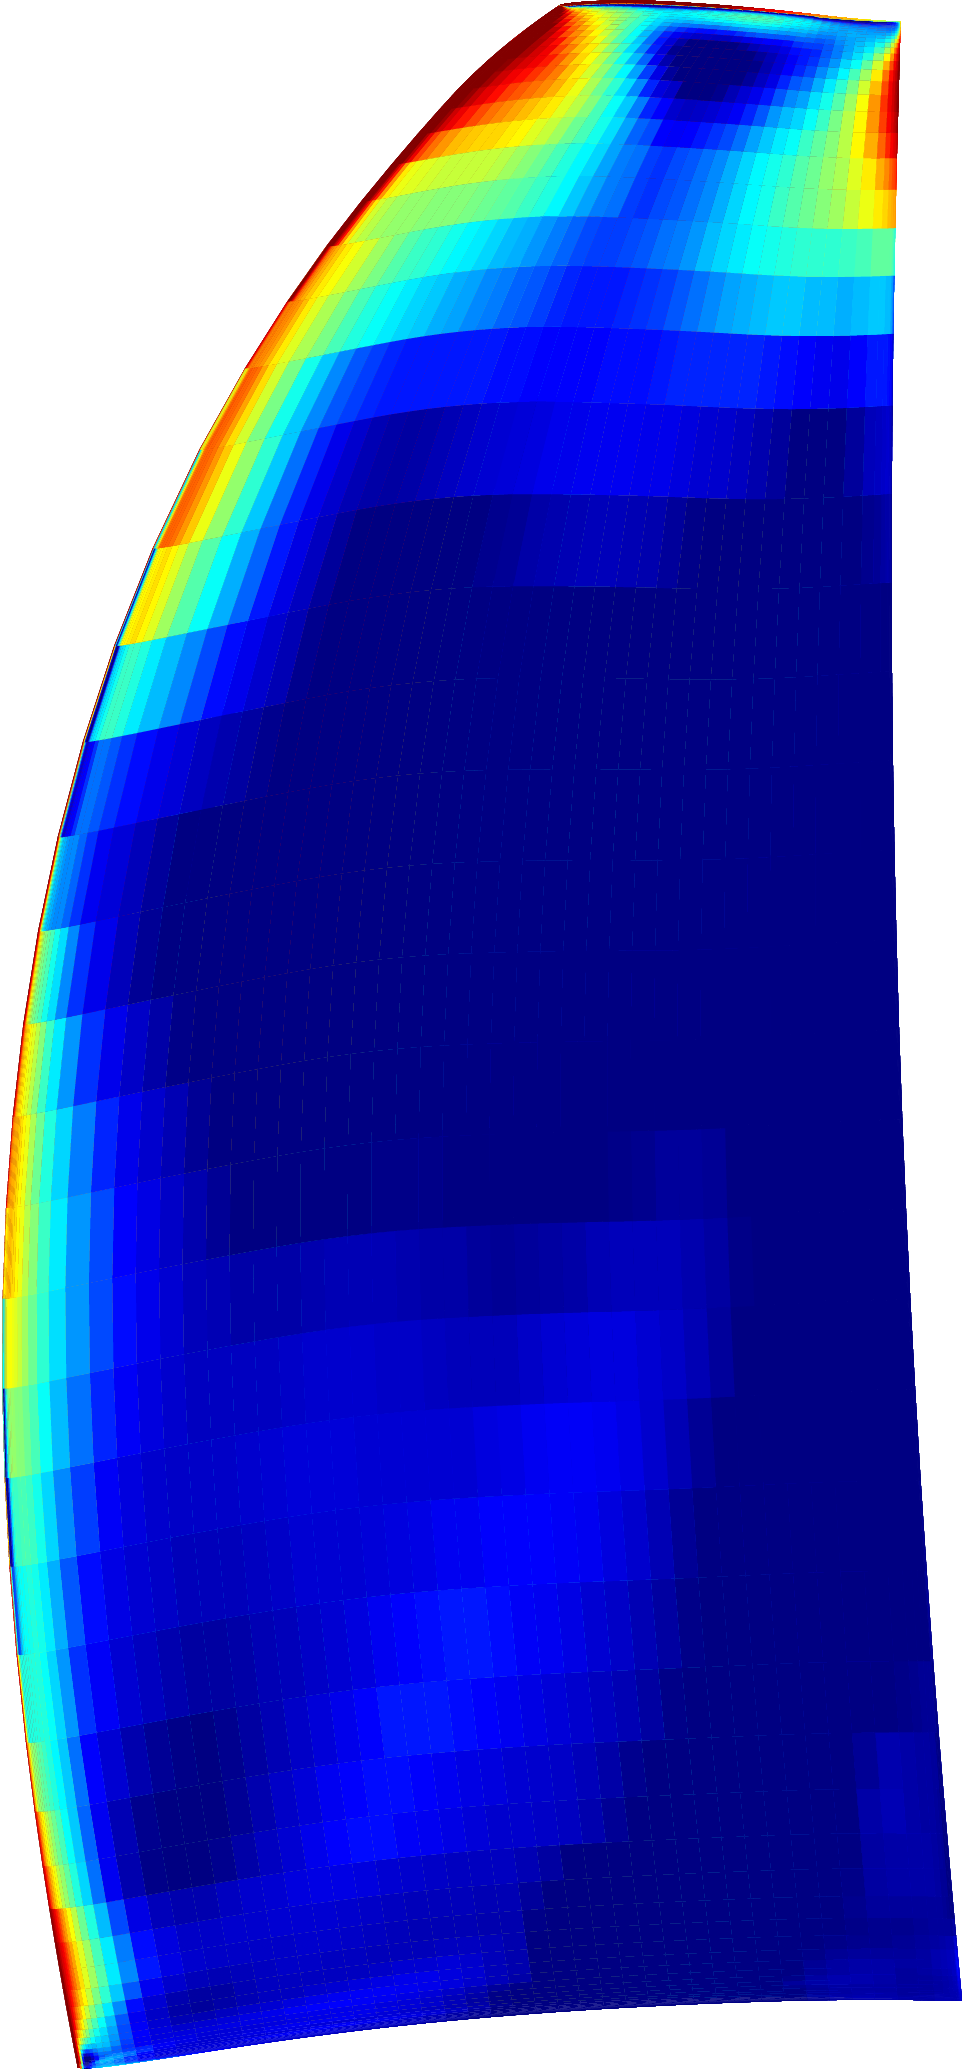
\includegraphics[width=0.10\textwidth]{DREAM_LS_TSM_N1_roe2_sa_blade_response_rear_H01_PS.png}
   & 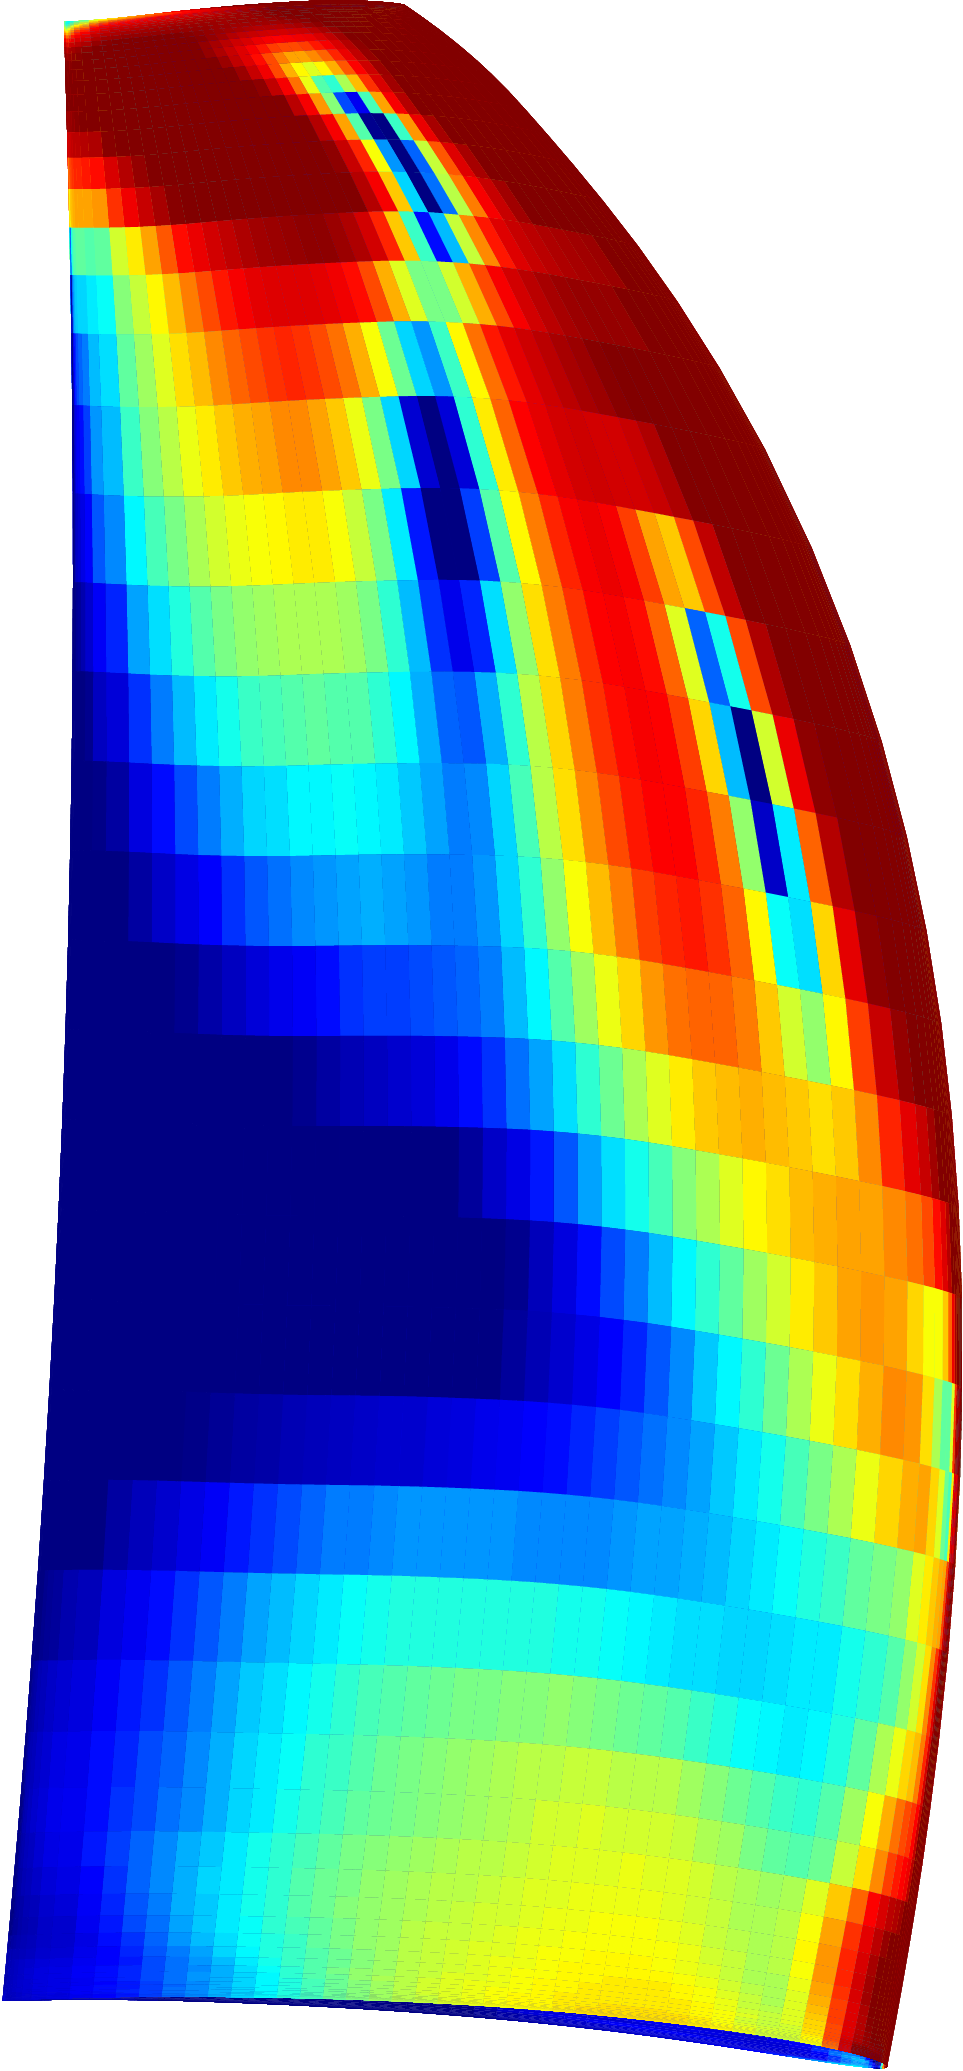
\includegraphics[width=0.10\textwidth]{DREAM_LS_TSM_N1_roe2_sa_blade_response_rear_H01_SS.png} \\
   \rotatebox{90}{\quad\quad HB $N=2$} 
   & 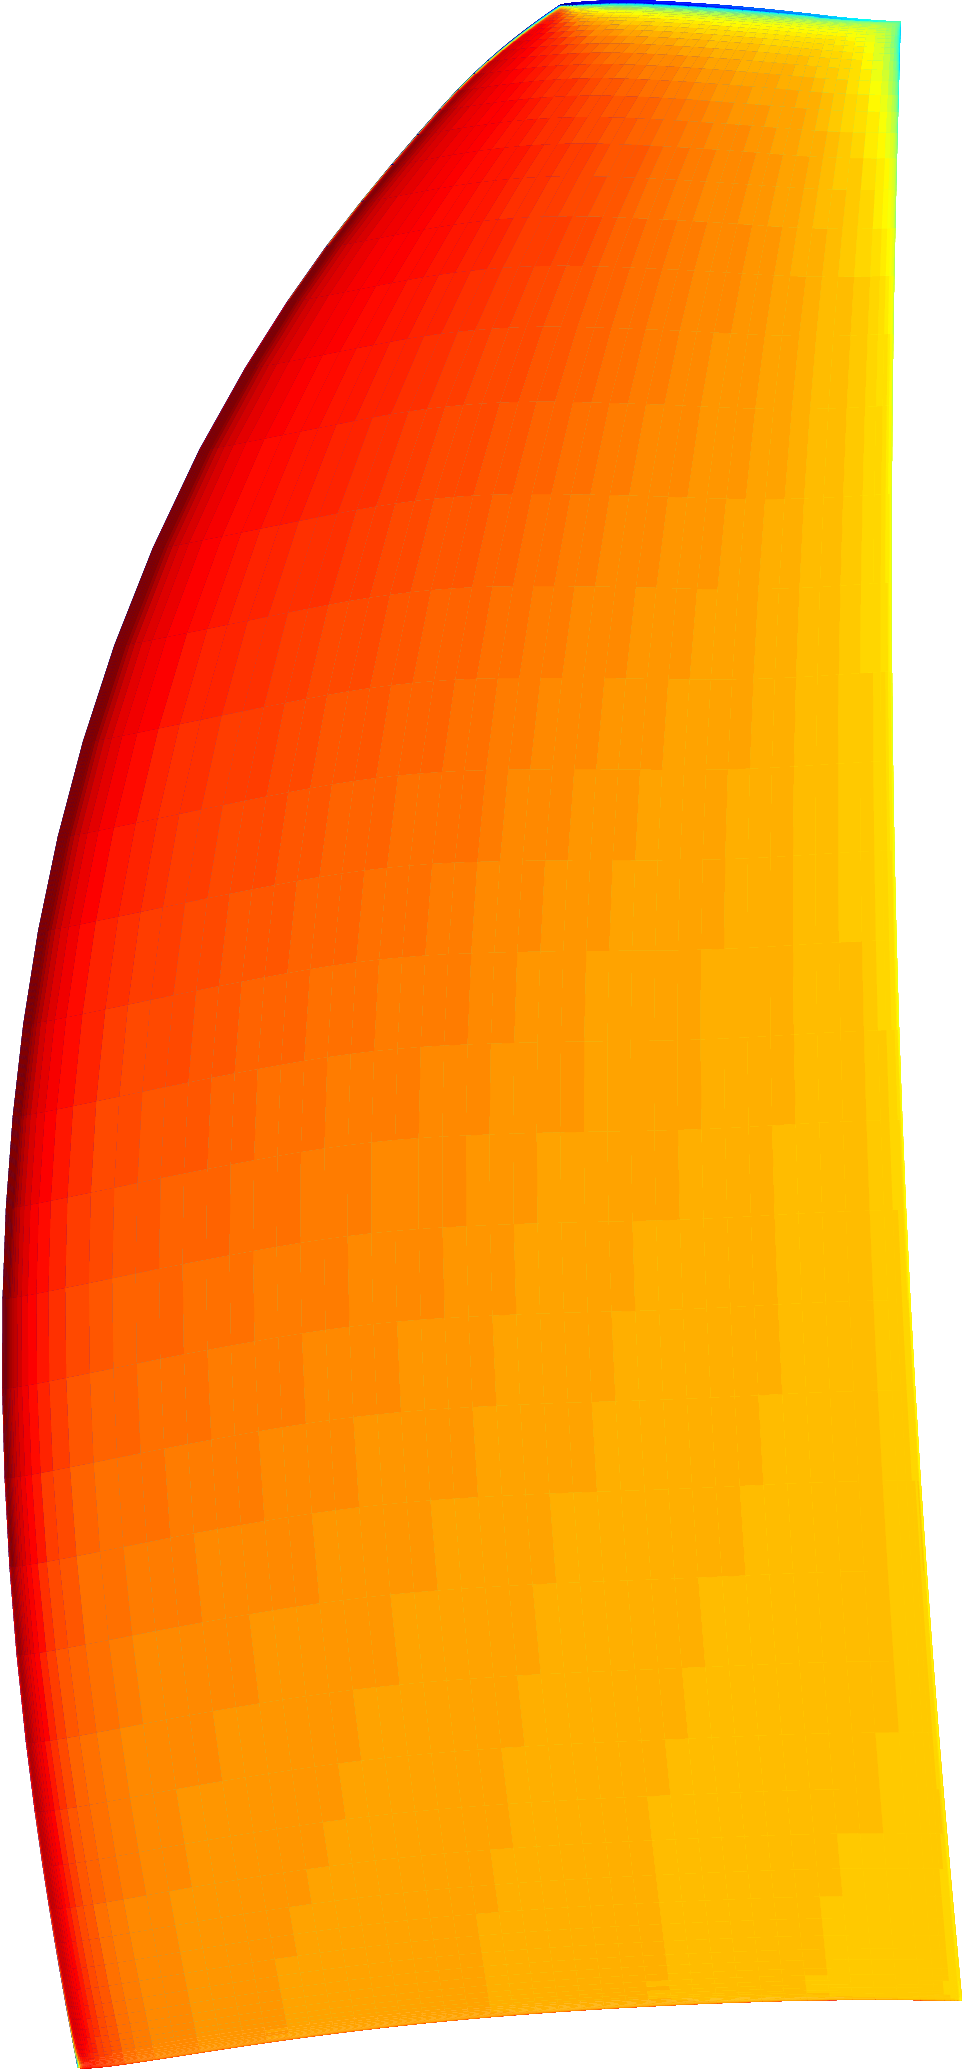
\includegraphics[width=0.10\textwidth]{DREAM_LS_TSM_N2_roe2_sa_blade_response_rear_mean_PS.png}
   & 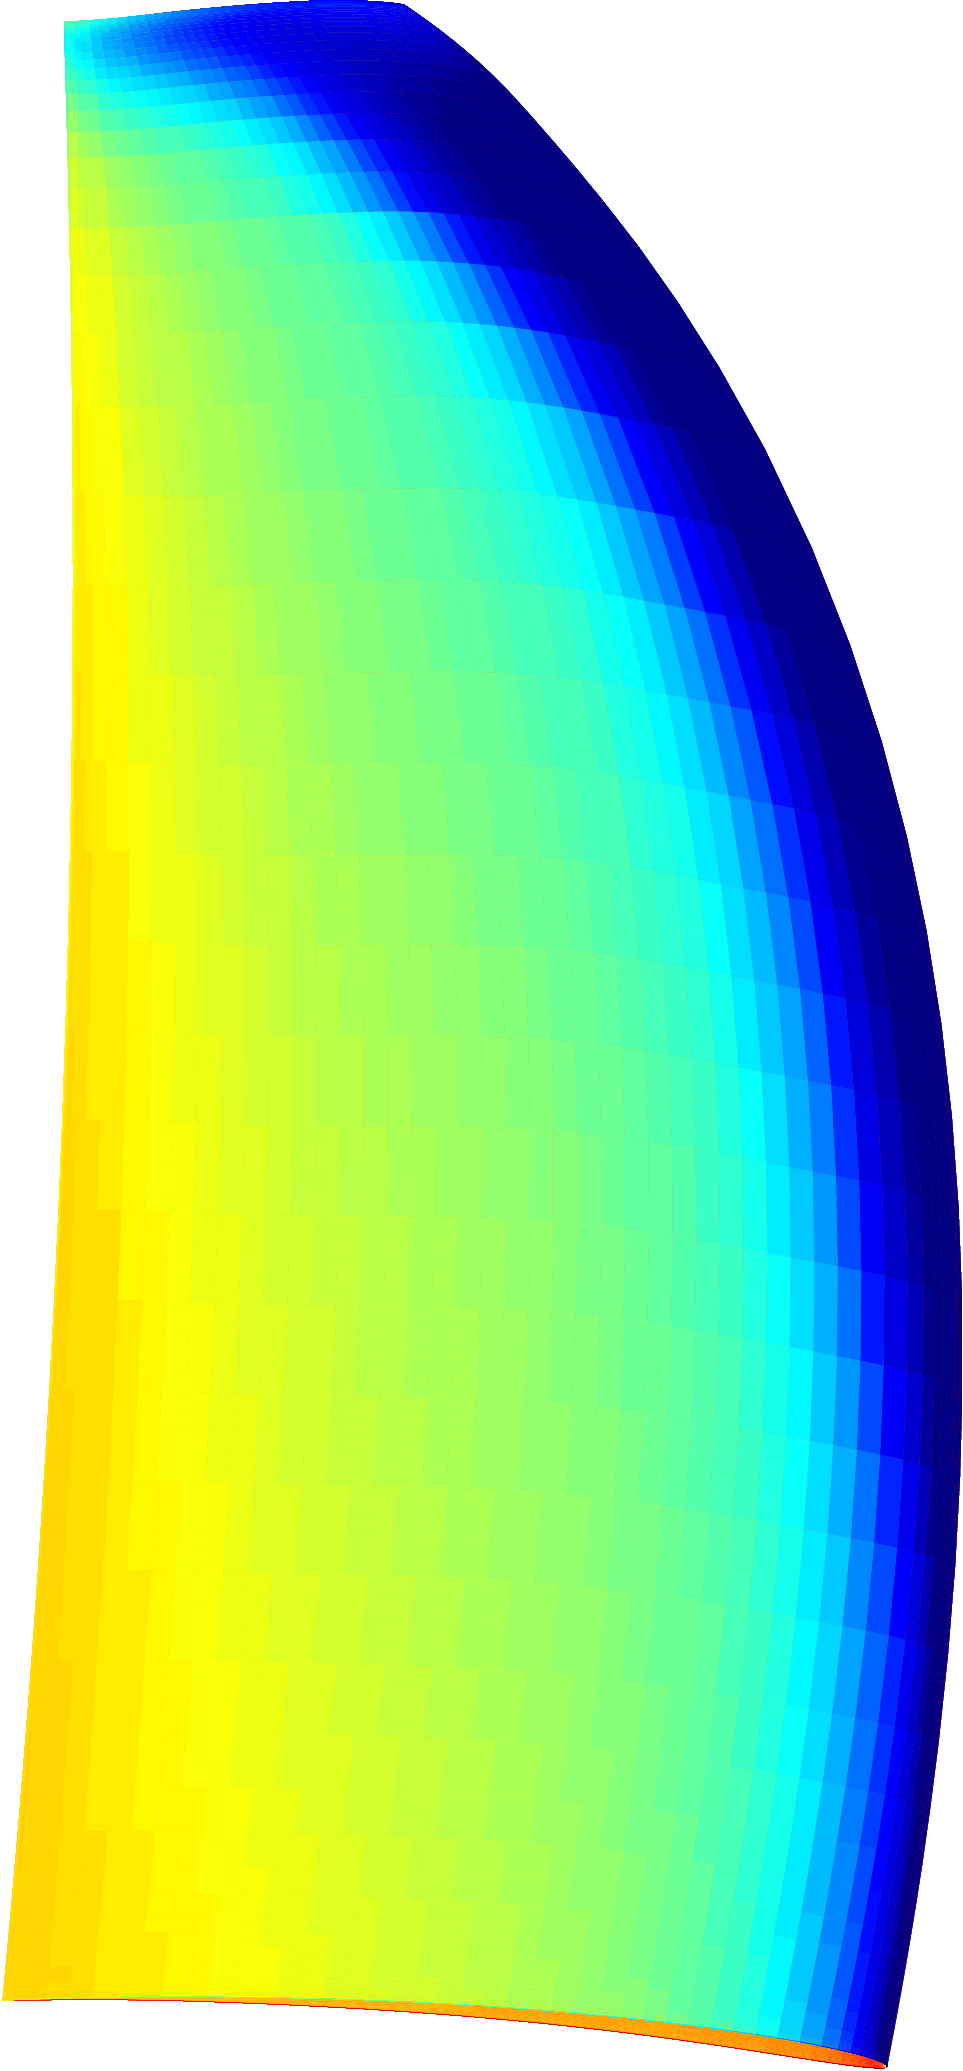
\includegraphics[width=0.10\textwidth]{DREAM_LS_TSM_N2_roe2_sa_blade_response_rear_mean_SS.png}
   & 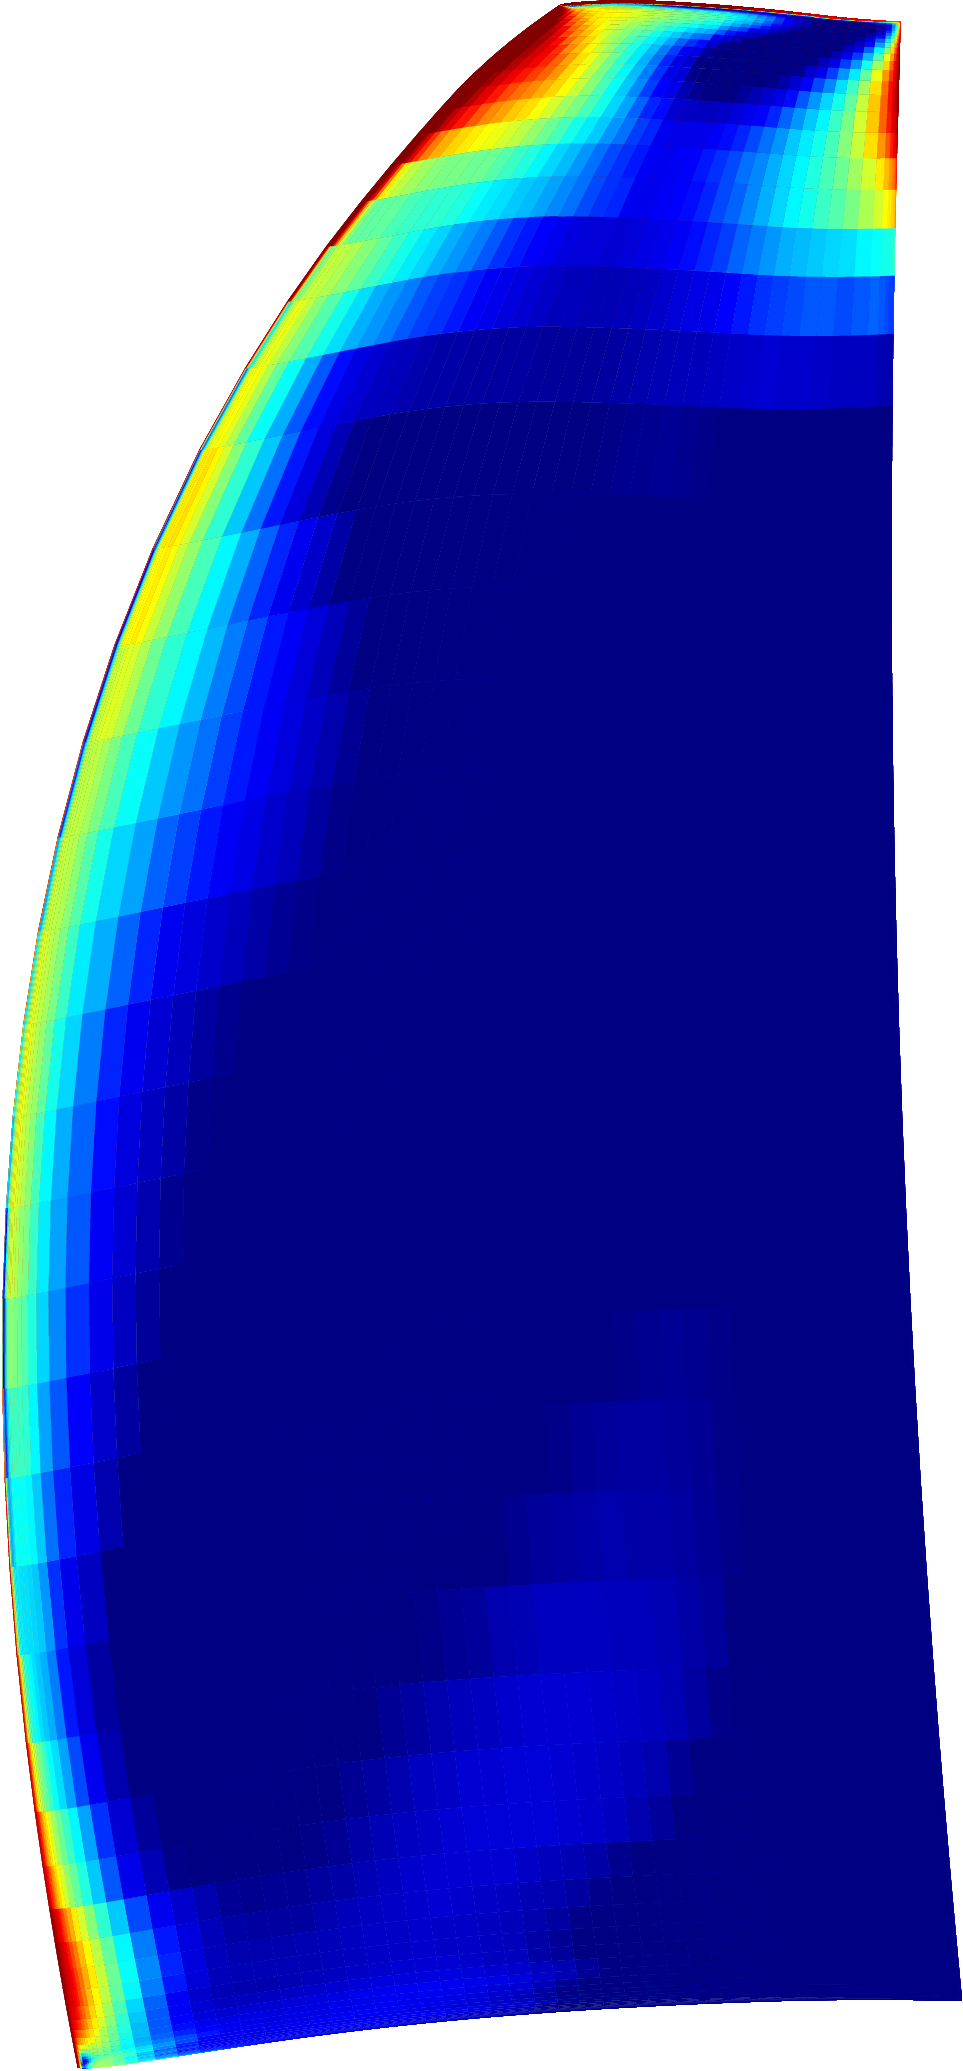
\includegraphics[width=0.10\textwidth]{DREAM_LS_TSM_N2_roe2_sa_blade_response_rear_H01_PS.png}
   & 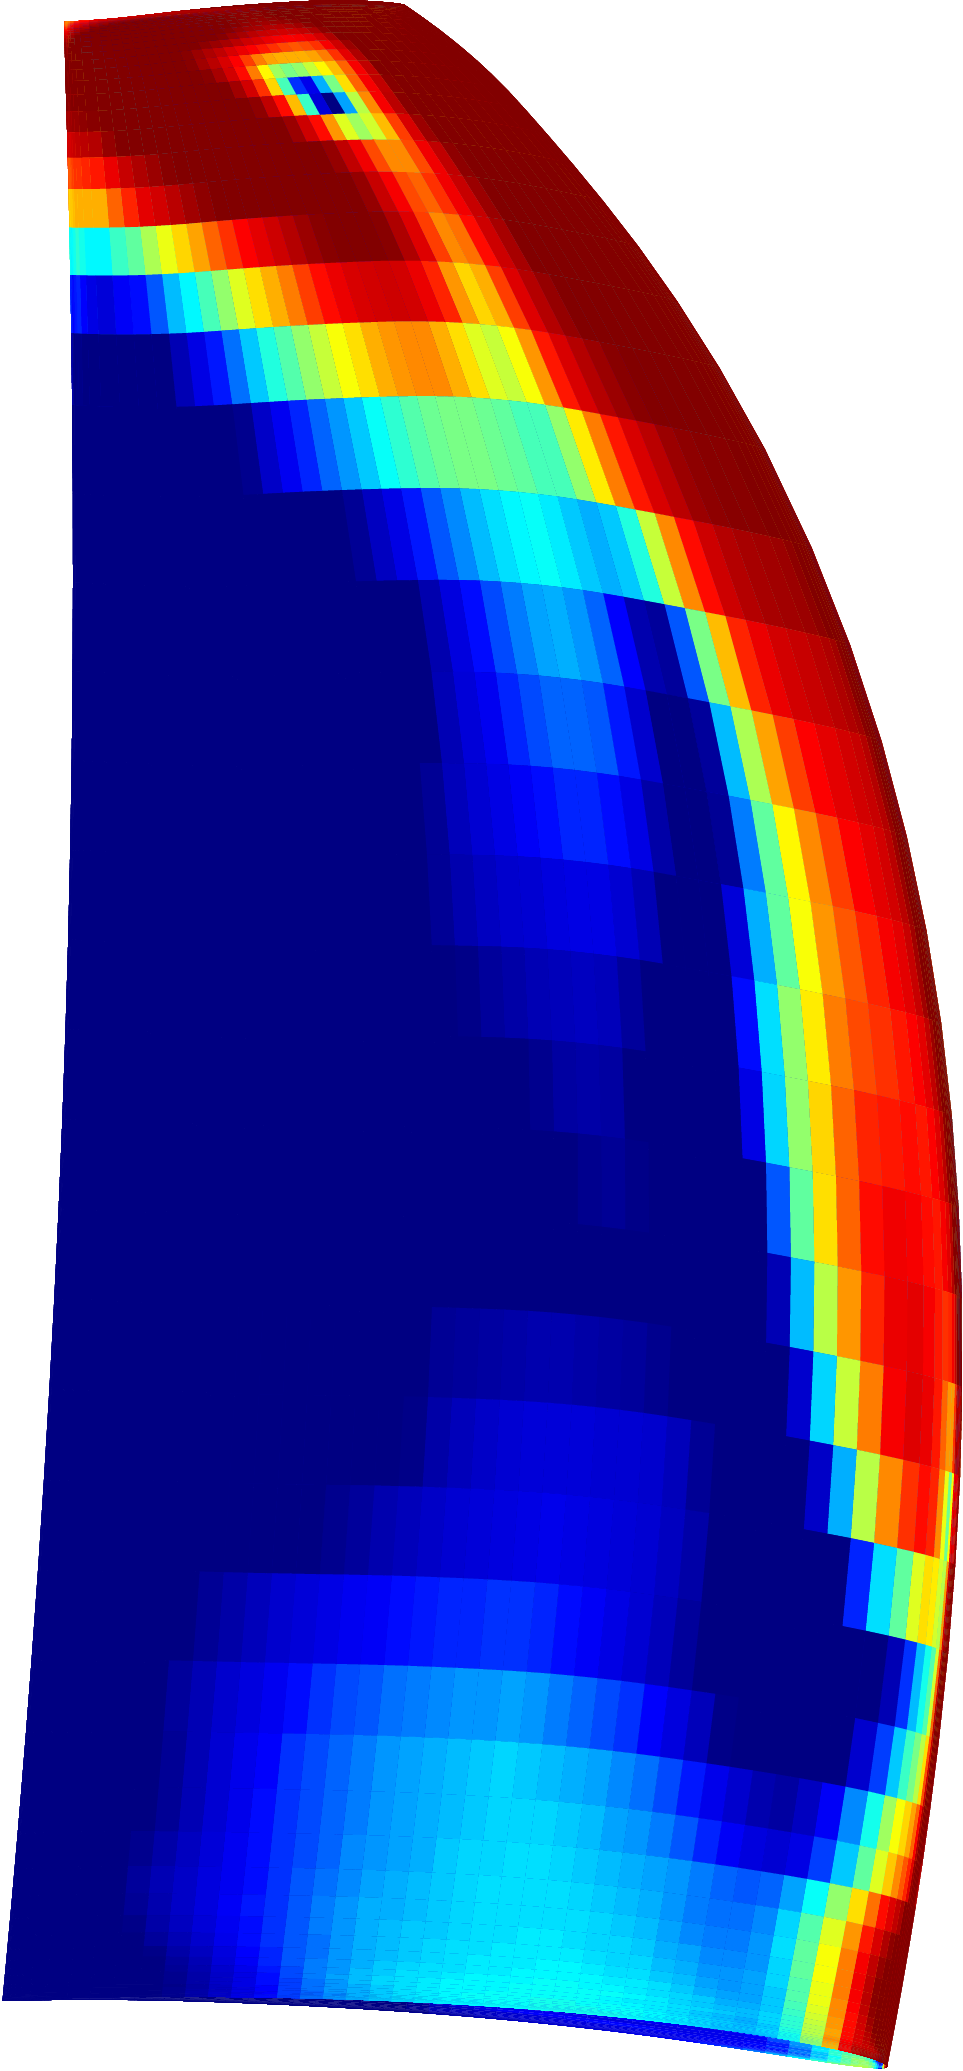
\includegraphics[width=0.10\textwidth]{DREAM_LS_TSM_N2_roe2_sa_blade_response_rear_H01_SS.png} \\
   \rotatebox{90}{\quad\quad HB $N=3$} 
   & 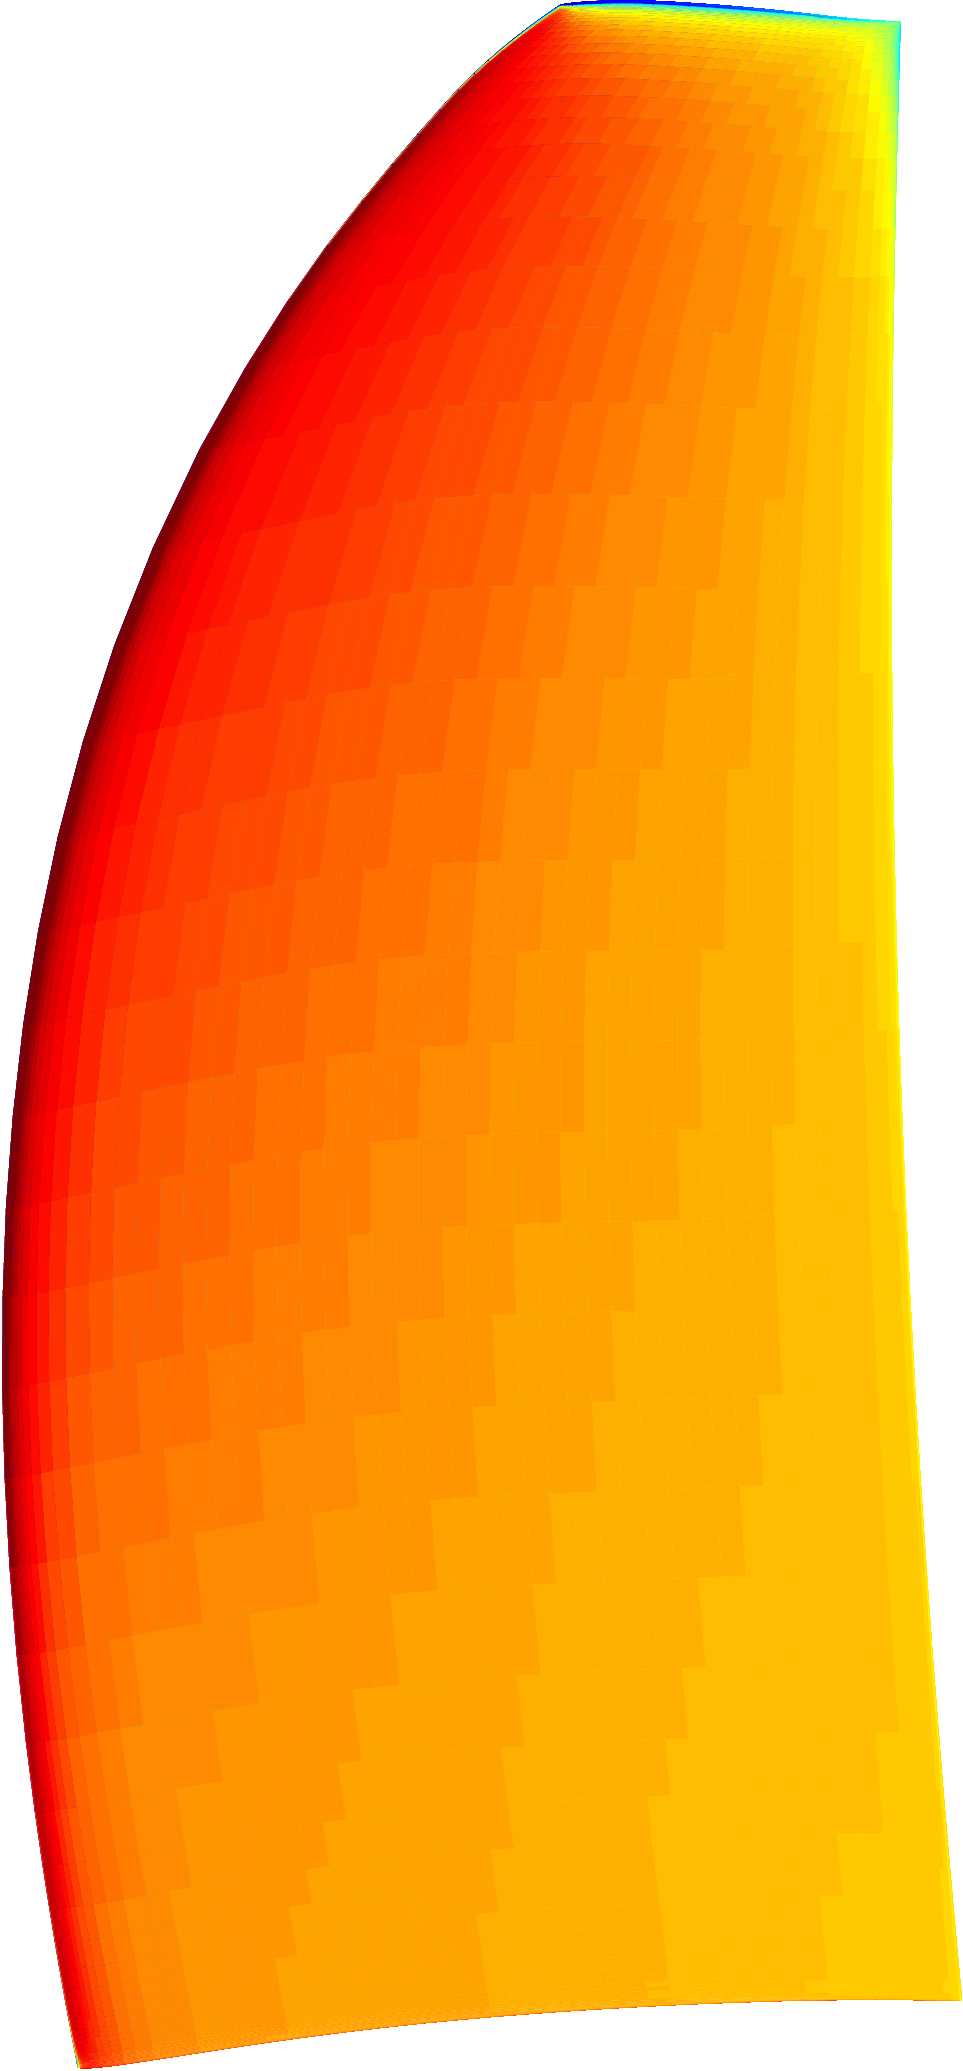
\includegraphics[width=0.10\textwidth]{DREAM_LS_TSM_N3_roe2_sa_blade_response_rear_mean_PS.png}
   & 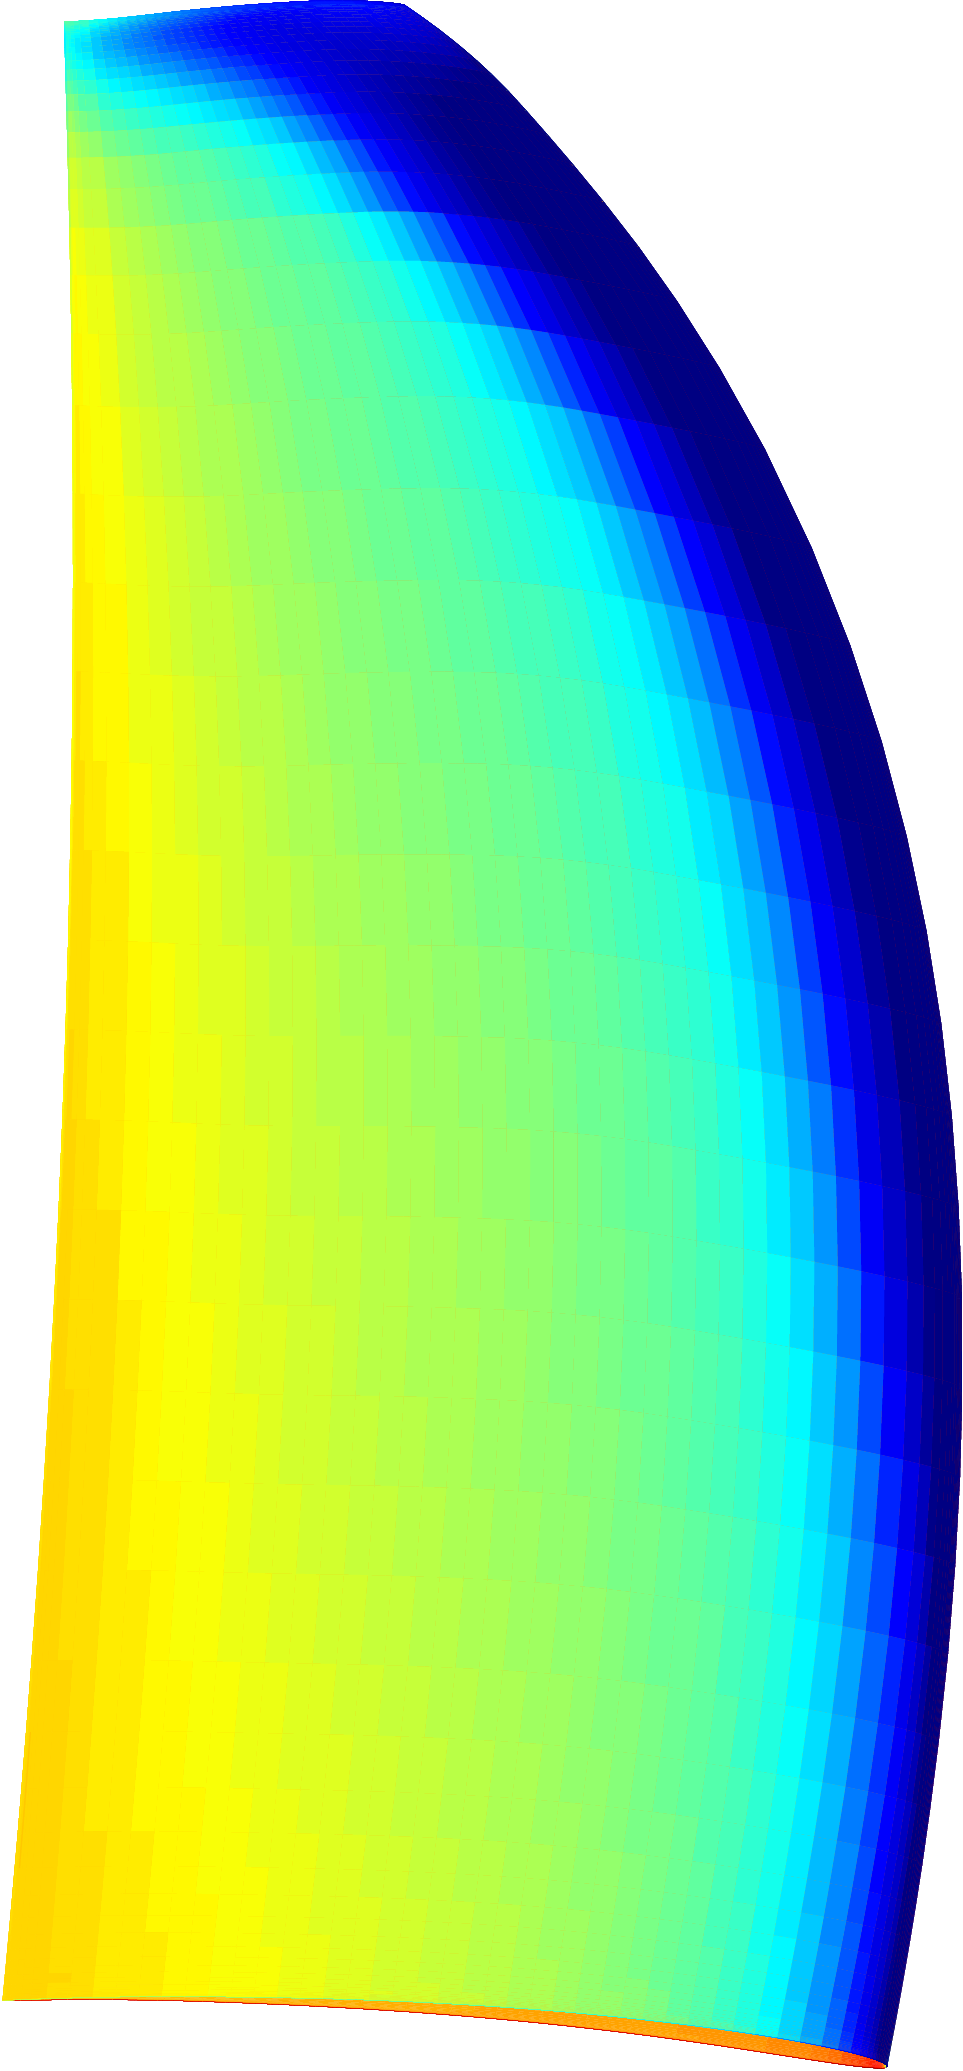
\includegraphics[width=0.10\textwidth]{DREAM_LS_TSM_N3_roe2_sa_blade_response_rear_mean_SS.png}
   & 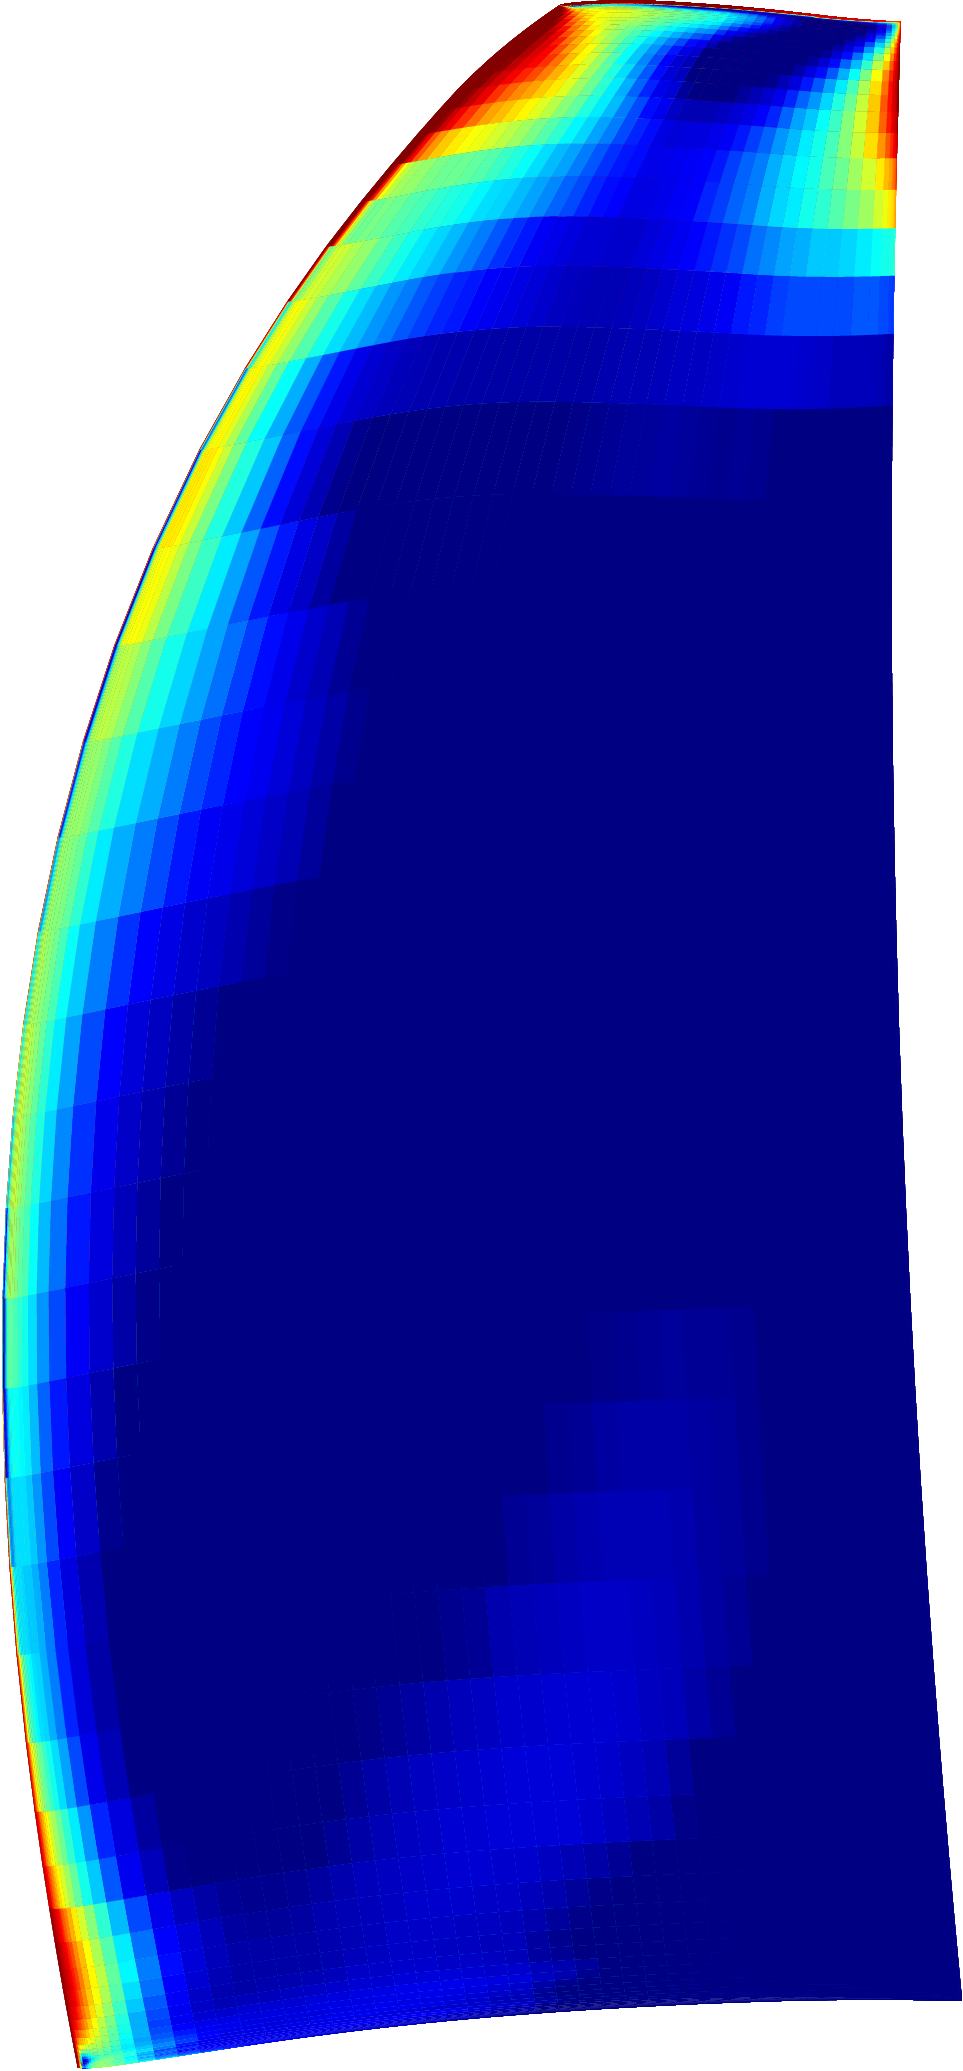
\includegraphics[width=0.10\textwidth]{DREAM_LS_TSM_N3_roe2_sa_blade_response_rear_H01_PS.png}
   & \includegraphics[width=0.10\textwidth]{DREAM_LS_TSM_N3_roe2_sa_blade_response_rear_H01_SS.png} \\
   \rotatebox{90}{\quad\quad HB $N=4$} 
   & \includegraphics[width=0.10\textwidth]{DREAM_LS_TSM_N4_roe2_sa_blade_response_rear_mean_PS.png}
   & \includegraphics[width=0.10\textwidth]{DREAM_LS_TSM_N4_roe2_sa_blade_response_rear_mean_SS.png}
   & \includegraphics[width=0.10\textwidth]{DREAM_LS_TSM_N4_roe2_sa_blade_response_rear_H01_PS.png}
   & \includegraphics[width=0.10\textwidth]{DREAM_LS_TSM_N4_roe2_sa_blade_response_rear_H01_SS.png} \\
   \bottomrule
 \end{tabular}
 \caption{Low-speed isolated configuration: analysis of the number of harmonics
  required to capture the harmonic response of the rear rotor blades.}
 \label{fig:dream_ls_hb_blade_response_conv}
\end{figure}

Only one harmonic is needed to converge the time-average value on the
rear rotor blades. Actually, the steady computation already gave a good prediction
of this time averaged value. This is due to the range on which this
low-speed CROR configuration operates. The Mach number is almost within the
incompressible range. As such, the non-linearities of the Navier--Stokes equations
remains small and steady approaches give good results.

Two to three harmonics are needed to converge the first harmonic 
pressure response on the rear rotor blade. This is a rough estimation
as a small convergence of the
harmonic pressure rise on the suction side of the blade between HB $N=2$, 
$N=3$ and $N=4$ computations can be seen. 

\subsection{Analyzing the radial cuts}
\label{sub:dream_ls_conv_hb_slice_r}
The final assessment of the convergence is done on radial cuts
of entropy made at 75\% of the height of the rear rotor blade.
This is the region where the blades is most likely to be
highly loaded, hence the choice of this span.
The entropy spurious waves vanishes when computing the HB $N=4$ even though
the HB $N=3$ computation give a relatively smooth entropy field.
\begin{figure}[htp]
  \centering
  \subfigure[HB $N=1$]{
  \includegraphics[width=.35\textwidth]{DREAM_LS_TSM_N1_roe2_sa_slice_r_75_entropy.png}}
  \subfigure[HB $N=2$]{
  \includegraphics[width=.35\textwidth]{DREAM_LS_TSM_N2_roe2_sa_slice_r_75_entropy.png}}
  \subfigure[HB $N=3$]{
  \includegraphics[width=.35\textwidth]{DREAM_LS_TSM_N3_roe2_sa_slice_r_75_entropy.png}}
  \subfigure[HB $N=4$]{
  \includegraphics[width=.35\textwidth]{DREAM_LS_TSM_N4_roe2_sa_slice_r_75_entropy.png}}
  \caption{Low-speed isolated configuration: analysis of the number of harmonics
  required to capture the wake at a 75\% height radial cut.}
  \label{fig:dream_ls_hb_slice_r_conv}
\end{figure}
Nevertheless, the prediction tool, the
similarity coefficients, the harmonic blade response and the radial cuts give us confidence in
the HB $N=4$ computation. It is therefore chosen to further analyze the unsteady 
results on the HB $N=4$ computation.


\section{Unsteady rigid-motion results}
\label{sec:dream_ls_rigid_results}
%!TEX root = ../../../adrien_gomar_phd.tex

\subsection{Similarity coefficients}
\label{sub:dream_ls_hb_sim_coeff}

Figure~\ref{fig:dream_ls_hb_unst_coeff} depicts the
unsteady variation of the thrust coefficient $C_T$ on 
both the front and the rear rotor.
The time is 
normalized by the reference period of the current rotor 
(the rotation frequency~$n$) and the thrust coefficient is normalized
by its temporal mean value. This allows to assess the unsteady variations
over one reference period. 

The level of unsteadiness is rather
the same on both rotors. It represents an envelope of approximately
$\pm 3\permil$ of the temporal mean value. This level is not negligible and
justifies the use of unsteady methods on CROR configurations. 
Moreover, even though wakes are shed behind the front rotor
that impinge the rear rotor blades, the level of unsteadiness
perceived by the rear rotor is close to the front rotor ones.
Actually, the rear rotor sees more unsteady flow
phenomena but on a smaller area. This can be one of the reasons
explaining the equal level of
unsteadiness observed on the front and rear rotor blades.
\begin{figure}[htp]
  \centering
  \subfigure[front rotor]{\includegraphics[width=.45\textwidth]{DREAM_LS_TSM_FORCES_INST_FRONT_PPT.pdf}}
  \subfigure[rear rotor]{\includegraphics[width=.45\textwidth]{DREAM_LS_TSM_FORCES_INST_REAR_PPT.pdf}}
  \caption{Low-speed isolated configuration: unsteadiness seen by the rotors.}
  \label{fig:dream_ls_hb_unst_coeff}
\end{figure}

To assess in more detail the unsteady flow
field seen by the blade, a harmonic analysis on the
blades is performed in the following section.

\subsection{Two-dimensional results: harmonic blade response}
\label{sub:dream_ls_hb_blade_response}

A discrete Fourier transform is computed on the blades
for the unsteady static pressure variable. This gives an
idea of the level of unsteadiness seen locally by the blades.
The amplitude of the first harmonic of the blade
passing frequency of the opposite rotor is shown in 
Figure~\ref{fig:dream_ls_hb_blade_response} for both blades.
The legend is in logarithmic scale and it is different
for the front and rear rotor blades. In fact, even though the
integrated level of unsteadiness is relatively the same, this
fails when looking at local results. Roughly, the harmonic
amplitude of the static pressure on the rear rotor blade is
ten times larger.
\begin{figure}[htp]
 \ra{1.3} \centering
 \begin{tabular}{cccc}
    \multicolumn{2}{c}{\includegraphics[width=0.3\textwidth]{dream_ls_blade_resp_scale_H01_front.pdf}} &
    \multicolumn{2}{c}{\includegraphics[width=0.3\textwidth]{dream_ls_blade_resp_scale_H01_rear.pdf}} \\
    \includegraphics[width=0.15\textwidth]{DREAM_LS_TSM_N4_roe2_sa_blade_response_front_H01_SS.png}
    & \includegraphics[width=0.15\textwidth]{DREAM_LS_TSM_N4_roe2_sa_blade_response_front_H01_PS.png}
    & \includegraphics[width=0.15\textwidth]{DREAM_LS_TSM_N4_roe2_sa_blade_response_rear_H01_PS.png}
    & \includegraphics[width=0.15\textwidth]{DREAM_LS_TSM_N4_roe2_sa_blade_response_rear_H01_SS.png} \\
    \multicolumn{2}{c}{\emph{Front rotor blade}}
    & \multicolumn{2}{c}{\emph{Rear rotor blade}} \\
    suction side & pressure side & pressure side & suction side
 \end{tabular}
 \caption{Low-speed isolated configuration: harmonic response of the front
 rotor blades.}
 \label{fig:dream_ls_hb_blade_response}
\end{figure}

On the front rotor blade, the level is large as it is
close to $0.1\%$ of the inflow static pressure.
Moreover, the pressure side
exhibits a larger level of unsteadiness compared to the
suction side. This is due to the relative position of the
blades which makes the pressure side more vulnerable to
potential effects. In fact, as can be seen on radial cuts
(as for instance in Figure~\ref{fig:dream_ls_hb_slice_r_conv})
the suction side is shield from the flow
field coming from downstream. The intensity is not
uniform along span with a relatively higher amplitude of
unsteadiness at the tip of the blade and near the hub
on the pressure side. On the suction side, the largest level
of unsteadiness is observed near the hub.

On the rear rotor blade, the level
of unsteadiness is much larger than the one observed on
the front rotor blade. 
Here, the level of unsteadiness
goes up to 1\% of the inflow static pressure.
This is mostly due to the wake passing
shed by the front rotor blades. In fact, on the leading
edge of the suction side of the rear rotor blade, 
a strong harmonic response is observed, while it is 
much smaller on the pressure side. Baring in mind that 
the suction side sees the wake passing, one can deduce
that this strong harmonic response is attributed to wake passing.
In addition to that, in the tip region of the rear rotor blade, 
a stronger level of unsteadiness is observed. As mentioned
previously, tip vortices are shed by the front rotor blades.
Even though the rear rotor blades are clipped, as 
the stream tube contracts, there is a chance that
the front rotor blades tip vortices interact with the 
rear rotor blades. This is investigated by analyzing
axial cuts of entropy.

\subsection{Two-dimensional results: axial cuts}
\label{sub:dream_ls_hb_axial_cuts}

Axial cuts of entropy at four planes ($P3$, $P4$, $P5$ and $P6$)
are shown in Figure~\ref{fig:dream_ls_hb_axial_cut_entropy}.
The steady results are also reported for comparison.
Compared to a steady computation, the harmonic balance
approach allows to capture the impact of the front rotor
tip vortices on the rear rotor. Between plane $P3$
and $P4$, they have been diffused thanks to the viscosity effects.
The interaction of the front and the rear rotor tip vortices
is highlighted in the $P5$ plane. At the end, in plane $P6$
the vortices have almost merged and a large entropy
trace remains. This confirms the impact
of the front rotor tip vortices on the
rear rotor blades, which explains the large static pressure
fluctuations observed in the tip of the rear 
rotor blades. Nevertheless, for this
configuration, the steady mixing plane approach 
provides good results when comparing the axial
cuts downstream the rear rotor ($P6$).

\begin{figure}[htp]
 \ra{1.3} \centering
 \begin{tabular}{rcc}
   & steady
   & HB $N=4$ \\
   \rotatebox{90}{\qquad\qquad\qquad $P3$} & \includegraphics[width=.35\textwidth]{DREAM_LS_RANS_roe2_sa_slice_x_front_1_entropy.png}
   & \includegraphics[width=.35\textwidth]{DREAM_LS_TSM_N4_roe2_sa_slice_x_front_1_entropy.png} \\
   \rotatebox{90}{\qquad\qquad\qquad $P4$} & \includegraphics[width=.35\textwidth]{DREAM_LS_RANS_roe2_sa_slice_x_rear_-1_entropy.png}
   & \includegraphics[width=.35\textwidth]{DREAM_LS_TSM_N4_roe2_sa_slice_x_rear_0_entropy.png} \\
   \rotatebox{90}{\qquad\qquad\qquad $P5$} & \includegraphics[width=.35\textwidth]{DREAM_LS_RANS_roe2_sa_slice_x_rear_1_entropy.png}
   & \includegraphics[width=.35\textwidth]{DREAM_LS_TSM_N4_roe2_sa_slice_x_rear_1_entropy.png} \\
   \rotatebox{90}{\qquad\qquad\qquad $P6$} & \includegraphics[width=.35\textwidth]{DREAM_LS_RANS_roe2_sa_slice_x_rear_2_entropy.png}
   & \includegraphics[width=.35\textwidth]{DREAM_LS_TSM_N4_roe2_sa_slice_x_rear_2_entropy.png} \\
 \end{tabular}
 \caption{Low-speed isolated configuration: axial cuts of entropy.}
 \label{fig:dream_ls_hb_axial_cut_entropy}
\end{figure}

\subsection{Two-dimensional results: radial cut of harmonic pressure}
\label{sub:dream_ls_hb_radial_cuts}

To further analyze the unsteadinesses that are seen
in a CROR configuration, a radial cut at 75\% of the
rear rotor height of the first harmonic
of the static pressure is show in 
Figure~\ref{fig:dream_ls_hb_radial_cuts}.
The two rotors rotating in opposite direction, a steady
field for the former is seen as unsteady by the latter and \emph{vice-versa}.
Therefore the flow field is, by nature, discontinuous at the rows interface.
\begin{figure}[htp]
  \centering
  \includegraphics*[width=0.40\textwidth]{DREAM_LS_TSM_N4_roe2_sa_slice_r_70_ps.png}
  \caption{Low-speed isolated configuration: radial cut of the first harmonic of the
  static pressure normalized by the inflow static pressure.}
  \label{fig:dream_ls_hb_radial_cuts}
\end{figure}

On the front rotor side of the interface, a high amplitude azimuthal 
pattern of static pressure is seen. It is representative
of the potential effects: the blades deviates the stream lines and
as the two rotors rotate in opposite directions, theses deviations
are finally seen as unsteady flow features by the front rotor.

On the rear rotor side of the interface, no azimuthal pattern 
of static pressure is observed near the interface.
Conversely, the pressure unsteadinesses are mostly observed near the rear rotor blades.
These pressure unsteadinesses come actually from the unsteady wake passing.
In fact, the absolute velocity deficit in the wakes shed by the front rotor
is seen as unsteady by the rear rotor. However, at the blade walls,
the velocity is necessary null. These 
velocity fluctuations are actually seen as pressure fluctuations since the presence
of the blades transforms velocity into pressure at blade walls.
Figure~\ref{fig:dream_ls_hb_radial_cuts_machrel}
supports this argument as the amplitude of the Mach number fluctuations
vanishes in regions where the pressure fluctuations grows near the
rear rotor blades.
\begin{figure}[htp]
  \centering
  \includegraphics*[width=0.40\textwidth]{DREAM_LS_TSM_N4_roe2_sa_slice_r_70_machrel.png}
  \caption{Low-speed isolated configuration: radial cut of the first harmonic of the
  relative Mach number.}
  \label{fig:dream_ls_hb_radial_cuts_machrel}
\end{figure}



\section{Aeroelastic results}
\label{sec:dream_ls_ael_results}
%!TEX root = ../../../adrien_gomar_phd.tex

\subsection{Stability curve}
\label{sub:dream_ls_ael_curve}

The damping as a function the inter-blade phase angle, namely the stability
curve is reported for the two modes considered in Fig.~\ref{fig:dream_ls_ael_damping}.
All the modes have a positive damping which clear this low-speed CROR configuration
from flutter. The minimum damping is at IBPA=$30^\circ$ for the second flexion
mode and at IBPA=$-30^\circ$ for the first torsion mode.
The variation of the damping against the inter-blade phase angle is
limited for the 2F mode while a much interval of variation is
observed for the 1T mode. To further analyze the aeroelastic behavior
of the front rotor blades, the local damping is computed.
\begin{figure}[htp]
  \centering
  \subfigure[mode 2F]{\includegraphics[width=.35\textwidth]{DREAM_LS_DAMPING_MODE_2F.pdf}}
  \subfigure[mode 1T]{\includegraphics[width=.35\textwidth]{DREAM_LS_DAMPING_MODE_1T.pdf}}
  \caption{Low-speed isolated configuration: integrated damping for modes 2F and 1T.}
  \label{fig:dream_ls_ael_damping}
\end{figure}

\subsection{Local excitation}
\label{sub:dream_ls_ael_local_damping}

The local excitation is shown on the pressure side and
the suction side of the front rotor blades in 
Fig.~\ref{fig:dream_ls_ael_local_damping}. It is the
local damping given in each cell divided by the 
surface of the cell. It is therefore expressed in
m\textsuperscript{-2}.

Firstly, the amplitude of variation of the excitation
is confirmed by the local results. In fact, higher excitation peaks
are observed on the 1T mode results. This can be explained
by the physical behavior of the 1T mode. The shape of this last
has the tendency to change the angle of attack of the blade.
However is parameters is the leading one for the
performance of the blade. Therefore, changing the angle of attack
of the blades can have a strong impact on the flow field
that develops around the blades. This can explain why the
first torsion mode damping has a larger variation interval
compared to the second flexion mode.

Secondly, the variation of the excitation against IBPA
is barely seen for the 2F mode. The shape of the
results does not change. This is not true for the
1T mode. At the leading edge of the pressure side,
a positive excitation structure is seen for all inter-blade phase
angles except
\mbox{IBPA$=-30^\circ$}. Moreover, for this last, 
the two biggest excitation structures on the pressure 
and suction sides seem to propagate toward the hub.

Thirdly, inflexion lines
for the modes are also inflexion lines for the local excitation
value. Moreover, inflexion lines for the flow physics as the
strong adverse pressure gradient near the leading edge of the blade
on the pressure side that lessened at approximately $25\%$ of the chord
is a region were the local excitation changes in terms of sign.
This effect is not seen on the pressure side where the flow physics
is smoother than on the suction side of the blades. Even though the
local excitations values on the 1T mode are higher in terms of
intensity, this is not observed in the damping value that
has the same order of magnitude than the one of the 2F mode.
Only the variation of damping between different inter-blade phase angles
is affected. 

\begin{figure}[htp]
 \ra{1.3} \centering
 \begin{tabular}{r|cccc}
   \toprule
   & \multicolumn{4}{c}{
        \includegraphics[width=0.22\textwidth]{dream_ls_damping_scale.pdf}} \\
   & \multicolumn{2}{c}{mode 2F} & \multicolumn{2}{c}{mode 1T} \\
   \midrule
   \rotatebox{90}{\quad\quad\quad IBPA $= -60^\circ$} 
   & \includegraphics[width=0.12\textwidth]{DREAM_LS_HBT_N5_AEL_H1M2FD-3_roe3_sa_local_damping_SS.png}
   & \includegraphics[width=0.12\textwidth]{DREAM_LS_HBT_N5_AEL_H1M2FD-3_roe3_sa_local_damping_PS.png}
   & \includegraphics[width=0.12\textwidth]{DREAM_LS_HBT_N5_AEL_H1M1TD-3_roe3_sa_local_damping_SS.png}
   & \includegraphics[width=0.12\textwidth]{DREAM_LS_HBT_N5_AEL_H1M1TD-3_roe3_sa_local_damping_PS.png} \\
   \rotatebox{90}{\quad\quad\quad IBPA $= -30^\circ$} 
   & \includegraphics[width=0.12\textwidth]{DREAM_LS_HBT_N5_AEL_H1M2FD-1_roe3_sa_local_damping_SS.png}
   & \includegraphics[width=0.12\textwidth]{DREAM_LS_HBT_N5_AEL_H1M2FD-1_roe3_sa_local_damping_PS.png}
   & \includegraphics[width=0.12\textwidth]{DREAM_LS_HBT_N5_AEL_H1M1TD-1_roe3_sa_local_damping_SS.png}
   & \includegraphics[width=0.12\textwidth]{DREAM_LS_HBT_N5_AEL_H1M1TD-1_roe3_sa_local_damping_PS.png} \\
   \rotatebox{90}{\quad\quad\quad IBPA $= 30^\circ$} 
   & \includegraphics[width=0.12\textwidth]{DREAM_LS_HBT_N5_AEL_H1M2FD1_roe3_sa_local_damping_SS.png}
   & \includegraphics[width=0.12\textwidth]{DREAM_LS_HBT_N5_AEL_H1M2FD1_roe3_sa_local_damping_PS.png}
   & \includegraphics[width=0.12\textwidth]{DREAM_LS_HBT_N5_AEL_H1M1TD1_roe3_sa_local_damping_SS.png}
   & \includegraphics[width=0.12\textwidth]{DREAM_LS_HBT_N5_AEL_H1M1TD1_roe3_sa_local_damping_PS.png} \\
   \rotatebox{90}{\quad\quad\quad IBPA $= 60^\circ$} 
   & \includegraphics[width=0.12\textwidth]{DREAM_LS_HBT_N5_AEL_H1M2FD3_roe3_sa_local_damping_SS.png}
   & \includegraphics[width=0.12\textwidth]{DREAM_LS_HBT_N5_AEL_H1M2FD3_roe3_sa_local_damping_PS.png}
   & \includegraphics[width=0.12\textwidth]{DREAM_LS_HBT_N5_AEL_H1M1TD3_roe3_sa_local_damping_SS.png}
   & \includegraphics[width=0.12\textwidth]{DREAM_LS_HBT_N5_AEL_H1M1TD3_roe3_sa_local_damping_PS.png} \\
   & suction side & pressure side & suction side & pressure side \\
   \bottomrule
 \end{tabular}
 \caption{Low-speed isolated configuration: local damping for modes 2F and 1T.}
 \label{fig:dream_ls_ael_local_damping}
\end{figure}

\chconclu{The multi-frequential harmonic balance
approach along with the \replaced{decoupled}{weak-coupling} approach has
been used in this chapter to simulate the flutter
behavior of a low-speed CROR computation. It is shown
that the local excitation varies in correlation
with the inflection lines of the modes and with 
a change in aerodynamic behavior. This configuration is
shown to be cleared from flutter as the damping
is positive for all modes and all inter-blade phase angles.
To further assess the approach, a more demanding 
configuration is studied, namely a high-speed
CROR.}
